% Capitolul 0: Recapitulare și inferență pentru date dependente
% Analiza avansată a seriilor de timp și previziune -- Programul de master Statistică aplicată și data science, anul I, semestrul 2, Academia de Studii Economice din București
% GENERAT de latex/build_chapter0.py -- modificați generatorul, nu acest fișier.

\newcommand{\coursename}{Analiza avansată a seriilor de timp și previziune}
\def\atslang{ro}
% Preambul comun ATS -- Analiza avansată a seriilor de timp și previziune / Advanced Time Series Analysis and Forecasting
% (Beamer, 16:9). Același design ca MFM, SFM și TSA (copiat din TSA, 5 octombrie 2026). Înainte de % Preambul comun ATS -- Analiza avansată a seriilor de timp și previziune / Advanced Time Series Analysis and Forecasting
% (Beamer, 16:9). Același design ca MFM, SFM și TSA (copiat din TSA, 5 octombrie 2026). Înainte de % Preambul comun ATS -- Analiza avansată a seriilor de timp și previziune / Advanced Time Series Analysis and Forecasting
% (Beamer, 16:9). Același design ca MFM, SFM și TSA (copiat din TSA, 5 octombrie 2026). Înainte de \input{../../latex/preamble} se definește
%   \newcommand{\coursename}{Advanced Time Series Analysis and Forecasting}          (EN)
%   \newcommand{\coursename}{Analiza avansată a seriilor de timp și previziune}       (RO)  și  \def\atslang{ro}
% Fișierele .tex se află în EN/Courses, EN/Seminars, RO/Cursuri, RO/Seminarii (două niveluri sub rădăcină).
% Deck-urile sînt generate de latex/build_chapterN.py / build_seminarN.py (vezi latex/ats_build.py).

\documentclass[9pt, aspectratio=169, t]{beamer}
\providecommand{\coursename}{Advanced Time Series Analysis and Forecasting}

% Ensure content fits on slides
\setbeamersize{text margin left=8mm, text margin right=8mm}
% Smaller institute font (title page)
\setbeamerfont{institute}{size=\footnotesize}

%=============================================================================
% THEME AND STYLE CONFIGURATION
%=============================================================================
\usetheme{default}
% Using default theme for clean header/footer control

% Color Palette (matching Redispatch PDF)
\definecolor{MainBlue}{RGB}{26, 58, 110}
\definecolor{AccentBlue}{RGB}{26, 58, 110}
\definecolor{IDAred}{RGB}{205, 0, 0}
\definecolor{DarkGray}{RGB}{51, 51, 51}
\definecolor{MediumGray}{RGB}{128, 128, 128}
\definecolor{LightGray}{RGB}{248, 248, 248}
\definecolor{VeryLightGray}{RGB}{235, 235, 235}
\definecolor{KeynoteGray}{RGB}{218, 218, 218}
\definecolor{SectionGray}{RGB}{120, 120, 120}
\definecolor{FooterGray}{RGB}{100, 100, 100}
\definecolor{Crimson}{RGB}{220, 53, 69}
\definecolor{Forest}{RGB}{46, 125, 50}
\definecolor{Amber}{RGB}{181, 133, 63}
\definecolor{Orange}{RGB}{230, 126, 34}
\definecolor{Purple}{RGB}{142, 68, 173}

% Gradient background (exact Keynote 315° gradient: white to RGB 218,218,218)
\setbeamertemplate{background}{%
    \begin{tikzpicture}[remember picture, overlay]
        \shade[shading=axis, shading angle=315,
        top color=white, bottom color=KeynoteGray]
        (current page.south west) rectangle (current page.north east);
    \end{tikzpicture}%
}
% Fallback solid color for compatibility
\setbeamercolor{background canvas}{bg=}

\setbeamercolor{palette primary}{bg=MainBlue, fg=white}
\setbeamercolor{palette secondary}{bg=MainBlue!85, fg=white}
\setbeamercolor{palette tertiary}{bg=MainBlue!70, fg=white}
\setbeamercolor{structure}{fg=MainBlue}
\setbeamercolor{title}{fg=IDAred}
\setbeamercolor{frametitle}{fg=IDAred, bg=}
\setbeamercolor{block title}{bg=MainBlue, fg=white}
\setbeamercolor{block body}{bg=VeryLightGray, fg=DarkGray}
\setbeamercolor{block title alerted}{bg=Crimson, fg=white}
\setbeamercolor{block body alerted}{bg=Crimson!8, fg=DarkGray}
\setbeamercolor{block title example}{bg=Forest, fg=white}
\setbeamercolor{block body example}{bg=Forest!8, fg=DarkGray}
\setbeamercolor{item}{fg=MainBlue}

% Footer colors (override Madrid theme blue)
\setbeamercolor{author in head/foot}{fg=FooterGray, bg=}
\setbeamercolor{title in head/foot}{fg=FooterGray, bg=}
\setbeamercolor{date in head/foot}{fg=FooterGray, bg=}
\setbeamercolor{section in head/foot}{fg=FooterGray, bg=}
\setbeamercolor{subsection in head/foot}{fg=FooterGray, bg=}

% Bullet styles (apply everywhere including blocks)
\setbeamertemplate{itemize item}{\color{MainBlue}$\boxdot$}
\setbeamertemplate{itemize subitem}{\color{MainBlue}$\blacktriangleright$}
\setbeamertemplate{itemize subsubitem}{\color{MainBlue}\tiny$\bullet$}
\setbeamertemplate{itemize/enumerate body begin}{\normalsize}
\setbeamertemplate{itemize/enumerate subbody begin}{\normalsize}

% Item spacing - compact style
\setlength{\leftmargini}{10pt}       % Level 1: minimal indent
\setlength{\leftmarginii}{10pt}      % Level 2: minimal additional indent
% Compact list spacing (zero extra space before/after lists in blocks)
\makeatletter
\def\@listi{\leftmargin\leftmargini \topsep 0pt \parsep 0pt \itemsep 0pt}
\def\@listii{\leftmargin\leftmarginii \topsep 0pt \parsep 0pt \itemsep 0pt}
\makeatother

\setbeamertemplate{navigation symbols}{}

%=============================================================================
% CUSTOM HEADLINE
%=============================================================================
\setbeamertemplate{headline}{%
    \vskip10pt%
    \hbox to \paperwidth{%
        \hskip0.5cm%
        {\small\color{FooterGray}\renewcommand{\hyperlink}[2]{##2}\insertsectionhead}%
        \hfill%
        \textcolor{FooterGray}{\small\insertframenumber}%
        \hskip0.5cm%
    }%
    \vskip4pt%
    {\color{FooterGray}\hrule height 0.4pt}%
}

%=============================================================================
% CUSTOM FOOTER
%=============================================================================
\usepackage{fontawesome5}

\setbeamertemplate{footline}{%
    {\color{FooterGray}\hrule height 0.4pt}%
    \vskip4pt%
    \hbox to \paperwidth{%
        \hskip0.5cm%
        \textcolor{FooterGray}{\small\coursename}%
        \hfill%
        \raisebox{-0.1em}{%
            \begin{tikzpicture}[x=0.08em, y=0.08em, line width=0.4pt]
                \draw[FooterGray] (0,3) -- (1,4) -- (2,3.5) -- (3,5) -- (4,4) -- (5,6) -- (6,5.5) -- (7,4) -- (8,5) -- (9,7) -- (10,6) -- (11,5) -- (12,6.5) -- (13,8) -- (14,7) -- (15,6) -- (16,7.5) -- (17,9) -- (18,8) -- (19,7) -- (20,8.5) -- (21,10) -- (22,9) -- (23,8) -- (24,9.5);
            \end{tikzpicture}%
        }%
        \hskip0.5cm%
    }%
    \vskip6pt%
}

%=============================================================================
% PACKAGES
%=============================================================================
\usepackage[utf8]{inputenc}
\DeclareUnicodeCharacter{03B1}{\ensuremath{\alpha}}
\usepackage[T1]{fontenc}
\usepackage{amsmath, amssymb, amsthm}
\usepackage{mathtools}
\usepackage{bm}
\usepackage{tikz}
\usetikzlibrary{arrows.meta, positioning, shapes, calc, decorations.pathreplacing, shadings}
\usepackage{booktabs}
\usepackage{multirow}
\usepackage{array}
\usepackage{graphicx}
\usepackage{animate}
\usepackage{hyperref}
\usepackage{colortbl}
\usepackage{listings}
\lstset{language=Python, basicstyle=\ttfamily\scriptsize, keywordstyle=\color{MainBlue}\bfseries,
  commentstyle=\color{Forest}, stringstyle=\color{Crimson}, breaklines=true,
  frame=none, backgroundcolor=\color{VeryLightGray}, xleftmargin=2mm}
\hypersetup{colorlinks=true, linkcolor=MainBlue, urlcolor=MainBlue}
\graphicspath{{../../logos/}{../../charts/}{../../photos/}}
\usepackage{xcolor}
\hfuzz=2pt  % Suppress tiny overfull warnings (<2pt)
\vfuzz=2pt  % Suppress tiny vertical overfull warnings (<2pt)

%=============================================================================
% QUANTLET COMMANDS
%   \quantlet{<displayed name>}{<url>}       (generic)
%   \atsquantlet{Ch_05}{ATS_ch5_garch}       -> https://github.com/danpele/Advanced-Time-Series/tree/main/Quantlets/Ch_05/ATS_ch5_garch
%   \qlurl{<folder>} is defined per chapter by the generator (Quantlets/Ch_NN/<folder>)
%=============================================================================
\newcommand{\atsrepo}{https://github.com/danpele/Advanced-Time-Series}
\newcommand{\atsqlbase}{https://github.com/danpele/Advanced-Time-Series/tree/main/Quantlets}
\newcommand{\quantlet}[2]{%
    \hfill\href{#2}{%
        \raisebox{-0.15em}{
\includegraphics[height=0.7em]{ql_logo.png}}%
        \textcolor{MainBlue}{\tiny\ #1}%
    }%
}
\newcommand{\atsquantlet}[2]{\quantlet{\detokenize{#2}}{\atsqlbase/#1/#2}}

%=============================================================================
% NOTEBOOKS (Google Colab)
%   \colaburl{notebooks/EN/chapter5_seminar_notebook.ipynb} -> the Colab link of a file in the ATS repo
%   \nb: the chapter notebook (each seminar deck redefines it with \renewcommand)
%=============================================================================
\newcommand{\colaburl}[1]{https://colab.research.google.com/github/danpele/Advanced-Time-Series/blob/main/#1}
\newcommand{\nb}{https://colab.research.google.com/github/danpele/Advanced-Time-Series/tree/main/notebooks/EN}
\newcommand{\nbname}{notebooks/EN}

%=============================================================================
% SLIDE HELPERS (used by the generators; the same as in MFM)
%=============================================================================
% local font size for list bodies (the preamble forces \normalsize)
\newcommand{\itemsize}[1]{\setbeamertemplate{itemize/enumerate body begin}{#1}\setbeamertemplate{itemize/enumerate subbody begin}{#1}}
\newcommand{\intitle}[1]{{\hypersetup{urlcolor=white}#1}}   % white links inside coloured title bars
\newcommand{\imgcap}[1]{{\scriptsize #1}\\[0.5mm]}          % caption under a photo
\newcommand{\imgcredit}[2]{{\tiny\color{FooterGray}\href{#1}{#2}}}   % image credit: source URL, author/licence
\newcommand{\aiprompt}[1]{{\ttfamily\color{MainBlue}#1}}     % a prompt to an AI assistant

%=============================================================================
% SEMINARS: student version by default; the instructor wrapper *_solutions.tex sets \solutionstrue
%=============================================================================
\makeatletter\@ifundefined{ifsolutions}{\expandafter\newif\csname ifsolutions\endcsname}{}\makeatother
\newcommand{\solonly}[1]{\ifsolutions #1\fi}
\newcommand{\propsub}{\ifsolutions\else\framesubtitle{\ifdefined\atslang Rezolvarea se discută la seminar\else Solution discussed in class\fi}\fi}

%=============================================================================
% APPENDIX AND CHAPTER LINKS (latex/appendix_links.py writes the calls; it also re-declares these
% macros before \begin{document}, so the decks compile with or without this preamble block)
%=============================================================================
\providecommand{\atsapplink}[3]{\hypertarget{#2}{}\hyperlink{#1}{\beamergotobutton{#3}}}
\providecommand{\atsappback}[2]{\begin{tikzpicture}[remember picture,overlay]\node[anchor=south east] at ([xshift=-3mm,yshift=7mm]current page.south east){\hyperlink{#1}{\beamerreturnbutton{#2}}};\end{tikzpicture}}
\providecommand{\atschlink}[2]{\href{#1}{#2}}
\providecommand{\atschlinkt}[2]{\href{#1}{\usebeamercolor[fg]{frametitle}#2}}

%=============================================================================
% QUANTINAR COMMAND: link către un curs Quantinar (subiecte avansate)
%=============================================================================
\newcommand{\quantinar}[2]{%
    \href{#2}{%
        \raisebox{-0.15em}{
\includegraphics[height=0.8em]{qr_logo.png}}%
        \textcolor{MainBlue}{\scriptsize\ #1}%
    }%
}

%=============================================================================
% CUSTOM TITLE PAGE
%=============================================================================
\defbeamertemplate*{title page}{hybrid}[1][]
{
    \vspace{0.2cm}
    % Logos row - top header (with clickable links)
    \begin{center}
        \href{https://www.ase.ro}{
\includegraphics[height=1.0cm]{ase_logo.png}}\hspace{0.3cm}%
        \href{https://theida.net}{
\includegraphics[height=1.0cm]{ida_logo.png}}\hspace{0.3cm}%
        \href{https://blockchain-research-center.com}{
\includegraphics[height=1.0cm]{brc_logo.png}}\hspace{0.3cm}%
        \href{https://www.ai4efin.ase.ro}{
\includegraphics[height=1.0cm]{ai4efin_logo.png}}\hspace{0.3cm}%
        \href{https://ipe.ro/new}{
\includegraphics[height=1.0cm]{acad_logo.png}}\hspace{0.3cm}%
        \href{https://www.digital-finance-msca.com}{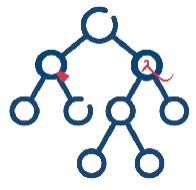
\includegraphics[height=1.0cm]{msca_logo.png}}%
    \end{center}

    \vspace{0.6cm}

    % Main title with Q logos on sides (with clickable links)
    \begin{center}
        \begin{minipage}{0.1\textwidth}
            \centering
            \href{https://quantlet.com}{
\includegraphics[height=1.1cm]{ql_logo.png}}
        \end{minipage}%
        \begin{minipage}{0.78\textwidth}
            \centering
            {\LARGE\bfseries\usebeamercolor[fg]{title}\inserttitle}

            \vspace{0.3cm}

            {\usebeamerfont{subtitle}\usebeamercolor[fg]{title}\insertsubtitle}
        \end{minipage}%
        \begin{minipage}{0.1\textwidth}
            \centering
            \href{https://quantinar.com}{
\includegraphics[height=1.1cm]{qr_logo.png}}
        \end{minipage}
    \end{center}

    \vspace{0.6cm}

    % Authors (left aligned)
    \hspace{0.5cm}{\usebeamerfont{author}\insertauthor}

    \vspace{0.3cm}

    % Institute/Affiliations (left aligned)
    \hspace{0.5cm}\begin{minipage}[t]{0.9\textwidth}
        \raggedright\small\insertinstitute
    \end{minipage}
}

%=============================================================================
% THEOREM ENVIRONMENTS
%=============================================================================
\theoremstyle{definition}
\setbeamertemplate{theorems}[numbered]
\ifdefined\atslang
\newtheorem{defn}{Definiție}
\newtheorem{thm}{Teoremă}
\newtheorem{prop}{Propoziție}
\newtheorem{rmk}{Observație}
\else
\newtheorem{defn}{Definition}
\newtheorem{thm}{Theorem}
\newtheorem{prop}{Proposition}
\newtheorem{rmk}{Remark}
\fi

%=============================================================================
% CENTRED MINIPAGE (no extra vertical space)
%=============================================================================
\newenvironment{cminipage}[1]{%
    \par\noindent\hfill\begin{minipage}{#1}\ignorespaces
}{%
    \end{minipage}\hfill\null\par
}

%=============================================================================
% CUSTOM COMMANDS
%=============================================================================
\newcommand{\E}{\mathbb{E}}
\newcommand{\Var}{\text{Var}}
\newcommand{\Cov}{\text{Cov}}
\newcommand{\Corr}{\text{Corr}}
\newcommand{\R}{\mathbb{R}}
\newcommand{\N}{\mathbb{N}}
\newcommand{\Z}{\mathbb{Z}}
\newcommand{\B}{\mathbf{B}}
\newcommand{\imark}{\textcolor{MainBlue}{\textbullet}}
\newcommand{\RMSE}{\text{RMSE}}
\newcommand{\MAE}{\text{MAE}}
\newcommand{\MAPE}{\text{MAPE}}

% Boldface vector/matrix commands (VAR, VECM, state space)
\newcommand{\bY}{\mathbf{Y}}
\newcommand{\bX}{\mathbf{X}}
\newcommand{\bA}{\mathbf{A}}
\newcommand{\bB}{\mathbf{B}}
\newcommand{\bepsilon}{\boldsymbol{\varepsilon}}
\newcommand{\bSigma}{\boldsymbol{\Sigma}}
\newcommand{\bPhi}{\boldsymbol{\Phi}}
\newcommand{\bGamma}{\boldsymbol{\Gamma}}
\newcommand{\bPi}{\boldsymbol{\Pi}}
\newcommand{\bc}{\mathbf{c}}
\newcommand{\balpha}{\boldsymbol{\alpha}}
\newcommand{\bbeta}{\boldsymbol{\beta}}
\newcommand{\bvarepsilon}{\boldsymbol{\varepsilon}}

% Seminar marks
\newcommand{\correct}{\textcolor{Forest}{\checkmark}}
\newcommand{\incorrect}{\textcolor{Crimson}{\texttimes}}
 se definește
%   \newcommand{\coursename}{Advanced Time Series Analysis and Forecasting}          (EN)
%   \newcommand{\coursename}{Analiza avansată a seriilor de timp și previziune}       (RO)  și  \def\atslang{ro}
% Fișierele .tex se află în EN/Courses, EN/Seminars, RO/Cursuri, RO/Seminarii (două niveluri sub rădăcină).
% Deck-urile sînt generate de latex/build_chapterN.py / build_seminarN.py (vezi latex/ats_build.py).

\documentclass[9pt, aspectratio=169, t]{beamer}
\providecommand{\coursename}{Advanced Time Series Analysis and Forecasting}

% Ensure content fits on slides
\setbeamersize{text margin left=8mm, text margin right=8mm}
% Smaller institute font (title page)
\setbeamerfont{institute}{size=\footnotesize}

%=============================================================================
% THEME AND STYLE CONFIGURATION
%=============================================================================
\usetheme{default}
% Using default theme for clean header/footer control

% Color Palette (matching Redispatch PDF)
\definecolor{MainBlue}{RGB}{26, 58, 110}
\definecolor{AccentBlue}{RGB}{26, 58, 110}
\definecolor{IDAred}{RGB}{205, 0, 0}
\definecolor{DarkGray}{RGB}{51, 51, 51}
\definecolor{MediumGray}{RGB}{128, 128, 128}
\definecolor{LightGray}{RGB}{248, 248, 248}
\definecolor{VeryLightGray}{RGB}{235, 235, 235}
\definecolor{KeynoteGray}{RGB}{218, 218, 218}
\definecolor{SectionGray}{RGB}{120, 120, 120}
\definecolor{FooterGray}{RGB}{100, 100, 100}
\definecolor{Crimson}{RGB}{220, 53, 69}
\definecolor{Forest}{RGB}{46, 125, 50}
\definecolor{Amber}{RGB}{181, 133, 63}
\definecolor{Orange}{RGB}{230, 126, 34}
\definecolor{Purple}{RGB}{142, 68, 173}

% Gradient background (exact Keynote 315° gradient: white to RGB 218,218,218)
\setbeamertemplate{background}{%
    \begin{tikzpicture}[remember picture, overlay]
        \shade[shading=axis, shading angle=315,
        top color=white, bottom color=KeynoteGray]
        (current page.south west) rectangle (current page.north east);
    \end{tikzpicture}%
}
% Fallback solid color for compatibility
\setbeamercolor{background canvas}{bg=}

\setbeamercolor{palette primary}{bg=MainBlue, fg=white}
\setbeamercolor{palette secondary}{bg=MainBlue!85, fg=white}
\setbeamercolor{palette tertiary}{bg=MainBlue!70, fg=white}
\setbeamercolor{structure}{fg=MainBlue}
\setbeamercolor{title}{fg=IDAred}
\setbeamercolor{frametitle}{fg=IDAred, bg=}
\setbeamercolor{block title}{bg=MainBlue, fg=white}
\setbeamercolor{block body}{bg=VeryLightGray, fg=DarkGray}
\setbeamercolor{block title alerted}{bg=Crimson, fg=white}
\setbeamercolor{block body alerted}{bg=Crimson!8, fg=DarkGray}
\setbeamercolor{block title example}{bg=Forest, fg=white}
\setbeamercolor{block body example}{bg=Forest!8, fg=DarkGray}
\setbeamercolor{item}{fg=MainBlue}

% Footer colors (override Madrid theme blue)
\setbeamercolor{author in head/foot}{fg=FooterGray, bg=}
\setbeamercolor{title in head/foot}{fg=FooterGray, bg=}
\setbeamercolor{date in head/foot}{fg=FooterGray, bg=}
\setbeamercolor{section in head/foot}{fg=FooterGray, bg=}
\setbeamercolor{subsection in head/foot}{fg=FooterGray, bg=}

% Bullet styles (apply everywhere including blocks)
\setbeamertemplate{itemize item}{\color{MainBlue}$\boxdot$}
\setbeamertemplate{itemize subitem}{\color{MainBlue}$\blacktriangleright$}
\setbeamertemplate{itemize subsubitem}{\color{MainBlue}\tiny$\bullet$}
\setbeamertemplate{itemize/enumerate body begin}{\normalsize}
\setbeamertemplate{itemize/enumerate subbody begin}{\normalsize}

% Item spacing - compact style
\setlength{\leftmargini}{10pt}       % Level 1: minimal indent
\setlength{\leftmarginii}{10pt}      % Level 2: minimal additional indent
% Compact list spacing (zero extra space before/after lists in blocks)
\makeatletter
\def\@listi{\leftmargin\leftmargini \topsep 0pt \parsep 0pt \itemsep 0pt}
\def\@listii{\leftmargin\leftmarginii \topsep 0pt \parsep 0pt \itemsep 0pt}
\makeatother

\setbeamertemplate{navigation symbols}{}

%=============================================================================
% CUSTOM HEADLINE
%=============================================================================
\setbeamertemplate{headline}{%
    \vskip10pt%
    \hbox to \paperwidth{%
        \hskip0.5cm%
        {\small\color{FooterGray}\renewcommand{\hyperlink}[2]{##2}\insertsectionhead}%
        \hfill%
        \textcolor{FooterGray}{\small\insertframenumber}%
        \hskip0.5cm%
    }%
    \vskip4pt%
    {\color{FooterGray}\hrule height 0.4pt}%
}

%=============================================================================
% CUSTOM FOOTER
%=============================================================================
\usepackage{fontawesome5}

\setbeamertemplate{footline}{%
    {\color{FooterGray}\hrule height 0.4pt}%
    \vskip4pt%
    \hbox to \paperwidth{%
        \hskip0.5cm%
        \textcolor{FooterGray}{\small\coursename}%
        \hfill%
        \raisebox{-0.1em}{%
            \begin{tikzpicture}[x=0.08em, y=0.08em, line width=0.4pt]
                \draw[FooterGray] (0,3) -- (1,4) -- (2,3.5) -- (3,5) -- (4,4) -- (5,6) -- (6,5.5) -- (7,4) -- (8,5) -- (9,7) -- (10,6) -- (11,5) -- (12,6.5) -- (13,8) -- (14,7) -- (15,6) -- (16,7.5) -- (17,9) -- (18,8) -- (19,7) -- (20,8.5) -- (21,10) -- (22,9) -- (23,8) -- (24,9.5);
            \end{tikzpicture}%
        }%
        \hskip0.5cm%
    }%
    \vskip6pt%
}

%=============================================================================
% PACKAGES
%=============================================================================
\usepackage[utf8]{inputenc}
\DeclareUnicodeCharacter{03B1}{\ensuremath{\alpha}}
\usepackage[T1]{fontenc}
\usepackage{amsmath, amssymb, amsthm}
\usepackage{mathtools}
\usepackage{bm}
\usepackage{tikz}
\usetikzlibrary{arrows.meta, positioning, shapes, calc, decorations.pathreplacing, shadings}
\usepackage{booktabs}
\usepackage{multirow}
\usepackage{array}
\usepackage{graphicx}
\usepackage{animate}
\usepackage{hyperref}
\usepackage{colortbl}
\usepackage{listings}
\lstset{language=Python, basicstyle=\ttfamily\scriptsize, keywordstyle=\color{MainBlue}\bfseries,
  commentstyle=\color{Forest}, stringstyle=\color{Crimson}, breaklines=true,
  frame=none, backgroundcolor=\color{VeryLightGray}, xleftmargin=2mm}
\hypersetup{colorlinks=true, linkcolor=MainBlue, urlcolor=MainBlue}
\graphicspath{{../../logos/}{../../charts/}{../../photos/}}
\usepackage{xcolor}
\hfuzz=2pt  % Suppress tiny overfull warnings (<2pt)
\vfuzz=2pt  % Suppress tiny vertical overfull warnings (<2pt)

%=============================================================================
% QUANTLET COMMANDS
%   \quantlet{<displayed name>}{<url>}       (generic)
%   \atsquantlet{Ch_05}{ATS_ch5_garch}       -> https://github.com/danpele/Advanced-Time-Series/tree/main/Quantlets/Ch_05/ATS_ch5_garch
%   \qlurl{<folder>} is defined per chapter by the generator (Quantlets/Ch_NN/<folder>)
%=============================================================================
\newcommand{\atsrepo}{https://github.com/danpele/Advanced-Time-Series}
\newcommand{\atsqlbase}{https://github.com/danpele/Advanced-Time-Series/tree/main/Quantlets}
\newcommand{\quantlet}[2]{%
    \hfill\href{#2}{%
        \raisebox{-0.15em}{
\includegraphics[height=0.7em]{ql_logo.png}}%
        \textcolor{MainBlue}{\tiny\ #1}%
    }%
}
\newcommand{\atsquantlet}[2]{\quantlet{\detokenize{#2}}{\atsqlbase/#1/#2}}

%=============================================================================
% NOTEBOOKS (Google Colab)
%   \colaburl{notebooks/EN/chapter5_seminar_notebook.ipynb} -> the Colab link of a file in the ATS repo
%   \nb: the chapter notebook (each seminar deck redefines it with \renewcommand)
%=============================================================================
\newcommand{\colaburl}[1]{https://colab.research.google.com/github/danpele/Advanced-Time-Series/blob/main/#1}
\newcommand{\nb}{https://colab.research.google.com/github/danpele/Advanced-Time-Series/tree/main/notebooks/EN}
\newcommand{\nbname}{notebooks/EN}

%=============================================================================
% SLIDE HELPERS (used by the generators; the same as in MFM)
%=============================================================================
% local font size for list bodies (the preamble forces \normalsize)
\newcommand{\itemsize}[1]{\setbeamertemplate{itemize/enumerate body begin}{#1}\setbeamertemplate{itemize/enumerate subbody begin}{#1}}
\newcommand{\intitle}[1]{{\hypersetup{urlcolor=white}#1}}   % white links inside coloured title bars
\newcommand{\imgcap}[1]{{\scriptsize #1}\\[0.5mm]}          % caption under a photo
\newcommand{\imgcredit}[2]{{\tiny\color{FooterGray}\href{#1}{#2}}}   % image credit: source URL, author/licence
\newcommand{\aiprompt}[1]{{\ttfamily\color{MainBlue}#1}}     % a prompt to an AI assistant

%=============================================================================
% SEMINARS: student version by default; the instructor wrapper *_solutions.tex sets \solutionstrue
%=============================================================================
\makeatletter\@ifundefined{ifsolutions}{\expandafter\newif\csname ifsolutions\endcsname}{}\makeatother
\newcommand{\solonly}[1]{\ifsolutions #1\fi}
\newcommand{\propsub}{\ifsolutions\else\framesubtitle{\ifdefined\atslang Rezolvarea se discută la seminar\else Solution discussed in class\fi}\fi}

%=============================================================================
% APPENDIX AND CHAPTER LINKS (latex/appendix_links.py writes the calls; it also re-declares these
% macros before \begin{document}, so the decks compile with or without this preamble block)
%=============================================================================
\providecommand{\atsapplink}[3]{\hypertarget{#2}{}\hyperlink{#1}{\beamergotobutton{#3}}}
\providecommand{\atsappback}[2]{\begin{tikzpicture}[remember picture,overlay]\node[anchor=south east] at ([xshift=-3mm,yshift=7mm]current page.south east){\hyperlink{#1}{\beamerreturnbutton{#2}}};\end{tikzpicture}}
\providecommand{\atschlink}[2]{\href{#1}{#2}}
\providecommand{\atschlinkt}[2]{\href{#1}{\usebeamercolor[fg]{frametitle}#2}}

%=============================================================================
% QUANTINAR COMMAND: link către un curs Quantinar (subiecte avansate)
%=============================================================================
\newcommand{\quantinar}[2]{%
    \href{#2}{%
        \raisebox{-0.15em}{
\includegraphics[height=0.8em]{qr_logo.png}}%
        \textcolor{MainBlue}{\scriptsize\ #1}%
    }%
}

%=============================================================================
% CUSTOM TITLE PAGE
%=============================================================================
\defbeamertemplate*{title page}{hybrid}[1][]
{
    \vspace{0.2cm}
    % Logos row - top header (with clickable links)
    \begin{center}
        \href{https://www.ase.ro}{
\includegraphics[height=1.0cm]{ase_logo.png}}\hspace{0.3cm}%
        \href{https://theida.net}{
\includegraphics[height=1.0cm]{ida_logo.png}}\hspace{0.3cm}%
        \href{https://blockchain-research-center.com}{
\includegraphics[height=1.0cm]{brc_logo.png}}\hspace{0.3cm}%
        \href{https://www.ai4efin.ase.ro}{
\includegraphics[height=1.0cm]{ai4efin_logo.png}}\hspace{0.3cm}%
        \href{https://ipe.ro/new}{
\includegraphics[height=1.0cm]{acad_logo.png}}\hspace{0.3cm}%
        \href{https://www.digital-finance-msca.com}{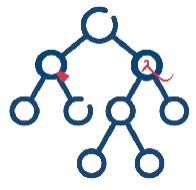
\includegraphics[height=1.0cm]{msca_logo.png}}%
    \end{center}

    \vspace{0.6cm}

    % Main title with Q logos on sides (with clickable links)
    \begin{center}
        \begin{minipage}{0.1\textwidth}
            \centering
            \href{https://quantlet.com}{
\includegraphics[height=1.1cm]{ql_logo.png}}
        \end{minipage}%
        \begin{minipage}{0.78\textwidth}
            \centering
            {\LARGE\bfseries\usebeamercolor[fg]{title}\inserttitle}

            \vspace{0.3cm}

            {\usebeamerfont{subtitle}\usebeamercolor[fg]{title}\insertsubtitle}
        \end{minipage}%
        \begin{minipage}{0.1\textwidth}
            \centering
            \href{https://quantinar.com}{
\includegraphics[height=1.1cm]{qr_logo.png}}
        \end{minipage}
    \end{center}

    \vspace{0.6cm}

    % Authors (left aligned)
    \hspace{0.5cm}{\usebeamerfont{author}\insertauthor}

    \vspace{0.3cm}

    % Institute/Affiliations (left aligned)
    \hspace{0.5cm}\begin{minipage}[t]{0.9\textwidth}
        \raggedright\small\insertinstitute
    \end{minipage}
}

%=============================================================================
% THEOREM ENVIRONMENTS
%=============================================================================
\theoremstyle{definition}
\setbeamertemplate{theorems}[numbered]
\ifdefined\atslang
\newtheorem{defn}{Definiție}
\newtheorem{thm}{Teoremă}
\newtheorem{prop}{Propoziție}
\newtheorem{rmk}{Observație}
\else
\newtheorem{defn}{Definition}
\newtheorem{thm}{Theorem}
\newtheorem{prop}{Proposition}
\newtheorem{rmk}{Remark}
\fi

%=============================================================================
% CENTRED MINIPAGE (no extra vertical space)
%=============================================================================
\newenvironment{cminipage}[1]{%
    \par\noindent\hfill\begin{minipage}{#1}\ignorespaces
}{%
    \end{minipage}\hfill\null\par
}

%=============================================================================
% CUSTOM COMMANDS
%=============================================================================
\newcommand{\E}{\mathbb{E}}
\newcommand{\Var}{\text{Var}}
\newcommand{\Cov}{\text{Cov}}
\newcommand{\Corr}{\text{Corr}}
\newcommand{\R}{\mathbb{R}}
\newcommand{\N}{\mathbb{N}}
\newcommand{\Z}{\mathbb{Z}}
\newcommand{\B}{\mathbf{B}}
\newcommand{\imark}{\textcolor{MainBlue}{\textbullet}}
\newcommand{\RMSE}{\text{RMSE}}
\newcommand{\MAE}{\text{MAE}}
\newcommand{\MAPE}{\text{MAPE}}

% Boldface vector/matrix commands (VAR, VECM, state space)
\newcommand{\bY}{\mathbf{Y}}
\newcommand{\bX}{\mathbf{X}}
\newcommand{\bA}{\mathbf{A}}
\newcommand{\bB}{\mathbf{B}}
\newcommand{\bepsilon}{\boldsymbol{\varepsilon}}
\newcommand{\bSigma}{\boldsymbol{\Sigma}}
\newcommand{\bPhi}{\boldsymbol{\Phi}}
\newcommand{\bGamma}{\boldsymbol{\Gamma}}
\newcommand{\bPi}{\boldsymbol{\Pi}}
\newcommand{\bc}{\mathbf{c}}
\newcommand{\balpha}{\boldsymbol{\alpha}}
\newcommand{\bbeta}{\boldsymbol{\beta}}
\newcommand{\bvarepsilon}{\boldsymbol{\varepsilon}}

% Seminar marks
\newcommand{\correct}{\textcolor{Forest}{\checkmark}}
\newcommand{\incorrect}{\textcolor{Crimson}{\texttimes}}
 se definește
%   \newcommand{\coursename}{Advanced Time Series Analysis and Forecasting}          (EN)
%   \newcommand{\coursename}{Analiza avansată a seriilor de timp și previziune}       (RO)  și  \def\atslang{ro}
% Fișierele .tex se află în EN/Courses, EN/Seminars, RO/Cursuri, RO/Seminarii (două niveluri sub rădăcină).
% Deck-urile sînt generate de latex/build_chapterN.py / build_seminarN.py (vezi latex/ats_build.py).

\documentclass[9pt, aspectratio=169, t]{beamer}
\providecommand{\coursename}{Advanced Time Series Analysis and Forecasting}

% Ensure content fits on slides
\setbeamersize{text margin left=8mm, text margin right=8mm}
% Smaller institute font (title page)
\setbeamerfont{institute}{size=\footnotesize}

%=============================================================================
% THEME AND STYLE CONFIGURATION
%=============================================================================
\usetheme{default}
% Using default theme for clean header/footer control

% Color Palette (matching Redispatch PDF)
\definecolor{MainBlue}{RGB}{26, 58, 110}
\definecolor{AccentBlue}{RGB}{26, 58, 110}
\definecolor{IDAred}{RGB}{205, 0, 0}
\definecolor{DarkGray}{RGB}{51, 51, 51}
\definecolor{MediumGray}{RGB}{128, 128, 128}
\definecolor{LightGray}{RGB}{248, 248, 248}
\definecolor{VeryLightGray}{RGB}{235, 235, 235}
\definecolor{KeynoteGray}{RGB}{218, 218, 218}
\definecolor{SectionGray}{RGB}{120, 120, 120}
\definecolor{FooterGray}{RGB}{100, 100, 100}
\definecolor{Crimson}{RGB}{220, 53, 69}
\definecolor{Forest}{RGB}{46, 125, 50}
\definecolor{Amber}{RGB}{181, 133, 63}
\definecolor{Orange}{RGB}{230, 126, 34}
\definecolor{Purple}{RGB}{142, 68, 173}

% Gradient background (exact Keynote 315° gradient: white to RGB 218,218,218)
\setbeamertemplate{background}{%
    \begin{tikzpicture}[remember picture, overlay]
        \shade[shading=axis, shading angle=315,
        top color=white, bottom color=KeynoteGray]
        (current page.south west) rectangle (current page.north east);
    \end{tikzpicture}%
}
% Fallback solid color for compatibility
\setbeamercolor{background canvas}{bg=}

\setbeamercolor{palette primary}{bg=MainBlue, fg=white}
\setbeamercolor{palette secondary}{bg=MainBlue!85, fg=white}
\setbeamercolor{palette tertiary}{bg=MainBlue!70, fg=white}
\setbeamercolor{structure}{fg=MainBlue}
\setbeamercolor{title}{fg=IDAred}
\setbeamercolor{frametitle}{fg=IDAred, bg=}
\setbeamercolor{block title}{bg=MainBlue, fg=white}
\setbeamercolor{block body}{bg=VeryLightGray, fg=DarkGray}
\setbeamercolor{block title alerted}{bg=Crimson, fg=white}
\setbeamercolor{block body alerted}{bg=Crimson!8, fg=DarkGray}
\setbeamercolor{block title example}{bg=Forest, fg=white}
\setbeamercolor{block body example}{bg=Forest!8, fg=DarkGray}
\setbeamercolor{item}{fg=MainBlue}

% Footer colors (override Madrid theme blue)
\setbeamercolor{author in head/foot}{fg=FooterGray, bg=}
\setbeamercolor{title in head/foot}{fg=FooterGray, bg=}
\setbeamercolor{date in head/foot}{fg=FooterGray, bg=}
\setbeamercolor{section in head/foot}{fg=FooterGray, bg=}
\setbeamercolor{subsection in head/foot}{fg=FooterGray, bg=}

% Bullet styles (apply everywhere including blocks)
\setbeamertemplate{itemize item}{\color{MainBlue}$\boxdot$}
\setbeamertemplate{itemize subitem}{\color{MainBlue}$\blacktriangleright$}
\setbeamertemplate{itemize subsubitem}{\color{MainBlue}\tiny$\bullet$}
\setbeamertemplate{itemize/enumerate body begin}{\normalsize}
\setbeamertemplate{itemize/enumerate subbody begin}{\normalsize}

% Item spacing - compact style
\setlength{\leftmargini}{10pt}       % Level 1: minimal indent
\setlength{\leftmarginii}{10pt}      % Level 2: minimal additional indent
% Compact list spacing (zero extra space before/after lists in blocks)
\makeatletter
\def\@listi{\leftmargin\leftmargini \topsep 0pt \parsep 0pt \itemsep 0pt}
\def\@listii{\leftmargin\leftmarginii \topsep 0pt \parsep 0pt \itemsep 0pt}
\makeatother

\setbeamertemplate{navigation symbols}{}

%=============================================================================
% CUSTOM HEADLINE
%=============================================================================
\setbeamertemplate{headline}{%
    \vskip10pt%
    \hbox to \paperwidth{%
        \hskip0.5cm%
        {\small\color{FooterGray}\renewcommand{\hyperlink}[2]{##2}\insertsectionhead}%
        \hfill%
        \textcolor{FooterGray}{\small\insertframenumber}%
        \hskip0.5cm%
    }%
    \vskip4pt%
    {\color{FooterGray}\hrule height 0.4pt}%
}

%=============================================================================
% CUSTOM FOOTER
%=============================================================================
\usepackage{fontawesome5}

\setbeamertemplate{footline}{%
    {\color{FooterGray}\hrule height 0.4pt}%
    \vskip4pt%
    \hbox to \paperwidth{%
        \hskip0.5cm%
        \textcolor{FooterGray}{\small\coursename}%
        \hfill%
        \raisebox{-0.1em}{%
            \begin{tikzpicture}[x=0.08em, y=0.08em, line width=0.4pt]
                \draw[FooterGray] (0,3) -- (1,4) -- (2,3.5) -- (3,5) -- (4,4) -- (5,6) -- (6,5.5) -- (7,4) -- (8,5) -- (9,7) -- (10,6) -- (11,5) -- (12,6.5) -- (13,8) -- (14,7) -- (15,6) -- (16,7.5) -- (17,9) -- (18,8) -- (19,7) -- (20,8.5) -- (21,10) -- (22,9) -- (23,8) -- (24,9.5);
            \end{tikzpicture}%
        }%
        \hskip0.5cm%
    }%
    \vskip6pt%
}

%=============================================================================
% PACKAGES
%=============================================================================
\usepackage[utf8]{inputenc}
\DeclareUnicodeCharacter{03B1}{\ensuremath{\alpha}}
\usepackage[T1]{fontenc}
\usepackage{amsmath, amssymb, amsthm}
\usepackage{mathtools}
\usepackage{bm}
\usepackage{tikz}
\usetikzlibrary{arrows.meta, positioning, shapes, calc, decorations.pathreplacing, shadings}
\usepackage{booktabs}
\usepackage{multirow}
\usepackage{array}
\usepackage{graphicx}
\usepackage{animate}
\usepackage{hyperref}
\usepackage{colortbl}
\usepackage{listings}
\lstset{language=Python, basicstyle=\ttfamily\scriptsize, keywordstyle=\color{MainBlue}\bfseries,
  commentstyle=\color{Forest}, stringstyle=\color{Crimson}, breaklines=true,
  frame=none, backgroundcolor=\color{VeryLightGray}, xleftmargin=2mm}
\hypersetup{colorlinks=true, linkcolor=MainBlue, urlcolor=MainBlue}
\graphicspath{{../../logos/}{../../charts/}{../../photos/}}
\usepackage{xcolor}
\hfuzz=2pt  % Suppress tiny overfull warnings (<2pt)
\vfuzz=2pt  % Suppress tiny vertical overfull warnings (<2pt)

%=============================================================================
% QUANTLET COMMANDS
%   \quantlet{<displayed name>}{<url>}       (generic)
%   \atsquantlet{Ch_05}{ATS_ch5_garch}       -> https://github.com/danpele/Advanced-Time-Series/tree/main/Quantlets/Ch_05/ATS_ch5_garch
%   \qlurl{<folder>} is defined per chapter by the generator (Quantlets/Ch_NN/<folder>)
%=============================================================================
\newcommand{\atsrepo}{https://github.com/danpele/Advanced-Time-Series}
\newcommand{\atsqlbase}{https://github.com/danpele/Advanced-Time-Series/tree/main/Quantlets}
\newcommand{\quantlet}[2]{%
    \hfill\href{#2}{%
        \raisebox{-0.15em}{
\includegraphics[height=0.7em]{ql_logo.png}}%
        \textcolor{MainBlue}{\tiny\ #1}%
    }%
}
\newcommand{\atsquantlet}[2]{\quantlet{\detokenize{#2}}{\atsqlbase/#1/#2}}

%=============================================================================
% NOTEBOOKS (Google Colab)
%   \colaburl{notebooks/EN/chapter5_seminar_notebook.ipynb} -> the Colab link of a file in the ATS repo
%   \nb: the chapter notebook (each seminar deck redefines it with \renewcommand)
%=============================================================================
\newcommand{\colaburl}[1]{https://colab.research.google.com/github/danpele/Advanced-Time-Series/blob/main/#1}
\newcommand{\nb}{https://colab.research.google.com/github/danpele/Advanced-Time-Series/tree/main/notebooks/EN}
\newcommand{\nbname}{notebooks/EN}

%=============================================================================
% SLIDE HELPERS (used by the generators; the same as in MFM)
%=============================================================================
% local font size for list bodies (the preamble forces \normalsize)
\newcommand{\itemsize}[1]{\setbeamertemplate{itemize/enumerate body begin}{#1}\setbeamertemplate{itemize/enumerate subbody begin}{#1}}
\newcommand{\intitle}[1]{{\hypersetup{urlcolor=white}#1}}   % white links inside coloured title bars
\newcommand{\imgcap}[1]{{\scriptsize #1}\\[0.5mm]}          % caption under a photo
\newcommand{\imgcredit}[2]{{\tiny\color{FooterGray}\href{#1}{#2}}}   % image credit: source URL, author/licence
\newcommand{\aiprompt}[1]{{\ttfamily\color{MainBlue}#1}}     % a prompt to an AI assistant

%=============================================================================
% SEMINARS: student version by default; the instructor wrapper *_solutions.tex sets \solutionstrue
%=============================================================================
\makeatletter\@ifundefined{ifsolutions}{\expandafter\newif\csname ifsolutions\endcsname}{}\makeatother
\newcommand{\solonly}[1]{\ifsolutions #1\fi}
\newcommand{\propsub}{\ifsolutions\else\framesubtitle{\ifdefined\atslang Rezolvarea se discută la seminar\else Solution discussed in class\fi}\fi}

%=============================================================================
% APPENDIX AND CHAPTER LINKS (latex/appendix_links.py writes the calls; it also re-declares these
% macros before \begin{document}, so the decks compile with or without this preamble block)
%=============================================================================
\providecommand{\atsapplink}[3]{\hypertarget{#2}{}\hyperlink{#1}{\beamergotobutton{#3}}}
\providecommand{\atsappback}[2]{\begin{tikzpicture}[remember picture,overlay]\node[anchor=south east] at ([xshift=-3mm,yshift=7mm]current page.south east){\hyperlink{#1}{\beamerreturnbutton{#2}}};\end{tikzpicture}}
\providecommand{\atschlink}[2]{\href{#1}{#2}}
\providecommand{\atschlinkt}[2]{\href{#1}{\usebeamercolor[fg]{frametitle}#2}}

%=============================================================================
% QUANTINAR COMMAND: link către un curs Quantinar (subiecte avansate)
%=============================================================================
\newcommand{\quantinar}[2]{%
    \href{#2}{%
        \raisebox{-0.15em}{
\includegraphics[height=0.8em]{qr_logo.png}}%
        \textcolor{MainBlue}{\scriptsize\ #1}%
    }%
}

%=============================================================================
% CUSTOM TITLE PAGE
%=============================================================================
\defbeamertemplate*{title page}{hybrid}[1][]
{
    \vspace{0.2cm}
    % Logos row - top header (with clickable links)
    \begin{center}
        \href{https://www.ase.ro}{
\includegraphics[height=1.0cm]{ase_logo.png}}\hspace{0.3cm}%
        \href{https://theida.net}{
\includegraphics[height=1.0cm]{ida_logo.png}}\hspace{0.3cm}%
        \href{https://blockchain-research-center.com}{
\includegraphics[height=1.0cm]{brc_logo.png}}\hspace{0.3cm}%
        \href{https://www.ai4efin.ase.ro}{
\includegraphics[height=1.0cm]{ai4efin_logo.png}}\hspace{0.3cm}%
        \href{https://ipe.ro/new}{
\includegraphics[height=1.0cm]{acad_logo.png}}\hspace{0.3cm}%
        \href{https://www.digital-finance-msca.com}{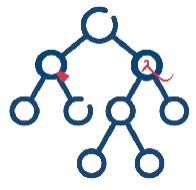
\includegraphics[height=1.0cm]{msca_logo.png}}%
    \end{center}

    \vspace{0.6cm}

    % Main title with Q logos on sides (with clickable links)
    \begin{center}
        \begin{minipage}{0.1\textwidth}
            \centering
            \href{https://quantlet.com}{
\includegraphics[height=1.1cm]{ql_logo.png}}
        \end{minipage}%
        \begin{minipage}{0.78\textwidth}
            \centering
            {\LARGE\bfseries\usebeamercolor[fg]{title}\inserttitle}

            \vspace{0.3cm}

            {\usebeamerfont{subtitle}\usebeamercolor[fg]{title}\insertsubtitle}
        \end{minipage}%
        \begin{minipage}{0.1\textwidth}
            \centering
            \href{https://quantinar.com}{
\includegraphics[height=1.1cm]{qr_logo.png}}
        \end{minipage}
    \end{center}

    \vspace{0.6cm}

    % Authors (left aligned)
    \hspace{0.5cm}{\usebeamerfont{author}\insertauthor}

    \vspace{0.3cm}

    % Institute/Affiliations (left aligned)
    \hspace{0.5cm}\begin{minipage}[t]{0.9\textwidth}
        \raggedright\small\insertinstitute
    \end{minipage}
}

%=============================================================================
% THEOREM ENVIRONMENTS
%=============================================================================
\theoremstyle{definition}
\setbeamertemplate{theorems}[numbered]
\ifdefined\atslang
\newtheorem{defn}{Definiție}
\newtheorem{thm}{Teoremă}
\newtheorem{prop}{Propoziție}
\newtheorem{rmk}{Observație}
\else
\newtheorem{defn}{Definition}
\newtheorem{thm}{Theorem}
\newtheorem{prop}{Proposition}
\newtheorem{rmk}{Remark}
\fi

%=============================================================================
% CENTRED MINIPAGE (no extra vertical space)
%=============================================================================
\newenvironment{cminipage}[1]{%
    \par\noindent\hfill\begin{minipage}{#1}\ignorespaces
}{%
    \end{minipage}\hfill\null\par
}

%=============================================================================
% CUSTOM COMMANDS
%=============================================================================
\newcommand{\E}{\mathbb{E}}
\newcommand{\Var}{\text{Var}}
\newcommand{\Cov}{\text{Cov}}
\newcommand{\Corr}{\text{Corr}}
\newcommand{\R}{\mathbb{R}}
\newcommand{\N}{\mathbb{N}}
\newcommand{\Z}{\mathbb{Z}}
\newcommand{\B}{\mathbf{B}}
\newcommand{\imark}{\textcolor{MainBlue}{\textbullet}}
\newcommand{\RMSE}{\text{RMSE}}
\newcommand{\MAE}{\text{MAE}}
\newcommand{\MAPE}{\text{MAPE}}

% Boldface vector/matrix commands (VAR, VECM, state space)
\newcommand{\bY}{\mathbf{Y}}
\newcommand{\bX}{\mathbf{X}}
\newcommand{\bA}{\mathbf{A}}
\newcommand{\bB}{\mathbf{B}}
\newcommand{\bepsilon}{\boldsymbol{\varepsilon}}
\newcommand{\bSigma}{\boldsymbol{\Sigma}}
\newcommand{\bPhi}{\boldsymbol{\Phi}}
\newcommand{\bGamma}{\boldsymbol{\Gamma}}
\newcommand{\bPi}{\boldsymbol{\Pi}}
\newcommand{\bc}{\mathbf{c}}
\newcommand{\balpha}{\boldsymbol{\alpha}}
\newcommand{\bbeta}{\boldsymbol{\beta}}
\newcommand{\bvarepsilon}{\boldsymbol{\varepsilon}}

% Seminar marks
\newcommand{\correct}{\textcolor{Forest}{\checkmark}}
\newcommand{\incorrect}{\textcolor{Crimson}{\texttimes}}


\newcommand{\qlurl}[1]{https://github.com/danpele/Advanced-Time-Series/tree/main/Quantlets/Ch_00/#1}

% Clickable citations (DOIs verified via Crossref)
\newcommand{\refHamilton}{\href{https://doi.org/10.2307/j.ctv14jx6sm}{Hamilton (1994)}}
\newcommand{\refKL}{\href{https://doi.org/10.1017/9781108164818}{Kilian și Lütkepohl (2017)}}
\newcommand{\refDK}{\href{https://doi.org/10.1093/acprof:oso/9780199641178.001.0001}{Durbin și Koopman (2012)}}
\newcommand{\refPetropoulos}{\href{https://doi.org/10.1016/j.ijforecast.2021.11.001}{Petropoulos et al.\ (2022)}}
\newcommand{\refHP}{\href{https://doi.org/10.1007/978-3-031-13584-2}{Huang și Petukhina (2022)}}
\newcommand{\refFPP}{\href{https://otexts.com/fpp3/}{Hyndman și Athanasopoulos (2021)}}
\newcommand{\refLutkepohl}{\href{https://doi.org/10.1007/978-3-540-27752-1}{Lütkepohl (2005)}}
\newcommand{\refSS}{\href{https://doi.org/10.1007/978-3-319-52452-8}{Shumway și Stoffer (2017)}}
\newcommand{\refBaltagi}{\href{https://doi.org/10.1007/978-3-030-53953-5}{Baltagi (2021)}}
\newcommand{\refAB}{\href{https://doi.org/10.1561/2200000101}{Angelopoulos și Bates (2023)}}
\newcommand{\refNW}{\href{https://doi.org/10.2307/1913610}{Newey și West (1987)}}
\newcommand{\refNWb}{\href{https://doi.org/10.2307/2297912}{Newey și West (1994)}}
\newcommand{\refAndrews}{\href{https://doi.org/10.2307/2938229}{Andrews (1991)}}
\newcommand{\refAM}{\href{https://doi.org/10.2307/2951574}{Andrews și Monahan (1992)}}
\newcommand{\refKunsch}{\href{https://doi.org/10.1214/aos/1176347265}{Künsch (1989)}}
\newcommand{\refLahiri}{\href{https://doi.org/10.1007/978-1-4757-3803-2}{Lahiri (2003)}}
\newcommand{\refPR}{\href{https://doi.org/10.1080/01621459.1994.10476870}{Politis și Romano (1994)}}
\newcommand{\refPW}{\href{https://doi.org/10.1081/ETC-120028836}{Politis și White (2004)}}
\newcommand{\refPPW}{\href{https://doi.org/10.1080/07474930802459016}{Patton, Politis și White (2009)}}
\newcommand{\refKV}{\href{https://doi.org/10.1017/S0266466605050565}{Kiefer și Vogelsang (2005)}}
\newcommand{\refKVB}{\href{https://doi.org/10.1111/1468-0262.00128}{Kiefer, Vogelsang și Bunzel (2000)}}
\newcommand{\refKVb}{\href{https://doi.org/10.1111/1468-0262.00366}{Kiefer și Vogelsang (2002)}}
\newcommand{\refLLSW}{\href{https://doi.org/10.1080/07350015.2018.1506926}{Lazarus et al.\ (2018)}}
\newcommand{\refLLS}{\href{https://doi.org/10.3982/ECTA15404}{Lazarus, Lewis și Stock (2021)}}
\newcommand{\refMuller}{\href{https://doi.org/10.1080/07350015.2014.931238}{Müller (2014)}}
\newcommand{\refSPJ}{\href{https://doi.org/10.1111/j.0012-9682.2008.00822.x}{Sun, Phillips și Jin (2008)}}
\newcommand{\refWhite}{\href{https://doi.org/10.1111/1468-0262.00152}{White (2000)}}
\newcommand{\refHansen}{\href{https://doi.org/10.1198/073500105000000063}{Hansen (2005)}}
\newcommand{\refRW}{\href{https://doi.org/10.1111/j.1468-0262.2005.00615.x}{Romano și Wolf (2005)}}
\newcommand{\refSTW}{\href{https://doi.org/10.1111/0022-1082.00163}{Sullivan, Timmermann și White (1999)}}
\newcommand{\refLM}{\href{https://doi.org/10.1093/rfs/3.3.431}{Lo și MacKinlay (1990)}}
\newcommand{\refHLZ}{\href{https://doi.org/10.1093/rfs/hhv059}{Harvey, Liu și Zhu (2016)}}
\newcommand{\refBH}{\href{https://doi.org/10.1111/j.2517-6161.1995.tb02031.x}{Benjamini și Hochberg (1995)}}
\newcommand{\refRosenblatt}{\href{https://doi.org/10.1073/pnas.42.1.43}{Rosenblatt (1956)}}
\newcommand{\refIbragimov}{\href{https://doi.org/10.1137/1107036}{Ibragimov (1962)}}
\newcommand{\refBrown}{\href{https://doi.org/10.1214/aoms/1177693494}{Brown (1971)}}
\newcommand{\refBillingsley}{\href{https://doi.org/10.1090/S0002-9939-1961-0126871-X}{Billingsley (1961)}}
\newcommand{\refPS}{\href{https://doi.org/10.1214/aos/1176348666}{Phillips și Solo (1992)}}
\newcommand{\refBradley}{\href{https://doi.org/10.1214/154957805100000104}{Bradley (2005)}}
\newcommand{\refCC}{\href{https://doi.org/10.1017/S0266466602181023}{Carrasco și Chen (2002)}}
\newcommand{\refMokkadem}{\href{https://doi.org/10.1016/0304-4149(88)90045-2}{Mokkadem (1988)}}
\newcommand{\refBirkhoff}{\href{https://doi.org/10.1073/pnas.17.2.656}{Birkhoff (1931)}}
\newcommand{\refWhiteH}{\href{https://doi.org/10.2307/1912934}{White (1980)}}
\newcommand{\refEfron}{\href{https://doi.org/10.1214/aos/1176344552}{Efron (1979)}}
\newcommand{\refSingh}{\href{https://doi.org/10.1214/aos/1176345636}{Singh (1981)}}
\newcommand{\refWu}{\href{https://doi.org/10.1214/aos/1176350142}{Wu (1986)}}
\newcommand{\refLiu}{\href{https://doi.org/10.1214/aos/1176351062}{Liu (1988)}}
\newcommand{\refMammen}{\href{https://doi.org/10.1214/aos/1176349025}{Mammen (1993)}}
\newcommand{\refShao}{\href{https://doi.org/10.1198/jasa.2009.tm08744}{Shao (2010)}}
\newcommand{\refBuhlmann}{\href{https://doi.org/10.2307/3318584}{Bühlmann (1997)}}
\newcommand{\refGK}{\href{https://doi.org/10.1016/j.jeconom.2003.10.030}{Gonçalves și Kilian (2004)}}
\newcommand{\refGN}{\href{https://doi.org/10.1016/0304-4076(74)90034-7}{Granger și Newbold (1974)}}
\newcommand{\refPhillips}{\href{https://doi.org/10.1016/0304-4076(86)90001-1}{Phillips (1986)}}
\newcommand{\refHH}{\href{https://doi.org/10.1086/260910}{Hansen și Hodrick (1980)}}
\newcommand{\refEH}{\href{https://doi.org/10.1111/j.1540-6261.1991.tb02674.x}{Estrella și Hardouvelis (1991)}}
\newcommand{\refVilhuber}{\href{https://doi.org/10.1162/99608f92.4f6b9e67}{Vilhuber (2020)}}
\newcommand{\refCM}{\href{https://doi.org/10.1257/jel.20171350}{Christensen și Miguel (2018)}}
\newcommand{\refCS}{\href{https://doi.org/10.1016/S0304-4076(01)00072-0}{Croushore și Stark (2001)}}

\title[Analiza avansată a seriilor de timp și previziune]{Analiza avansată a seriilor de timp și previziune}
\subtitle{Capitolul 0: Recapitulare și inferență pentru date dependente}
\author[D.T. Pele]{Daniel Traian PELE}
\institute{Academia de Studii Economice din București\\
IDA Institute Digital Assets\\
Blockchain Research Center\\
AI4EFin Artificial Intelligence for Energy Finance\\
Academia Română, Institutul de Prognoză Economică\\
MSCA Digital Finance}
\date{}

%=============================================================================
\providecommand{\atsapplink}[3]{\hypertarget{#2}{}\hyperlink{#1}{\beamergotobutton{#3}}}  % APPLINKS-MACROS
\providecommand{\atsappback}[2]{\begin{tikzpicture}[remember picture,overlay]\node[anchor=south east] at ([xshift=-3mm,yshift=7mm]current page.south east){\hyperlink{#1}{\beamerreturnbutton{#2}}};\end{tikzpicture}}  % APPLINKS-MACROS
\providecommand{\atschlink}[2]{\href{#1}{#2}}  % APPLINKS-MACROS
\providecommand{\atschlinkt}[2]{\href{#1}{\usebeamercolor[fg]{frametitle}#2}}  % APPLINKS-MACROS
\begin{document}
%=============================================================================

{
\setbeamertemplate{headline}{}
\setbeamertemplate{footline}{}
\begin{frame}[noframenumbering]
    \titlepage
\end{frame}
}
% BEGIN-ACRONYMS (generat de latex/acronyms.py; nu editati manual)
\begin{frame}{Acronime folosite în acest material (1/2)}
\setbeamertemplate{itemize/enumerate body begin}{\tiny}
\begin{columns}[T]
\begin{column}{0.49\textwidth}
\begin{itemize}\setlength{\itemsep}{0pt}
    \item \textbf{ACF}: Autocorrelation Function (funcția de autocorelație)
    \item \textbf{AI}: Artificial Intelligence (inteligență artificială)
    \item \textbf{ALFRED}: ArchivaL Federal Reserve Economic Data (arhiva vintage-urilor FRED (Fed St. Louis))
    \item \textbf{AR}: AutoRegressive (model) — model autoregresiv
    \item \textbf{ARDL}: AutoRegressive Distributed Lag (model) — model autoregresiv cu decalaje distribuite
    \item \textbf{ARIMA}: AutoRegressive Integrated Moving Average (model) — model autoregresiv integrat cu medie mobilă
    \item \textbf{ARMA}: AutoRegressive Moving Average (model) — model autoregresiv cu medie mobilă
    \item \textbf{ASDS}: Statistică aplicată și data science
    \item \textbf{ASE}: Academia de Studii Economice din București
    \item \textbf{ATS}: Advanced Time Series Analysis and Forecasting (Analiza avansată a seriilor de timp și previziune, cursul de master)
    \item \textbf{BCE}: Banca Centrală Europeană
    \item \textbf{BET}: Bucharest Exchange Trading (index) — indicele de referință al Bursei de Valori București
    \item \textbf{BNR}: Banca Națională a României
\end{itemize}
\end{column}
\begin{column}{0.49\textwidth}
\begin{itemize}\setlength{\itemsep}{0pt}
    \item \textbf{BVAR}: Bayesian Vector AutoRegression (model vector autoregresiv bayesian)
    \item \textbf{CBB}: Circular Block Bootstrap (bootstrap circular pe blocuri)
    \item \textbf{DGP}: Data-Generating Process (procesul generator al datelor)
    \item \textbf{ECTS}: European Credit Transfer and Accumulation System (sistemul european de credite transferabile)
    \item \textbf{EOD}: End Of Day (daily closing data) — date de sfîrșit de zi, adică prețuri de închidere
    \item \textbf{EODHD}: EOD Historical Data (market-data provider) — furnizor de date de piață
    \item \textbf{ES}: Expected Shortfall (pierderea așteptată în coadă)
    \item \textbf{EWC}: Equal-Weighted Cosine (estimator) — estimatorul cu cosinusuri ponderate egal
    \item \textbf{FDR}: False Discovery Rate (rata descoperirilor false)
    \item \textbf{FM-OLS}: Fully Modified Ordinary Least Squares (metoda celor mai mici pătrate complet modificată)
    \item \textbf{FRED}: Federal Reserve Economic Data (baza de date economice a Rezervei Federale din St. Louis)
    \item \textbf{FWER}: Family-Wise Error Rate (probabilitatea de cel puțin o eroare de tip I în familia de teste)
    \item \textbf{GARCH}: Generalised AutoRegressive Conditional Heteroskedasticity (heteroscedasticitate condiționată autoregresivă generalizată)
\end{itemize}
\end{column}
\end{columns}
\end{frame}
\begin{frame}{Acronime folosite în acest material (2/2)}
\setbeamertemplate{itemize/enumerate body begin}{\tiny}
\begin{columns}[T]
\begin{column}{0.49\textwidth}
\begin{itemize}\setlength{\itemsep}{0pt}
    \item \textbf{HAC}: Heteroskedasticity and Autocorrelation Consistent (standard errors) — erori standard robuste la heteroscedasticitate și autocorelație
    \item \textbf{HAR}: Heterogeneous AutoRegressive (model) — model autoregresiv heterogen
    \item \textbf{IAPC}: Indicele armonizat al prețurilor de consum
    \item \textbf{INS}: Institutul Național de Statistică
    \item \textbf{IPC}: Indicele prețurilor de consum
    \item \textbf{KPSS}: Kwiatkowski–Phillips–Schmidt–Shin (test) — testul de staționaritate Kwiatkowski–Phillips–Schmidt–Shin
    \item \textbf{LGN}: Legea numerelor mari
    \item \textbf{LLSW}: Lazarus, Lewis, Stock and Watson (2018) — Lazarus, Lewis, Stock și Watson (2018)
    \item \textbf{MA}: Moving Average (medie mobilă)
    \item \textbf{MBB}: Moving-Block Bootstrap (bootstrap pe blocuri mobile)
    \item \textbf{MCMMP}: Metoda celor mai mici pătrate
    \item \textbf{MDS}: Martingale Difference Sequence (secvență de diferențe de martingală)
    \item \textbf{MFM}: Modelling Financial Markets (Modelarea piețelor financiare, cursul de master)
\end{itemize}
\end{column}
\begin{column}{0.49\textwidth}
\begin{itemize}\setlength{\itemsep}{0pt}
    \item \textbf{NW}: Newey–West (standard errors) — erori standard Newey–West
    \item \textbf{NW-A}: Newey–West with the Andrews (1991) bandwidth (Newey–West cu lățimea de bandă Andrews (1991))
    \item \textbf{PIB}: Produsul intern brut
    \item \textbf{QR}: Quick Response (code) — cod de răspuns rapid
    \item \textbf{QS}: Quadratic Spectral (kernel) — nucleul spectral pătratic
    \item \textbf{SARIMA}: Seasonal ARIMA (model) — model ARIMA sezonier
    \item \textbf{SPA}: Superior Predictive Ability (test) — testul abilității predictive superioare
    \item \textbf{SUA}: Statele Unite ale Americii
    \item \textbf{TLC}: Teorema Limită Centrală
    \item \textbf{TSA}: Time Series Analysis (Serii de timp, cursul de licență)
    \item \textbf{UE}: Uniunea Europeană
    \item \textbf{VAR}: Vector AutoRegression (model vector autoregresiv)
    \item \textbf{VECM}: Vector Error Correction Model (model vectorial cu corecția erorii)
\end{itemize}
\end{column}
\end{columns}
\end{frame}
% END-ACRONYMS

%=============================================================================
\section{Organizarea cursului}
%=============================================================================

\begin{frame}{Cursul pe scurt}
\itemsize{\footnotesize}
\begin{columns}[T]
\begin{column}{0.56\textwidth}
\begin{itemize}
    \item \textbf{Program}
    \begin{itemize}
        \item Programul de master Statistică aplicată și data science (ASDS), anul I, semestrul 2
        \item Facultatea de Cibernetică, Statistică și Informatică Economică, ASE București
        \item 7 credite ECTS; 2 ore de curs și 2 ore de seminar pe săptămînă; anul universitar 2026/2027
    \end{itemize}
    \item \textbf{Titular}
    \begin{itemize}
        \item Prof.\ Daniel Traian Pele, \href{mailto:danpele@ase.ro}{danpele@ase.ro}
    \end{itemize}
    \item \textbf{Site-ul cursului}
    \begin{itemize}
        \item \href{https://danpele.github.io/Advanced-Time-Series/}{danpele.github.io/Advanced-Time-Series}
        \item slide-uri, seminarii, notebook-uri, Quantlets și quiz-urile notate
    \end{itemize}
\end{itemize}
\end{column}
\begin{column}{0.40\textwidth}
\centering
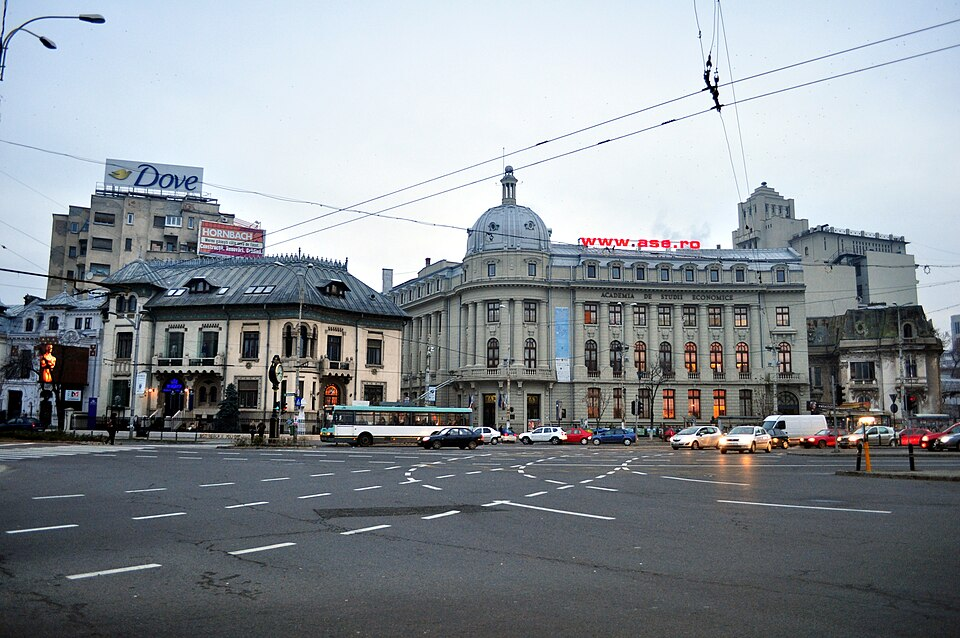
\includegraphics[height=0.46\textheight]{ch0_ase_2014.jpg}\\[1mm]
\imgcap{Academia de Studii Economice din București (ASE)}
\imgcredit{https://commons.wikimedia.org/wiki/File:Bucharest_-_Academie_de_Studii_Economice_01.jpg}{Foto: Joe Mabel (2014); CC BY 3.0; Wikimedia Commons}
\end{column}
\end{columns}
\end{frame}

\begin{frame}{Locul cursului în program}
\itemsize{\footnotesize}
\begin{itemize}
    \item \textbf{Înainte}: \href{https://danpele.github.io/Time-Series-Analysis/}{Serii de timp} (TSA, licență), capitolele 0--10 din TSA
    \begin{itemize}
        \item ARMA, ARIMA și rădăcini unitare, SARIMA, GARCH, VAR și cauzalitate Granger, cointegrare și VECM, memorie lungă, machine learning, modele în spațiul stărilor
        \item sînt considerate cunoscute: cursul pornește de la ele și nu le reia
    \end{itemize}
    \item \textbf{Acest curs}: ATS, master, anul I, semestrul 2
    \begin{itemize}
        \item metodologia prognozei, a identificării și a inferenței pentru date dependente
        \item serii macroeconomice (România și Uniunea Europeană), energetice, climatice și financiare
    \end{itemize}
    \item \textbf{După}: \href{https://danpele.github.io/MFM/}{Modelarea piețelor financiare} (MFM, master, anul II, semestrul 1)
    \begin{itemize}
        \item aceleași metode aplicate riscului de piață, portofoliilor, microstructurii și activelor digitale
    \end{itemize}
\end{itemize}
\end{frame}

\begin{frame}{Evaluare}
\itemsize{\small}
\begin{itemize}
    \item \textbf{Proiect de echipă și susținere orală individuală: 70\%}
    \begin{itemize}
        \item propunerea și preînregistrarea (echipă): 5\%
        \item replicarea și extensia: repository, raport, AI\_USE.md și AI\_ERRORS.md (echipă): 15\%
        \item susținerea orală individuală: 50\%
    \end{itemize}
    \item \textbf{Quiz-uri pe capitole: 20\%}
    \begin{itemize}
        \item online, pe site-ul cursului, cu contul Google ASE
    \end{itemize}
    \item \textbf{Prezență: 10\%}
    \begin{itemize}
        \item înregistrată prin formularul de prezență sau prin codul QR
    \end{itemize}
    \item Cursul nu are examen scris
\end{itemize}
\end{frame}

\begin{frame}{Manuale}
\itemsize{\small}
\begin{itemize}
    \item \textbf{Referințe principale}
    \begin{itemize}
        \item \refHamilton: teoria seriilor de timp liniare, rădăcini unitare și modele VAR
        \item \refKL: analiza VAR structurală și identificarea
        \item \refDK: metode în spațiul stărilor
        \item \refPetropoulos: teoria și practica prognozei, cu acces liber
    \end{itemize}
    \item \textbf{Legătura cu cursul de licență}
    \begin{itemize}
        \item \refHP; \refFPP
    \end{itemize}
    \item \textbf{Lucrări de specialitate}
    \begin{itemize}
        \item \refLutkepohl; \refSS; \refBaltagi; \refAB; pentru acest capitol și \refLahiri
        \item fiecare capitol adaugă lucrările de referință folosite ca studii de caz
    \end{itemize}
\end{itemize}
\end{frame}

\begin{frame}{Harta cursului (1/2)}
\begin{center}
\footnotesize
\begin{tabular}{rl}
\toprule
\textbf{Cap.} & \textbf{Tema} \\
\midrule
0 & Recapitulare și inferență pentru date dependente \\
1 & Evaluarea prognozelor, reguli de scor și combinarea prognozelor \\
2 & Rupturi structurale și modele neliniare \\
3 & Modele VAR structurale și proiecții locale \\
4 & Cointegrare: VECM, ARDL și date panel \\
5 & Modele VAR bayesiene, modele factoriale și nowcasting \\
6 & Modele în spațiul stărilor și filtrare bayesiană \\
7 & Modele cu schimbare de regim \\
8 & Modelarea avansată a volatilității: măsuri realizate, HAR și GARCH multivariat \\
\bottomrule
\end{tabular}
\end{center}
\end{frame}

\begin{frame}{Harta cursului (2/2)}
\begin{center}
\footnotesize
\begin{tabular}{rl}
\toprule
\textbf{Cap.} & \textbf{Tema} \\
\midrule
9 & VaR, ES și backtesting: elicitabilitate, funcții de scor și riscul de model \\
10 & Memorie lungă și rough volatility \\
11 & Analiză spectrală și analiză wavelet \\
12 & Machine learning și deep learning pentru serii de timp \\
13 & Foundation models și predicție conformală \\
14 & Inferență cauzală pentru serii de timp \\
15 & Recapitulare și susținerea proiectelor \\
16 & Rădăcini explozive și bule speculative (studiu individual) \\
\bottomrule
\end{tabular}
\end{center}
\end{frame}

\begin{frame}{Cursuri și seminarii}
\itemsize{\footnotesize}
\begin{itemize}
    \item \textbf{Cursuri}
    \begin{itemize}
        \item cîte un capitol pe săptămînă, construit în jurul unor lucrări de referință replicate pe datele noastre
        \item fiecare curs se încheie cu o secțiune despre AI în descoperirea științifică
    \end{itemize}
    \item \textbf{Seminarii}: fiecare seminar are loc \emph{înaintea} cursului și începe cu noțiunile necesare
    \begin{itemize}
        \item Partea A: derivări; Partea B: estimare și inferență pe date, fiecare exercițiu încheindu-se cu o întrebare de interpretare; Partea C: probleme deschise, care pot deveni idei de proiect
        \item exerciții [Rezolvat], cu soluții complete, și exerciții [Propus], discutate la seminar
        \item fiecare seminar include analiza critică a unui răspuns dat de un instrument AI
    \end{itemize}
    \item Seminarul are rol de exercițiu și nu se notează; rezolvările cerințelor [Propus] se discută la seminar
\end{itemize}
\end{frame}

\begin{frame}{Proiectul de echipă}
\itemsize{\footnotesize}
\begin{itemize}
    \item \textbf{Echipe de cel mult 3 studenți}
    \begin{itemize}
        \item replicarea unei lucrări de referință a cursului sau a unei alte lucrări aprobate de titular
        \item extinderea ei cu metodele cursului, de preferință pe date din România sau din Uniunea Europeană
    \end{itemize}
    \item \textbf{Etape}
    \begin{itemize}
        \item Etapa 1: întrebarea de cercetare, datele și un plan de evaluare fixat înaintea oricărei estimări (preînregistrare)
        \item Etapa 2: replicarea, extensia și un repository GitHub care reproduce fiecare rezultat (Colab)
        \item Etapa 3: prezentarea și susținerea orală individuală
    \end{itemize}
    \item Inferența validă pentru date dependente (acest capitol) face parte din fiecare proiect
    \item Proiectul poate fi redactat și susținut în limba română sau în limba engleză
\end{itemize}
\end{frame}

\begin{frame}{Politica privind AI}
\itemsize{\small}
\begin{itemize}
    \item \textbf{Permis și declarat}
    \begin{itemize}
        \item AI\_USE.md: instrumentul, scopul, prompturile, ce s-a păstrat și ce s-a modificat
        \item AI\_ERRORS.md: cel puțin trei erori ale instrumentelor AI depistate de echipă și modul în care a fost depistată fiecare
        \item folosirea nedeclarată este considerată plagiat
    \end{itemize}
    \item \textbf{Verificat}
    \begin{itemize}
        \item fiecare referință după DOI, fiecare rezultat numeric pe date și pe cod
    \end{itemize}
    \item \textbf{Susținerea orală fără AI}
    \begin{itemize}
        \item fiecare membru explică metodele, codul și rezultatele
    \end{itemize}
\end{itemize}
\end{frame}

\begin{frame}{Materiale și instrumente}
\itemsize{\small}
\begin{itemize}
    \item \textbf{Pentru fiecare capitol}
    \begin{itemize}
        \item slide-urile cursului și ale seminarului, în engleză și în română
        \item notebook-uri de curs și de seminar în engleză, rulabile în Google Colab
        \item un Quantlet cu codul fiecărui grafic și un quiz
    \end{itemize}
    \item \textbf{Date}
    \begin{itemize}
        \item date zilnice de piață de la EODHD (EOD Historical Data), salvate în repository-ul cursului
        \item date macroeconomice publice: INS, BNR, Eurostat, BCE și FRED
    \end{itemize}
    \item \textbf{Programe}
    \begin{itemize}
        \item Python: statsmodels, arch, linearmodels, scikit-learn, PyTorch
    \end{itemize}
\end{itemize}
\end{frame}


%=============================================================================
\section{Capitolul 0: planul}
%=============================================================================

\begin{frame}{Rezultatele învățării}
\itemsize{\small}
\begin{itemize}
    \item Să enunțați teoremele limită din spatele oricărei erori standard folosite pentru serii de timp: LGN ergodică, TLC pentru diferențe de martingală și pentru procese mixing
    \item Să derivați varianța de termen lung și consecințele ei pentru testele $t$ și intervalele de încredere
    \item Să alegeți și să argumentați un estimator HAC: nucleul, lățimea de bandă, valorile critice (standard sau fixed-$b$)
    \item Să folosiți bootstrap pe blocuri (mobile, circulare, staționar) și să știți cînd wild bootstrap nu este suficient
    \item Să măsurați distorsiunile de mărime prin Monte Carlo și să controlați data snooping
    \item Să construiți un pachet de replicare care reproduce fiecare rezultat al unui proiect
\end{itemize}
\end{frame}

\begin{frame}{Datele folosite în acest capitol}
\itemsize{\footnotesize}
\begin{center}
\scriptsize
\begin{tabular}{p{3.3cm}p{5.4cm}p{2.6cm}p{2.0cm}}
\toprule
\textbf{Seria} & \textbf{Definiție} & \textbf{Perioada} & \textbf{Sursa} \\
\midrule
Inflația în România & IAPC, rata anuală de variație, \%, lunar & ianuarie 2006 -- august 2026 & Eurostat \\
PIB-ul real al României & volume înlănțuite, ajustate sezonier; creștere t/t, \% & 2000Q1 -- 2026Q2 & Eurostat \\
EUR/RON & cursul de referință BNR; variația logaritmică zilnică, \% & 5 iulie 2005 -- 18 septembrie 2026 & BNR \\
S\&P 500, BET & randamente logaritmice zilnice și pătratele lor, \% & 2000 -- 18 septembrie 2026 & EODHD \\
Macro SUA & PIB real; randamentele titlurilor de stat la 10 ani și la 3 luni & 1962 -- 2026 & FRED \\
\bottomrule
\end{tabular}
\end{center}
\begin{itemize}
    \item Seriile zilnice pe calendarele lor de tranzacționare; seriile Eurostat și FRED citite online la data generării
    \item IAPC: indicele armonizat al prețurilor de consum; ținta BNR este definită pe IPC național, apropiat de IAPC
\end{itemize}
\end{frame}

\begin{frame}{Proveniența datelor}
\itemsize{\footnotesize}
\begin{columns}[T]
\begin{column}{0.48\textwidth}
\centering

\includegraphics[height=0.40\textheight]{ch0_bnr_palace_2015.jpg}\\[1mm]
\imgcap{Banca Națională a României (BNR), București: cursurile de referință și ținta de inflație}
\imgcredit{https://commons.wikimedia.org/wiki/File:Bucharest_-_BNR_Palace_(19644434340).jpg}{Foto: Ștefan Jurcă (2015); CC BY 2.0; Wikimedia Commons}
\end{column}
\begin{column}{0.48\textwidth}
\centering

\includegraphics[height=0.40\textheight]{ch0_eccles_2011.jpg}\\[1mm]
\imgcap{Clădirea Eccles, Washington: Consiliul Rezervei Federale; FRED este administrat de Fed St.\ Louis}
\imgcredit{https://commons.wikimedia.org/wiki/File:Eccles_Building_(26088200676).jpg}{Foto: Federal Reserve (2011); domeniu public; Wikimedia Commons}
\end{column}
\end{columns}\begin{itemize}
    \item O bancă centrală publică seriile pe care le testăm: ținta de inflație a BNR este 2,5\% $\pm$ 1 pp din 2013 (mini-studiul de caz de la final)
\end{itemize}
\end{frame}

\begin{frame}{Notații}
\itemsize{\small}
\begin{itemize}
    \item $\{x_t\}$ o serie (slab) staționară cu media $\mu$ și autocovarianțele $\gamma_j = \Cov(x_t, x_{t-j})$; $\rho_j = \gamma_j/\gamma_0$
    \item Media de selecție $\bar{x} = T^{-1}\sum_{t=1}^{T} x_t$; autocovarianța de selecție $\hat\gamma_j = T^{-1}\sum_{t=j+1}^{T}(x_t - \bar x)(x_{t-j} - \bar x)$
    \item Varianța de termen lung $\Omega = \sum_{j=-\infty}^{\infty}\gamma_j = 2\pi f(0)$, unde $f$ este densitatea spectrală
    \item Nucleul $k(\cdot)$, lățimea de bandă $S$ (decalajele Newey--West $L = S - 1$ pentru Bartlett), $b = S/T$
    \item Mărimea testului: probabilitatea de a respinge o ipoteză $H_0$ adevărată; nivelul nominal este $5\%$, dacă nu se precizează altfel
    \item HAC: consistent la heteroscedasticitate și autocorelație; HAR: robust la heteroscedasticitate și autocorelație (testul construit pe un estimator HAC)
\end{itemize}
\end{frame}


%=============================================================================
\section{Harta recapitulării din TSA}
%=============================================================================

\begin{frame}{Cunoștințe din TSA (licență)}
\itemsize{\footnotesize}
\begin{center}
\scriptsize
\begin{tabular}{p{3.2cm}p{2.6cm}p{7.2cm}}
\toprule
\textbf{Tema} & \textbf{TSA} & \textbf{Folosit în ATS pentru} \\
\midrule
Staționaritate, ACF, Wold & \atschlink{https://danpele.github.io/Time-Series-Analysis/RO/Cursuri/capitol1_procese_stochastice_stationaritate.pdf}{TSA, Capitolul 1} & varianța de termen lung, HAC, bootstrap (acest capitol) \\
ARMA & \atschlink{https://danpele.github.io/Time-Series-Analysis/RO/Cursuri/capitol2_modele_arma.pdf}{TSA, Capitolul 2} & modele de referință, planuri Monte Carlo, sieve bootstrap \\
Rădăcini unitare, ARIMA & \atschlink{https://danpele.github.io/Time-Series-Analysis/RO/Cursuri/capitol3_radacini_unitare_modele_arima.pdf}{TSA, Capitolul 3} & asimptotică nestandard, regresie falsă, \atschlink{https://danpele.github.io/Advanced-Time-Series/RO/Cursuri/capitol2_rupturi_structurale_modele_neliniare.pdf}{capitolele 2}, \atschlink{https://danpele.github.io/Advanced-Time-Series/RO/Cursuri/capitol4_cointegrare_vecm_ardl_panel.pdf}{4}, \atschlink{https://danpele.github.io/Advanced-Time-Series/RO/Cursuri/capitol16_radacini_explozive_bule_speculative.pdf}{16} \\
GARCH & \atschlink{https://danpele.github.io/Time-Series-Analysis/RO/Cursuri/capitol5_volatilitate_conditionata_garch.pdf}{TSA, Capitolul 5} & diferențe de martingală, \atschlink{https://danpele.github.io/Advanced-Time-Series/RO/Cursuri/capitol8_volatilitate_avansata.pdf}{capitolele 8}--\atschlink{https://danpele.github.io/Advanced-Time-Series/RO/Cursuri/capitol9_var_es_backtesting.pdf}{9} \\
VAR, Granger & \atschlink{https://danpele.github.io/Time-Series-Analysis/RO/Cursuri/capitol6_modele_var_cauzalitate_granger.pdf}{TSA, Capitolul 6} & VAR structural, proiecții locale, BVAR (\atschlink{https://danpele.github.io/Advanced-Time-Series/RO/Cursuri/capitol3_modele_var_structurale_proiectii_locale.pdf}{capitolele 3}, \atschlink{https://danpele.github.io/Advanced-Time-Series/RO/Cursuri/capitol5_bvar_modele_factoriale_nowcasting.pdf}{5}) \\
Cointegrare, VECM & \atschlink{https://danpele.github.io/Time-Series-Analysis/RO/Cursuri/capitol7_cointegrare_vecm.pdf}{TSA, Capitolul 7} & ARDL, cointegrare panel (\atschlink{https://danpele.github.io/Advanced-Time-Series/RO/Cursuri/capitol4_cointegrare_vecm_ardl_panel.pdf}{Capitolul 4}) \\
Memorie lungă & \atschlink{https://danpele.github.io/Time-Series-Analysis/RO/Cursuri/capitol8_memorie_lunga_arfima.pdf}{TSA, Capitolul 8} & local Whittle, rough volatility (\atschlink{https://danpele.github.io/Advanced-Time-Series/RO/Cursuri/capitol10_memorie_lunga_rough_volatility.pdf}{Capitolul 10}) \\
Spațiul stărilor, Markov switching & \atschlink{https://danpele.github.io/Time-Series-Analysis/RO/Cursuri/capitol10_spatiul_starilor_kalman_markov_switching.pdf}{TSA, Capitolul 10} & filtrare și regimuri (\atschlink{https://danpele.github.io/Advanced-Time-Series/RO/Cursuri/capitol6_modele_spatiul_starilor_filtrare_bayesiana.pdf}{capitolele 6}, \atschlink{https://danpele.github.io/Advanced-Time-Series/RO/Cursuri/capitol7_modele_schimbare_regim.pdf}{7}) \\
\bottomrule
\end{tabular}
\end{center}
\begin{itemize}
    \item Slide-urile cursului de licență: de la \atschlink{https://danpele.github.io/Time-Series-Analysis/RO/Cursuri/capitol1_procese_stochastice_stationaritate.pdf}{TSA, Capitolul 1} la \atschlink{https://danpele.github.io/Time-Series-Analysis/RO/Cursuri/capitol10_spatiul_starilor_kalman_markov_switching.pdf}{TSA, Capitolul 10}; fiecare capitol ATS trimite la capitolul TSA pe care îl continuă
\end{itemize}
\end{frame}

\begin{frame}{Staționaritatea și reprezentarea Wold}
\itemsize{\small}
\begin{itemize}
    \item \atschlink{https://danpele.github.io/Time-Series-Analysis/RO/Cursuri/capitol1_procese_stochastice_stationaritate.pdf}{TSA, Capitolul 1}. Staționaritate slabă: medie constantă și $\gamma_j$ care depinde doar de $j$; strictă: toate distribuțiile finit-dimensionale sînt invariante la translație
    \begin{itemize}
        \item Niciuna nu o implică pe cealaltă fără condiții de momente (Cauchy i.i.d.\ este strict, dar nu slab staționar)
    \end{itemize}
    \item Wold: orice serie slab staționară, pur nedeterministă, este $x_t - \mu = \sum_{j\ge 0}\psi_j\varepsilon_{t-j}$, $\sum\psi_j^2 < \infty$, $\varepsilon_t$ zgomot alb \refHamilton
    \begin{itemize}
        \item $\varepsilon_t$ este necorelat, nu neapărat independent: inovațiile GARCH sînt inovații Wold
        \item De aceea „zgomotul alb” nu este suficient pentru inferența de tip i.i.d.\ pe pătrate sau pe valori extreme
    \end{itemize}
    \item În acest capitol: $\Omega = \sigma^2 \big(\sum_j \psi_j\big)^2$ pentru forma Wold: varianța de termen lung este varianța componentei permanente
\end{itemize}
\end{frame}

\begin{frame}{ARMA și rădăcini unitare}
\itemsize{\small}
\begin{itemize}
    \item \atschlink{https://danpele.github.io/Time-Series-Analysis/RO/Cursuri/capitol2_modele_arma.pdf}{TSA, Capitolul 2}. ARMA$(p,q)$: $\phi(L)x_t = \theta(L)\varepsilon_t$; staționar dacă rădăcinile lui $\phi(z)$ sînt în afara cercului unitate, inversabil dacă și cele ale lui $\theta(z)$ sînt
    \begin{itemize}
        \item Varianța de termen lung în formă închisă: $\Omega = \sigma^2\,\theta(1)^2/\phi(1)^2$; AR(1): $\sigma^2/(1-\phi)^2$
    \end{itemize}
    \item \atschlink{https://danpele.github.io/Time-Series-Analysis/RO/Cursuri/capitol3_radacini_unitare_modele_arima.pdf}{TSA, Capitolul 3}. Rădăcină unitară $\phi(1) = 0$: $\Omega = \infty$, media nu este definită, iar statistica $t$ are o limită nestandard (Dickey--Fuller)
    \begin{itemize}
        \item Regresia unui mers aleator pe altul, independent, dă $|t| > 2$ în 76 din 100 de regresii la \refGN; statistica $t$ diverge cu viteza $\sqrt{T}$ \refPhillips
        \item Niciun estimator HAC nu repară o regresie falsă (Seminarul 0, B5)
    \end{itemize}
    \item Rădăcinile aproape unitare ($\phi$ aproape de 1) sînt cazul dificil al acestui capitol: toate metodele HAC resping prea des
\end{itemize}
\end{frame}

\begin{frame}{GARCH, VAR, cointegrare, spațiul stărilor}
\itemsize{\footnotesize}
\begin{itemize}
    \item GARCH (\atschlink{https://danpele.github.io/Time-Series-Analysis/RO/Cursuri/capitol5_volatilitate_conditionata_garch.pdf}{TSA, Capitolul 5}): $r_t = \sigma_t z_t$ este o diferență de martingală; $r_t^2$ este un ARMA(1,1) cu autocorelație puternică, care scade lent
    \begin{itemize}
        \item Mediile randamentelor: HAC contează puțin; mediile pătratelor (varianțe, prime de risc): HAC contează mult
    \end{itemize}
    \item VAR (\atschlink{https://danpele.github.io/Time-Series-Analysis/RO/Cursuri/capitol6_modele_var_cauzalitate_granger.pdf}{TSA, Capitolul 6}): testele de cauzalitate Granger sînt teste Wald; cu erori heteroscedastice au nevoie de covarianțe robuste
    \begin{itemize}
        \item Proiecțiile locale (\atschlink{https://danpele.github.io/Advanced-Time-Series/RO/Cursuri/capitol3_modele_var_structurale_proiectii_locale.pdf}{Capitolul 3}) au erori autocorelate prin construcție: HAC face parte din metodă
    \end{itemize}
    \item Cointegrare (\atschlink{https://danpele.github.io/Time-Series-Analysis/RO/Cursuri/capitol7_cointegrare_vecm.pdf}{TSA, Capitolul 7}): relații de termen lung; varianța de termen lung reapare în FM-OLS și în statistica KPSS
    \item Spațiul stărilor (\atschlink{https://danpele.github.io/Time-Series-Analysis/RO/Cursuri/capitol10_spatiul_starilor_kalman_markov_switching.pdf}{TSA, Capitolul 10}): filtrul Kalman dă verosimilitatea gaussiană; erorile standard cer tot forma sandwich dacă modelul este greșit specificat
\end{itemize}
\end{frame}

\begin{frame}{Seriile acestui capitol}
\itemsize{\footnotesize}
\begin{center}
    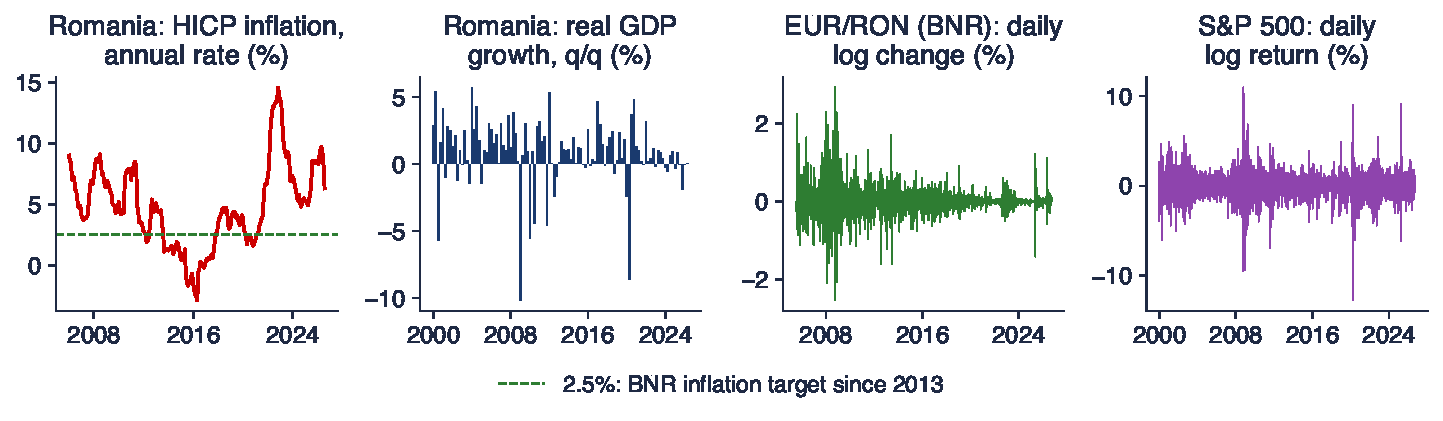
\includegraphics[width=0.97\textwidth,height=0.56\textheight,keepaspectratio]{ats_ch0_data_dashboard.pdf}
\end{center}
\vspace{-0.25cm}
\begin{itemize}
    \item Inflația IAPC în România, ianuarie 2006 -- august 2026: de la $\ensuremath{-}2{,}9\%$ (mai 2016) la $14{,}6\%$ (noiembrie 2022); ultima valoare $6{,}3\%$
    \item Creșterea PIB în România: 106 trimestre, minimum $\ensuremath{-}10{,}2\%$ în 2009Q1; zilnic: 5\,352 de observații EUR/RON și 6\,714 S\&P 500
\end{itemize}
\quantlet{ATS\_ch0\_dependence\_data}{\qlurl{ATS_ch0_dependence_data}}
\end{frame}

\begin{frame}{Interpretarea celor patru serii}
\itemsize{\small}
\begin{itemize}
    \item Inflația evoluează în cicluri lungi: ani peste linia de 2,5\% și ani sub ea
    \begin{itemize}
        \item Fiecare valoare lunară are unsprezece luni comune cu precedenta (rata anuală): suprapunerea mărește persistența
    \end{itemize}
    \item Creșterea PIB pare apropiată de un zgomot alb, cu excepția a două trimestre de criză
    \begin{itemize}
        \item Cu $T = 106$, două valori extreme domină varianța de selecție
    \end{itemize}
    \item EUR/RON și S\&P 500: volatility clustering (ani calmi, episoade de criză): dependență în momentul de ordinul doi
    \item Ce credeți? Care dintre cele patru serii are cea mai mare varianță de termen lung raportată la varianța ei?
\end{itemize}
\end{frame}

\begin{frame}{Autocorelația în șase serii}
\itemsize{\footnotesize}
\begin{center}
    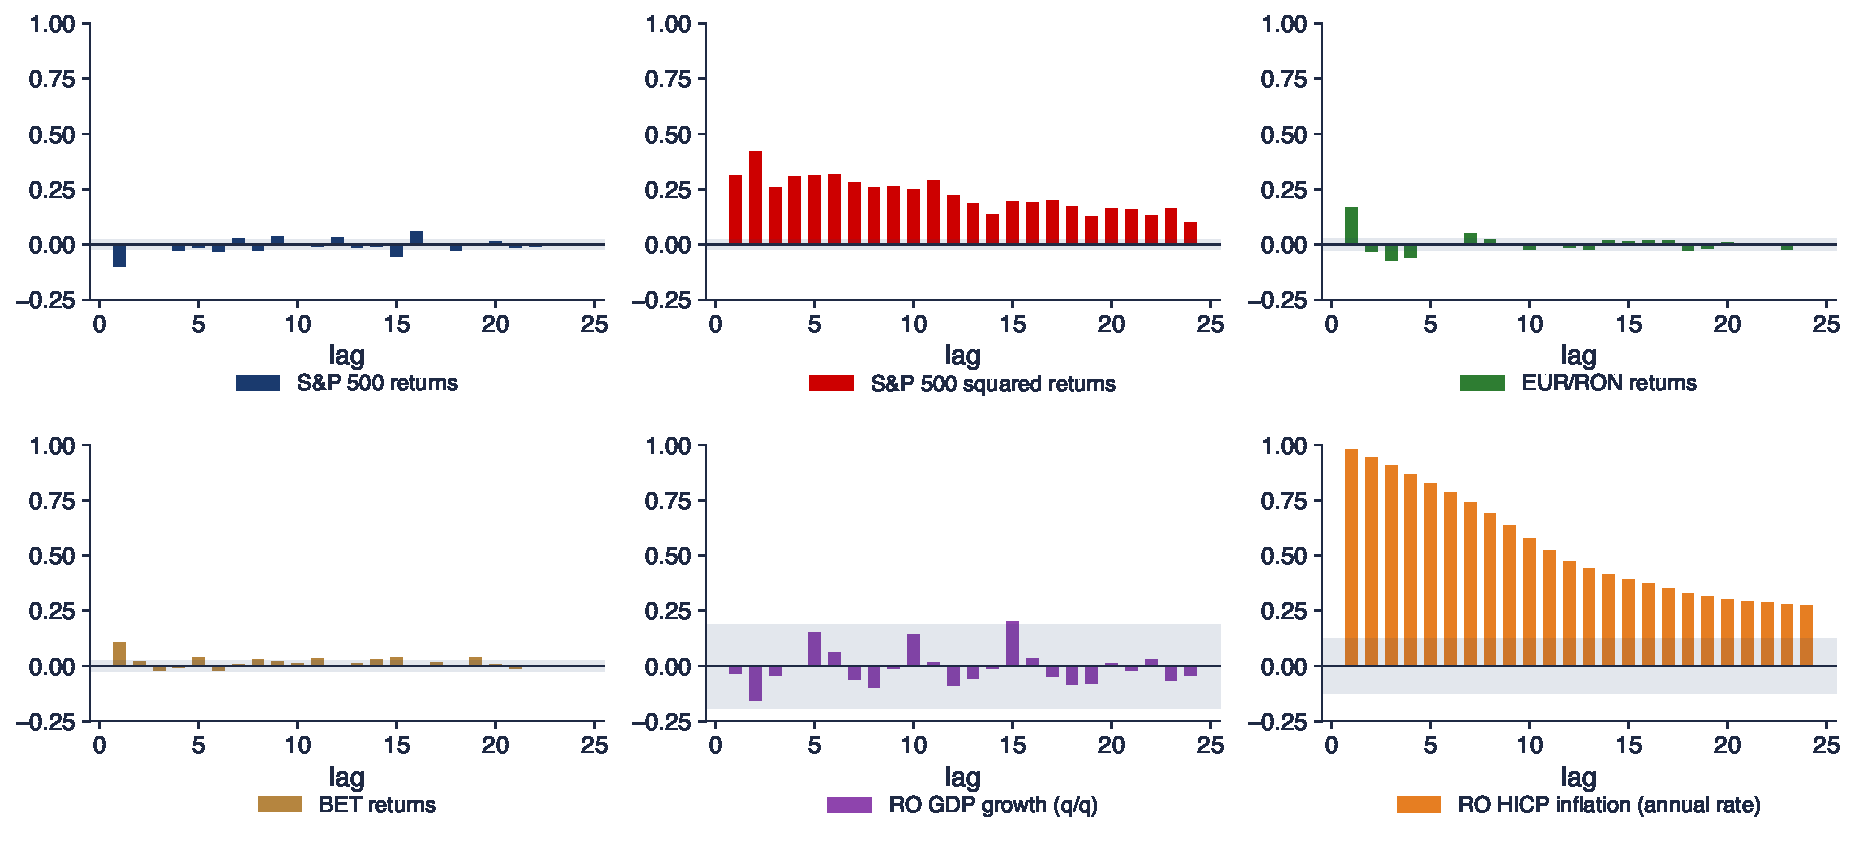
\includegraphics[width=0.97\textwidth,height=0.55\textheight,keepaspectratio]{ats_ch0_acf_panel.pdf}
\end{center}
\vspace{-0.25cm}
\begin{itemize}
    \item ACF de selecție, decalajele 1--24, cu banda $\pm 1{,}96/\sqrt{T}$ a ipotezei i.i.d.\ (hașurată)
    \item $\hat\rho_1$: S\&P 500 $\ensuremath{-}0{,}10$, pătrate $0{,}31$, EUR/RON $0{,}17$, BET $0{,}11$, PIB $\ensuremath{-}0{,}03$, inflație $0{,}98$
\end{itemize}
\quantlet{ATS\_ch0\_dependence\_data}{\qlurl{ATS_ch0_dependence_data}}
\end{frame}

\begin{frame}{Interpretarea autocorelațiilor}
\itemsize{\small}
\begin{itemize}
    \item Randamentele S\&P 500: $\hat\rho_1$ mic și negativ; pătratele: toate cele 24 de decalaje peste bandă, $\hat\rho_{12} = 0{,}22$
    \begin{itemize}
        \item Raportul dintre varianța de termen lung și varianță (lățimea Andrews): $0{,}8$ pentru randamente, $5{,}7$ pentru pătrate
    \end{itemize}
    \item BET și EUR/RON: $\hat\rho_1$ pozitiv (tranzacționare redusă, netezirea cursului de referință de către banca centrală)
    \begin{itemize}
        \item Rapoarte de $1{,}2$ și $1{,}1$: modeste, dar suficiente pentru a schimba o statistică $t$ aflată la limită
    \end{itemize}
    \item Inflația: $\hat\rho_1 = 0{,}98$ și un raport de $27{,}0$: o eroare standard naivă este de aproximativ cinci ori prea mică
    \item Restul capitolului: ce înseamnă aceste rapoarte, cum le estimăm și cînd estimările eșuează
\end{itemize}
\end{frame}

\begin{frame}{Recapitulare: harta recapitulării}
\itemsize{\small}
\begin{itemize}
    \item TSA a dat modelele; ATS are nevoie de inferența potrivită pentru date dependente
    \item Zgomotul alb nu înseamnă independență: randamentele GARCH sînt necorelate, pătratele lor nu
    \item Varianța de termen lung $\Omega = \sigma^2\theta(1)^2/\phi(1)^2$ leagă modelele ARMA de precizia unei medii de selecție
    \item În datele noastre, dependența variază de la neglijabilă (creșterea PIB) la extremă (inflația, pătratele randamentelor)
\end{itemize}
\end{frame}


%=============================================================================
\section{Asimptotică pentru date dependente}
%=============================================================================

\begin{frame}{Varianța unei medii în prezența dependenței}
\itemsize{\small}
\begin{itemize}
    \item Exact, pentru orice serie slab staționară:
    \begin{itemize}
        \item $\Var(\sqrt{T}\,\bar x) = \dfrac{1}{T}\sum_{t=1}^{T}\sum_{s=1}^{T}\gamma_{t-s} = \sum_{|j| < T}\Big(1 - \dfrac{|j|}{T}\Big)\gamma_j$
    \end{itemize}
    \item Dacă $\sum_j |\gamma_j| < \infty$ (convergență dominată):
    \begin{itemize}
        \item $\Var(\sqrt{T}\,\bar x) \to \Omega = \gamma_0 + 2\sum_{j\ge 1}\gamma_j = 2\pi f(0)$
    \end{itemize}
    \item Formula i.i.d.\ folosește doar $\gamma_0$; factorul de eroare este $\Omega/\gamma_0 = 1 + 2\sum_{j\ge1}\rho_j$
    \begin{itemize}
        \item Mărimea efectivă a eșantionului $T\gamma_0/\Omega$: un AR(1) cu $\phi = 0{,}9$ face ca 1000 de observații să valoreze cît aproximativ 53
    \end{itemize}
    \item Două întrebări: cînd are loc $\bar x \to \mu$ (LGN)? cînd este $\sqrt{T}(\bar x - \mu)/\sqrt{\Omega}$ asimptotic $N(0,1)$ (TLC)?
\end{itemize}
\end{frame}

\begin{frame}{Ergodicitate}
\itemsize{\footnotesize}
\begin{columns}[T]
\begin{column}{0.66\textwidth}
\begin{itemize}
    \item Un proces strict staționar $\{x_t\}$ este \textbf{ergodic} dacă orice eveniment invariant la translație are probabilitatea 0 sau 1
    \begin{itemize}
        \item Intuiție: o singură traiectorie lungă parcurge întreaga distribuție; mediile în timp sînt egale cu mediile pe ansamblu
    \end{itemize}
    \item \textbf{Teorema ergodică} \refBirkhoff: staționar, ergodic, $E|x_t| < \infty$ $\Rightarrow$ $\bar x \to E x_t$ aproape sigur
    \begin{itemize}
        \item Funcțiile de un număr finit de decalaje ale unui proces ergodic sînt ergodice: momente de selecție, autocovarianțe, MCMMP
    \end{itemize}
    \item Contraexemplu: $x_t = Z + \varepsilon_t$, cu $Z$ extras o singură dată: staționar, nu ergodic, $\bar x \to Z$
    \begin{itemize}
        \item Istoria unei singure economii este o singură extragere a lui $Z$: de aceea contează rupturile și regimurile (\atschlink{https://danpele.github.io/Advanced-Time-Series/RO/Cursuri/capitol2_rupturi_structurale_modele_neliniare.pdf}{capitolele 2}, \atschlink{https://danpele.github.io/Advanced-Time-Series/RO/Cursuri/capitol7_modele_schimbare_regim.pdf}{7})
    \end{itemize}
\end{itemize}
\end{column}
\begin{column}{0.30\textwidth}
\centering
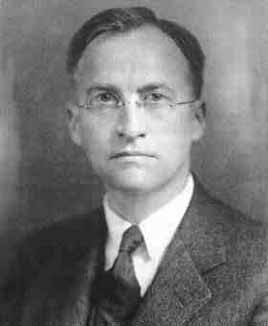
\includegraphics[height=0.42\textheight]{ch0_birkhoff_1910.jpg}\\[1mm]
\imgcap{George David Birkhoff (1884--1944)}
\imgcredit{https://commons.wikimedia.org/wiki/File:George_David_Birkhoff_1.jpg}{Foto: autor necunoscut (c.\ 1910); domeniu public; Wikimedia Commons}
\end{column}
\end{columns}
\end{frame}

\begin{frame}{Mixing: dependență care se stinge}
\itemsize{\footnotesize}
\begin{itemize}
    \item Coeficientul de mixing tare ($\alpha$) \refRosenblatt: $\alpha(m) = \sup_t\,\sup\{|P(A\cap B) - P(A)P(B)|: A \in \mathcal{F}_{-\infty}^{t}, B \in \mathcal{F}_{t+m}^{\infty}\}$
    \begin{itemize}
        \item $\alpha$-mixing: $\alpha(m) \to 0$; $\beta$-mixing și $\phi$-mixing sînt mai tari; mixing implică ergodicitate \refBradley
    \end{itemize}
    \item Ce modele sînt mixing?
    \begin{itemize}
        \item ARMA staționar cu inovații continue: $\beta$-mixing geometric \refMokkadem
        \item GARCH(1,1) strict staționar, volatilitate stochastică: $\beta$-mixing geometric \refCC
    \end{itemize}
    \item Ce modele nu sînt?
    \begin{itemize}
        \item Rădăcini unitare, memorie lungă cu $d > 0$ (\atschlink{https://danpele.github.io/Time-Series-Analysis/RO/Cursuri/capitol8_memorie_lunga_arfima.pdf}{TSA, Capitolul 8}), unele procese haotice deterministe: mixing nu are loc sau este prea lent pentru TLC standard
    \end{itemize}
    \item Coeficienții de mixing nu pot fi estimați dintr-o singură traiectorie: ipoteza se verifică prin model, nu se testează
\end{itemize}
\end{frame}

\begin{frame}{Legi ale numerelor mari pentru date dependente}
\itemsize{\small}
\begin{itemize}
    \item \textbf{Legea în $L^2$}: slab staționar cu $\gamma_j \to 0$ $\Rightarrow$ $E(\bar x - \mu)^2 \to 0$
    \begin{itemize}
        \item Demonstrație: $E(\bar x - \mu)^2 = T^{-1}\sum_{|j|<T}(1 - |j|/T)\gamma_j$, iar media Cesàro a lui $\gamma_j \to 0$ tinde la 0
    \end{itemize}
    \item \textbf{Legea ergodică} \refBirkhoff: convergență aproape sigură, doar $E|x_t| < \infty$, fără moment de ordinul doi
    \begin{itemize}
        \item Acoperă pătratele randamentelor unui GARCH cu moment de ordinul patru infinit: mediile converg, dar TLC poate să nu aibă loc
    \end{itemize}
    \item \textbf{Mixingale și dependență near-epoch}: variantele folosite în teoria econometrică pentru funcții de procese mixing \refHamilton
    \item Consistența (LGN) se obține ușor; erorile standard valide (TLC plus un $\hat\Omega$ consistent) sînt partea dificilă
\end{itemize}
\end{frame}

\begin{frame}{Diferențele de martingală și teorema limită centrală}
\itemsize{\small}
\begin{itemize}
    \item $\{u_t\}$ este o \textbf{secvență de diferențe de martingală} (MDS) dacă $E(u_t \mid \mathcal{F}_{t-1}) = 0$
    \begin{itemize}
        \item Necorelat cu orice funcție de trecut, dar poate fi condiționat heteroscedastic: randamente GARCH, scoruri ale unei verosimilități corecte, erorile prognozelor optime pe un pas
    \end{itemize}
    \item \textbf{TLC pentru MDS} \refBillingsley: MDS staționară, ergodică, cu $E u_t^2 = \sigma^2 < \infty$ $\Rightarrow$ $\sqrt{T}\,\bar u \to_d N(0, \sigma^2)$
    \begin{itemize}
        \item MDS nestaționare: condiții de tip Lindeberg \refBrown
        \item Aici $\Omega = \gamma_0$: nu este nevoie de corecție pentru autocorelație, doar de erori robuste la heteroscedasticitate White (1980) \refWhiteH
    \end{itemize}
    \item Erorile prognozelor pe $h$ pași, suprapuse, nu sînt MDS: urmează un MA$(h-1)$ (secțiunea „Observații suprapuse”)
\end{itemize}
\end{frame}

\begin{frame}{Teoreme limită centrală dincolo de diferențele de martingală}
\itemsize{\footnotesize}
\begin{itemize}
    \item \textbf{TLC pentru procese mixing} \refIbragimov: staționar, $E|x_t|^{2+\delta} < \infty$, $\sum_m \alpha(m)^{\delta/(2+\delta)} < \infty$, $\Omega > 0$ $\Rightarrow$ $\sqrt{T}(\bar x - \mu) \to_d N(0, \Omega)$
    \begin{itemize}
        \item Compromis: mai multe momente permit un mixing mai lent; prima TLC sub mixing tare este \refRosenblatt
    \end{itemize}
    \item \textbf{Procese liniare} \refPS: $x_t - \mu = \sum\psi_j\varepsilon_{t-j}$ cu $\varepsilon_t$ i.i.d.\ sau MDS și $\sum j|\psi_j| < \infty$
    \begin{itemize}
        \item Beveridge--Nelson: $\psi(L) = \psi(1) - (1-L)\tilde\psi(L)$, deci $\sqrt{T}(\bar x - \mu) = \psi(1)\sqrt{T}\bar\varepsilon + o_p(1)$, de unde $\Omega = \sigma^2\psi(1)^2$
    \end{itemize}
    \item Versiunile funcționale (principii de invarianță) dau limitele de tip mișcare browniană din teoria rădăcinilor unitare și din teoria fixed-$b$
    \item Toate trei cer $0 < \Omega < \infty$: rădăcinile unitare dau $\Omega = \infty$, supradiferențierea dă $\Omega = 0$
\end{itemize}
\end{frame}

\begin{frame}{Cîtă informație elimină dependența?}
\itemsize{\footnotesize}
\begin{center}
    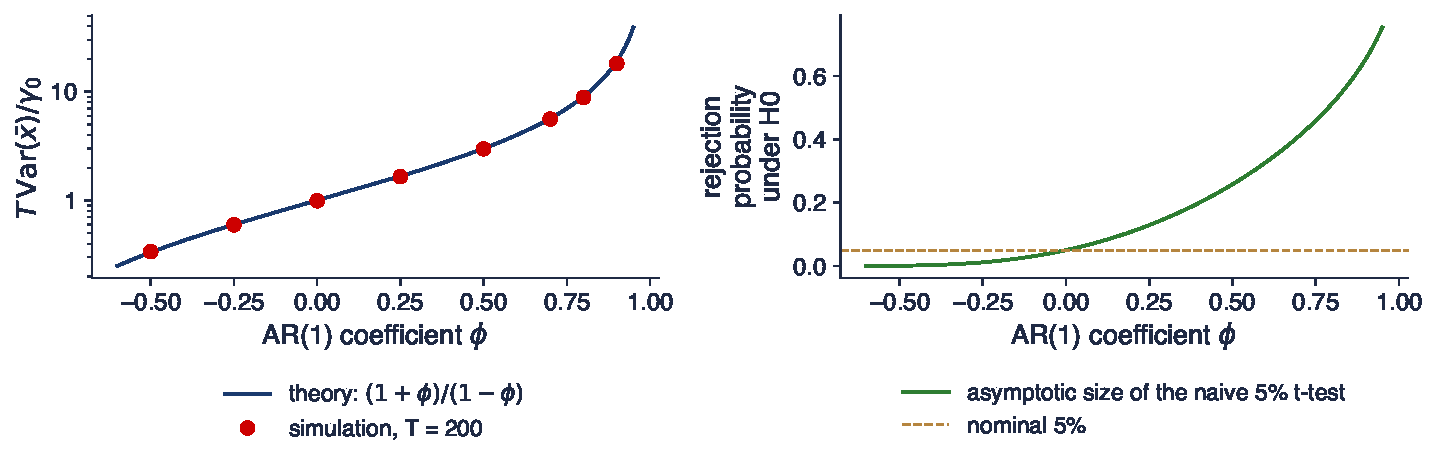
\includegraphics[width=0.97\textwidth,height=0.56\textheight,keepaspectratio]{ats_ch0_lrv_ar1.pdf}
\end{center}
\vspace{-0.25cm}
\begin{itemize}
    \item Stînga: $T\Var(\bar x)/\gamma_0$ pentru un AR(1), teoria $(1+\phi)/(1-\phi)$ și 20\,000 de simulări cu $T = 200$; dreapta: mărimea asimptotică a testului naiv de 5\%, $2[1 - \Phi(1{,}96/\sqrt{(1+\phi)/(1-\phi)})]$
\end{itemize}
\quantlet{ATS\_ch0\_long\_run\_variance}{\qlurl{ATS_ch0_long_run_variance}}
\end{frame}

\begin{frame}{Interpretarea creșterii varianței}
\itemsize{\small}
\begin{itemize}
    \item $\phi = 0,5$: factorul este $3$ (simulat $2{,}98$); $\phi = 0,9$: $19$ (simulat $18{,}1$; factorul $1 - |j|/T$ al eșantionului finit îl reduce)
    \begin{itemize}
        \item Testul naiv respinge o ipoteză $H_0$ adevărată cu probabilitatea $15\%$ la $\phi = 0,3$, $26\%$ la $0,5$ și $65\%$ la $0,9$
    \end{itemize}
    \item Dependența negativă acționează invers: $\phi = -0,5$ dă un factor de $0{,}33$, deci un test naiv conservator
    \begin{itemize}
        \item Media randamentelor S\&P 500 este un exemplu: eroarea ei standard HAC este mai mică decît cea naivă
    \end{itemize}
    \item Intervalele de încredere moștenesc factorul: un interval naiv de 95\% acoperă $\mu$ doar în aproximativ $74\%$ din cazuri la $\phi = 0,5$
\end{itemize}
\end{frame}

\begin{frame}{Regresia cu erori dependente}
\itemsize{\small}
\begin{itemize}
    \item $y_t = x_t'\beta + u_t$, $E(x_t u_t) = 0$; sub o TLC pentru $x_t u_t$:
    \begin{itemize}
        \item $\sqrt{T}(\hat\beta - \beta) \to_d N\big(0,\; Q^{-1}\Omega_{xu} Q^{-1}\big)$, $\quad Q = E(x_t x_t'),\quad \Omega_{xu} = \sum_{j}E(x_t u_t u_{t-j} x_{t-j}')$
    \end{itemize}
    \item Panta scalară, $x_t$ și $u_t$ serii staționare independente: factorul de eroare este
    \begin{itemize}
        \item $\Omega_{xu}/(\gamma_{x,0}\gamma_{u,0}) = 1 + 2\sum_{j\ge 1}\rho_{x}(j)\rho_{u}(j)$
        \item Atît regresorul, cît și eroarea trebuie să fie persistente pentru o distorsiune mare: un predictor persistent cu erori persistente este cazul cel mai rău
    \end{itemize}
    \item Forma sandwich $\hat Q^{-1}\hat\Omega_{xu}\hat Q^{-1}$, cu o estimare prin nucleu a lui $\Omega_{xu}$, este matricea de covarianță Newey--West \refNW
\end{itemize}
\end{frame}

\begin{frame}{Recapitulare: asimptotică pentru date dependente}
\itemsize{\small}
\begin{itemize}
    \item $\Var(\sqrt{T}\bar x) \to \Omega = \sum_j\gamma_j = 2\pi f(0)$; formula i.i.d.\ păstrează doar $\gamma_0$
    \item Ergodicitatea dă LGN; mixing sau structura de martingală, plus momente, dau TLC
    \item Pentru o MDS, $\Omega = \gamma_0$: erorile robuste la heteroscedasticitate sînt suficiente
    \item Persistența pozitivă face ca testele naive să respingă prea des; persistența negativă le face conservatoare
\end{itemize}
\end{frame}


%=============================================================================
\section{Estimarea HAC}
%=============================================================================

\begin{frame}{Estimarea varianței de termen lung}
\itemsize{\small}
\begin{itemize}
    \item Înlocuirea tuturor autocovarianțelor de selecție: $\sum_{|j|<T}\hat\gamma_j = 0$ identic (date centrate): inutil
    \begin{itemize}
        \item Autocovarianțele $\hat\gamma_j$ de ordin mare folosesc puține perechi și sînt zgomot
    \end{itemize}
    \item \textbf{Estimatorul prin nucleu}: $\hat\Omega = \sum_{|j|<T} k(j/S)\,\hat\gamma_j$, cu $k(0) = 1$, $k$ descrescătoare în $|x|$
    \begin{itemize}
        \item Echivalent, o periodogramă netezită la frecvența 0: $\hat\Omega = 2\pi\hat f(0)$ \refSS
    \end{itemize}
    \item Consistență: $S \to \infty$ și $S/T \to 0$ (Andrews 1991, sub condiții de mixing și de momente) \refAndrews
    \begin{itemize}
        \item Deplasarea vine din decalajele subponderate, varianța din cele incluse: $S$ echilibrează cele două
    \end{itemize}
    \item Un estimator de varianță trebuie să fie nenegativ: nu orice nucleu garantează acest lucru
\end{itemize}
\end{frame}

\begin{frame}{Studiu de caz: Newey și West (1987)}
\itemsize{\footnotesize}
\begin{itemize}
    \item \refNW, Econometrica 55(3): nucleul Bartlett $k(x) = 1 - |x|$ pentru $|x| \le 1$, cu $L$ decalaje:
    \begin{itemize}
        \item $\hat\Omega_{NW} = \hat\Gamma_0 + \sum_{j=1}^{L}\Big(1 - \dfrac{j}{L+1}\Big)\big(\hat\Gamma_j + \hat\Gamma_j'\big)$, $\quad\hat\Gamma_j = T^{-1}\sum_{t>j}\hat h_t\hat h_{t-j}'$, $\hat h_t = x_t\hat u_t$
    \end{itemize}
    \item \textbf{Pozitiv semidefinit prin construcție}: ponderile Bartlett sînt autocovarianțele unei sume mobile
    \begin{itemize}
        \item $\hat\Omega_{NW}$ este egal (pînă la efectele de capăt) cu $\frac{1}{(L+1)T}\sum_t\big(\sum_{i=0}^{L}\hat h_{t-i}\big)\big(\sum_{i=0}^{L}\hat h_{t-i}\big)'$: o sumă de produse exterioare
        \item Perspectiva spectrală: fereastra Bartlett (Fejér) este nenegativă la orice frecvență
    \end{itemize}
    \item Consistență cu $L \to \infty$, $L = o(T^{1/4})$ în lucrarea originală; Andrews (1991) rafinează ratele
    \item O pagină de algebră, astăzi eroarea standard „robustă” implicită în orice pachet econometric
\end{itemize}
\end{frame}

\begin{frame}{Un nucleu trunchiat poate da o varianță negativă}
\itemsize{\small}
\begin{itemize}
    \item Nucleul trunchiat (uniform): $k(x) = 1$ pentru $|x| \le 1$: $\hat\Omega = \hat\gamma_0 + 2\sum_{j=1}^{L}\hat\gamma_j$ (folosit de \refHH{} pentru prognozele suprapuse)
    \begin{itemize}
        \item Exact corect cînd $\gamma_j = 0$ pentru $j > L$, de exemplu o eroare de prognoză MA$(h-1)$ cu $L = h - 1$
    \end{itemize}
    \item Zece observații cu semn alternant, $(1, -1, 1, -1, 1, -1, 1, -1, 2, -2)$: $\hat\gamma_0 = 1{,}6$, $\hat\gamma_1 = \ensuremath{-}1{,}3$, $\hat\gamma_2 = 1{,}0$
    \begin{itemize}
        \item Trunchiat, $L = 1$: $\hat\gamma_0 + 2\hat\gamma_1 = \ensuremath{-}1{,}0 < 0$
        \item Bartlett, $L = 1$: $\hat\gamma_0 + \hat\gamma_1 = 0{,}3 > 0$
    \end{itemize}
    \item Lecția: o varianță negativă nu este un accident numeric; este o proprietate a nucleului (Seminarul 0, A3--A4)
\end{itemize}
\end{frame}

\begin{frame}{Nucleele}
\itemsize{\footnotesize}
\begin{center}
    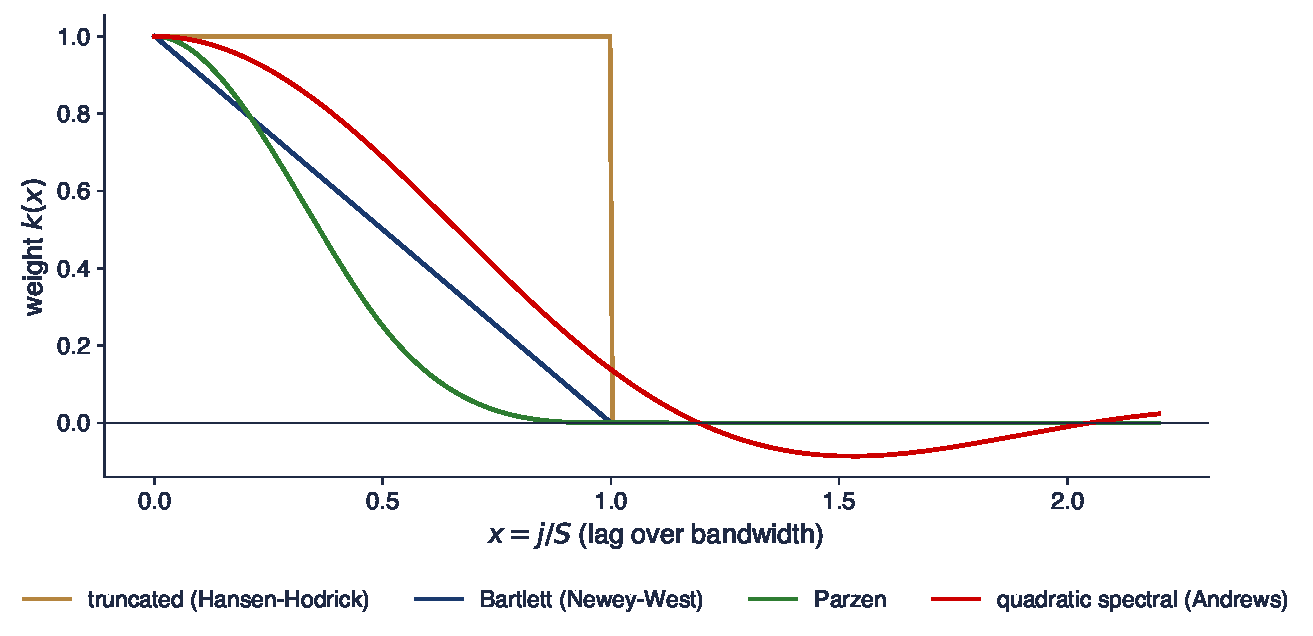
\includegraphics[width=0.97\textwidth,height=0.52\textheight,keepaspectratio]{ats_ch0_kernels.pdf}
\end{center}
\vspace{-0.25cm}
\begin{itemize}
    \item Parzen: $1 - 6x^2 + 6|x|^3$ ($|x| \le 1/2$), $2(1-|x|)^3$ ($1/2 < |x| \le 1$); QS: $\frac{25}{12\pi^2x^2}\big[\frac{\sin(6\pi x/5)}{6\pi x/5} - \cos(6\pi x/5)\big]$, toate decalajele
\end{itemize}
\quantlet{ATS\_ch0\_long\_run\_variance}{\qlurl{ATS_ch0_long_run_variance}}
\end{frame}

\begin{frame}{Interpretarea nucleelor}
\itemsize{\small}
\begin{itemize}
    \item Bartlett, Parzen și QS au ferestre spectrale nenegative: întotdeauna $\hat\Omega \ge 0$
    \begin{itemize}
        \item QS are ponderi negative mici (minimum $\ensuremath{-}0{,}086$), dar rămîne pozitiv semidefinit
    \end{itemize}
    \item Ordinul nucleului $q$: $1 - k(x) \sim c|x|^q$ lîngă 0; Bartlett $q = 1$, Parzen și QS $q = 2$
    \begin{itemize}
        \item Deplasare $O(S^{-q})$, varianță $O(S/T)$: $S$ optim $\propto T^{1/(2q+1)}$, adică $T^{1/3}$ (Bartlett) și $T^{1/5}$ (QS)
    \end{itemize}
    \item \refAndrews: QS minimizează eroarea pătratică medie asimptotică printre nucleele cu estimări nenegative
\end{itemize}
\end{frame}

\begin{frame}{Studiu de caz: Andrews (1991) și alegerea lățimii de bandă}
\itemsize{\footnotesize}
\begin{itemize}
    \item Lățimea optimă în sensul erorii pătratice medii: $S^* = c_k\,(\alpha(q)\,T)^{1/(2q+1)}$, cu $\alpha(q)$ dependent de spectrul necunoscut \refAndrews
    \begin{itemize}
        \item Bartlett: $S^* = 1{,}1447(\hat\alpha(1)T)^{1/3}$; Parzen: $2{,}6614(\hat\alpha(2)T)^{1/5}$; QS: $1{,}3221(\hat\alpha(2)T)^{1/5}$
    \end{itemize}
    \item \textbf{Înlocuirea AR(1)}: estimăm $\hat\rho$ pe $\hat h_t$, apoi
    \begin{itemize}
        \item $\hat\alpha(1) = \dfrac{4\hat\rho^2}{(1-\hat\rho)^2(1+\hat\rho)^2}$, $\qquad \hat\alpha(2) = \dfrac{4\hat\rho^2}{(1-\hat\rho)^4}$
    \end{itemize}
    \item Alternative
    \begin{itemize}
        \item Regula practică Newey--West $L = \lfloor 4(T/100)^{2/9}\rfloor$ și selecția lor automată neparametrică \refNWb
        \item Prealbirea cu un VAR(1), apoi recolorarea \refAM: mai puțină deplasare pentru seriile persistente
    \end{itemize}
    \item Criteriul erorii pătratice medii vizează $\hat\Omega$, nu testul: de aici provin distorsiunile de mărime (secțiunile următoare)
\end{itemize}
\end{frame}

\begin{frame}{Erorile standard HAC în funcție de lățimea de bandă}
\itemsize{\footnotesize}
\begin{center}
    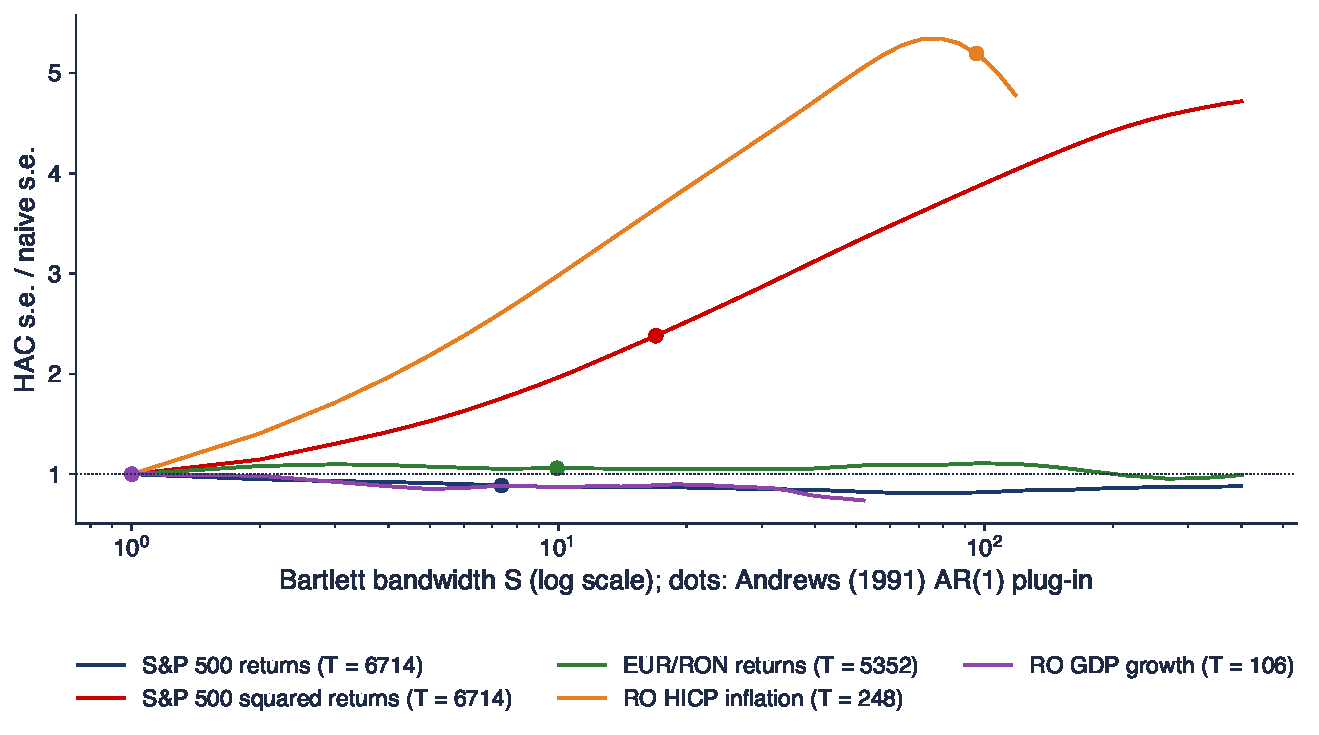
\includegraphics[width=0.97\textwidth,height=0.56\textheight,keepaspectratio]{ats_ch0_hac_bandwidth.pdf}
\end{center}
\vspace{-0.25cm}
\begin{itemize}
    \item Raportul dintre eroarea standard HAC Bartlett a mediei și cea naivă, $S$ de la 1 la $\min(400, T/2)$; puncte: înlocuirea AR(1) Andrews
\end{itemize}
\quantlet{ATS\_ch0\_hac}{\qlurl{ATS_ch0_hac}}
\end{frame}

\begin{frame}{Interpretarea traiectoriilor în funcție de lățimea de bandă}
\itemsize{\small}
\begin{itemize}
    \item Pătratele randamentelor S\&P 500: raport $2{,}04$ cu regula practică ($S = 11$), $2{,}38$ cu Andrews ($S = 17$), în creștere pînă la $4{,}72$ la $S = 400$
    \begin{itemize}
        \item Fără platou: înlocuirea AR(1) nu surprinde scăderea lentă a autocorelației volatilității (memorie lungă, \atschlink{https://danpele.github.io/Advanced-Time-Series/RO/Cursuri/capitol10_memorie_lunga_rough_volatility.pdf}{Capitolul 10})
    \end{itemize}
    \item Inflația în România: $2{,}18$ cu regula practică, $5{,}19$ cu Andrews ($S = 96$ luni)
    \begin{itemize}
        \item Regula practică ignoră datele: la $T$ fix dă același $S$ pentru un zgomot alb și pentru o rădăcină aproape unitară
    \end{itemize}
    \item Randamentele S\&P 500: raport sub 1 la orice $S$ ($\hat\rho_1$ negativ); EUR/RON: aproape constant, în jur de $1{,}06$
\end{itemize}
\end{frame}

\begin{frame}{Asimptotica fixed-$b$}
\itemsize{\small}
\begin{itemize}
    \item Teoria standard: $S/T \to 0$, $\hat\Omega \to_p \Omega$, statistica $t$ este $N(0,1)$: eroarea de selecție a lui $\hat\Omega$ este ignorată
    \begin{itemize}
        \item În eșantioane de 100--300 de observații, $\hat\Omega$ este zgomotos și deplasat în jos: valorile critice normale sînt prea mici
    \end{itemize}
    \item \textbf{Fixed-$b$} \refKVB, \refKVb, \refKV: păstrăm $b = S/T$ fix cînd $T \to \infty$
    \begin{itemize}
        \item $\hat\Omega/\Omega \to_d Q_k(b)$, o funcțională a unei punți browniene $\tilde W(r) = W(r) - rW(1)$; $t \to_d W(1)/\sqrt{Q_k(b)}$
        \item Nestandard, dar pivotal: valorile critice depind doar de nucleu și de $b$
    \end{itemize}
    \item Teoria de ordin superior: valorile critice fixed-$b$ elimină termenul principal al distorsiunii de mărime din aproximarea normală \refSPJ
\end{itemize}
\end{frame}

\begin{frame}{Valorile critice fixed-$b$}
\itemsize{\footnotesize}
\begin{center}
    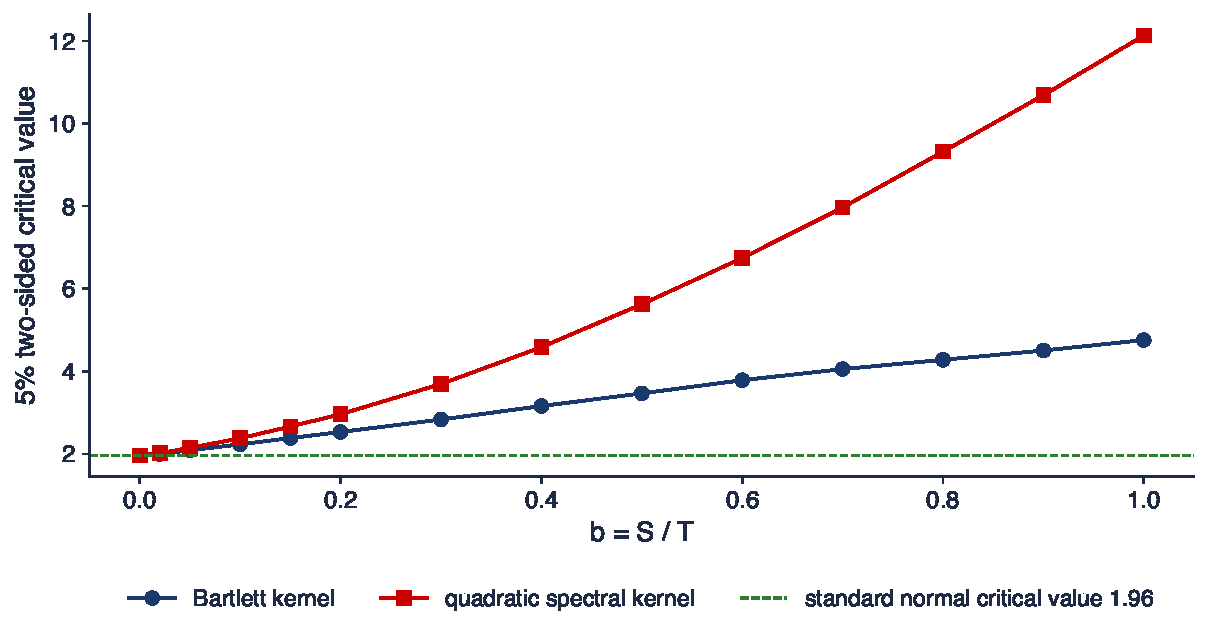
\includegraphics[width=0.97\textwidth,height=0.55\textheight,keepaspectratio]{ats_ch0_fixed_b.pdf}
\end{center}
\vspace{-0.25cm}
\begin{itemize}
    \item Valori critice bilaterale de 5\% ale testului $t$ pentru medie cu $S = bT$, simulate (20\,000 de eșantioane normale i.i.d., $T = 500$)
\end{itemize}
\quantlet{ATS\_ch0\_hac}{\qlurl{ATS_ch0_hac}}
\end{frame}

\begin{frame}{Interpretarea valorilor critice fixed-$b$}
\itemsize{\small}
\begin{itemize}
    \item Bartlett: $2{,}23$ la $b = 0,1$, $3{,}47$ la $b = 0,5$, $4{,}76$ la $b = 1$ (statistica Kiefer--Vogelsang--Bunzel)
    \begin{itemize}
        \item Apropiate de aproximarea cubică raportată de \refKV{} pentru nucleul Bartlett
    \end{itemize}
    \item QS: $2{,}38$ la $b = 0,1$ și $5{,}62$ la $b = 0,5$: QS cu $b$ mare este foarte zgomotos
    \item $b$ mai mare: deplasare mai mică a lui $\hat\Omega$, varianță mai mare, compensată de o valoare critică mai mare: mărime mai bună, putere mai mică
    \item Ce credeți? De ce tinde valoarea critică la 1,96 cînd $b \to 0$?
\end{itemize}
\end{frame}

\begin{frame}{Recomandări practice: Lazarus, Lewis, Stock și Watson (2018)}
\itemsize{\footnotesize}
\begin{itemize}
    \item \refLLSW{} aleg lățimea de bandă pentru \emph{test}: o frontieră mărime--putere, nu eroarea pătratică medie a lui $\hat\Omega$
    \begin{itemize}
        \item Newey--West cu $S = 1{,}3\sqrt{T}$ și valori critice fixed-$b$
        \item Cosinus cu ponderi egale (EWC): $\hat\Omega = \nu^{-1}\sum_{j=1}^{\nu}\hat\Lambda_j^2$, $\hat\Lambda_j = \sqrt{2/T}\sum_t \cos[\pi j(t - 1/2)/T]\hat h_t$, $\nu = 0{,}4T^{2/3}$, valori critice Student $t_\nu$
    \end{itemize}
    \item Compromisul mărime--putere este inevitabil: \refLLS{} dau frontiera pentru testele cu nucleu
    \item Serii foarte persistente ($\phi$ aproape de 1): nicio regulă cu nucleu sau EWC nu este fiabilă; \refMuller{} propune teste valide sub dependență local-unitară
    \item Acestea sînt opțiunile implicite ale cursului începînd cu \atschlink{https://danpele.github.io/Advanced-Time-Series/RO/Cursuri/capitol1_evaluarea_prognozelor.pdf}{Capitolul 1}
\end{itemize}
\end{frame}

\begin{frame}{Recapitulare: estimarea HAC}
\itemsize{\small}
\begin{itemize}
    \item Estimatorii prin nucleu subponderează decalajele îndepărtate; Bartlett (Newey--West), Parzen și QS sînt întotdeauna nenegativi; nucleul trunchiat nu este
    \item Lățimile Andrews (1991) sînt optime pentru eroarea pătratică medie a lui $\hat\Omega$ și se adaptează persistenței; regula practică nu
    \item Valorile critice fixed-$b$ țin cont de zgomotul din $\hat\Omega$; LLSW: NW cu $S = 1{,}3\sqrt{T}$ sau EWC cu $\nu = 0{,}4T^{2/3}$
\end{itemize}
\end{frame}


%=============================================================================
\section{Distorsiuni de mărime: un studiu Monte Carlo}
%=============================================================================

\begin{frame}{Planul Monte Carlo}
\itemsize{\small}
\begin{itemize}
    \item DGP: $x_t = \phi x_{t-1} + \varepsilon_t$, $\varepsilon_t \sim N(0,1)$ i.i.d., 200 de valori inițiale eliminate; $H_0: \mu = 0$ este adevărată
    \begin{itemize}
        \item $\phi \in \{0; 0,3; 0,5; 0,7; 0,9\}$, $T \in \{100; 400\}$; 5\,000 de replicări (1\,000 pentru bootstrap, cu cîte 399 de reeșantionări); sămînța 2026
    \end{itemize}
    \item Șapte teste la nivelul nominal de 5\%
    \begin{itemize}
        \item naiv i.i.d.; NW cu regula practică; NW și QS cu lățimea Andrews AR(1) (valori critice normale)
        \item NW cu $S = 1{,}3\sqrt{T}$ și valori fixed-$b$; EWC cu $t_\nu$; bootstrap circular pe blocuri cu lungimea Politis--White
    \end{itemize}
    \item Eroarea standard Monte Carlo a unei rate de respingere $p$: $\sqrt{p(1-p)/R}$, aproximativ $0,3$ pp la $p = 5\%$ și $R = 5000$
    \item Același plan ca în secțiunile Monte Carlo din \refAndrews{} și \refKV: date AR(1), rate de respingere sub ipoteza nulă
\end{itemize}
\end{frame}

\begin{frame}{Mărimea a șapte teste sub dependență AR(1)}
\itemsize{\footnotesize}
\begin{center}
    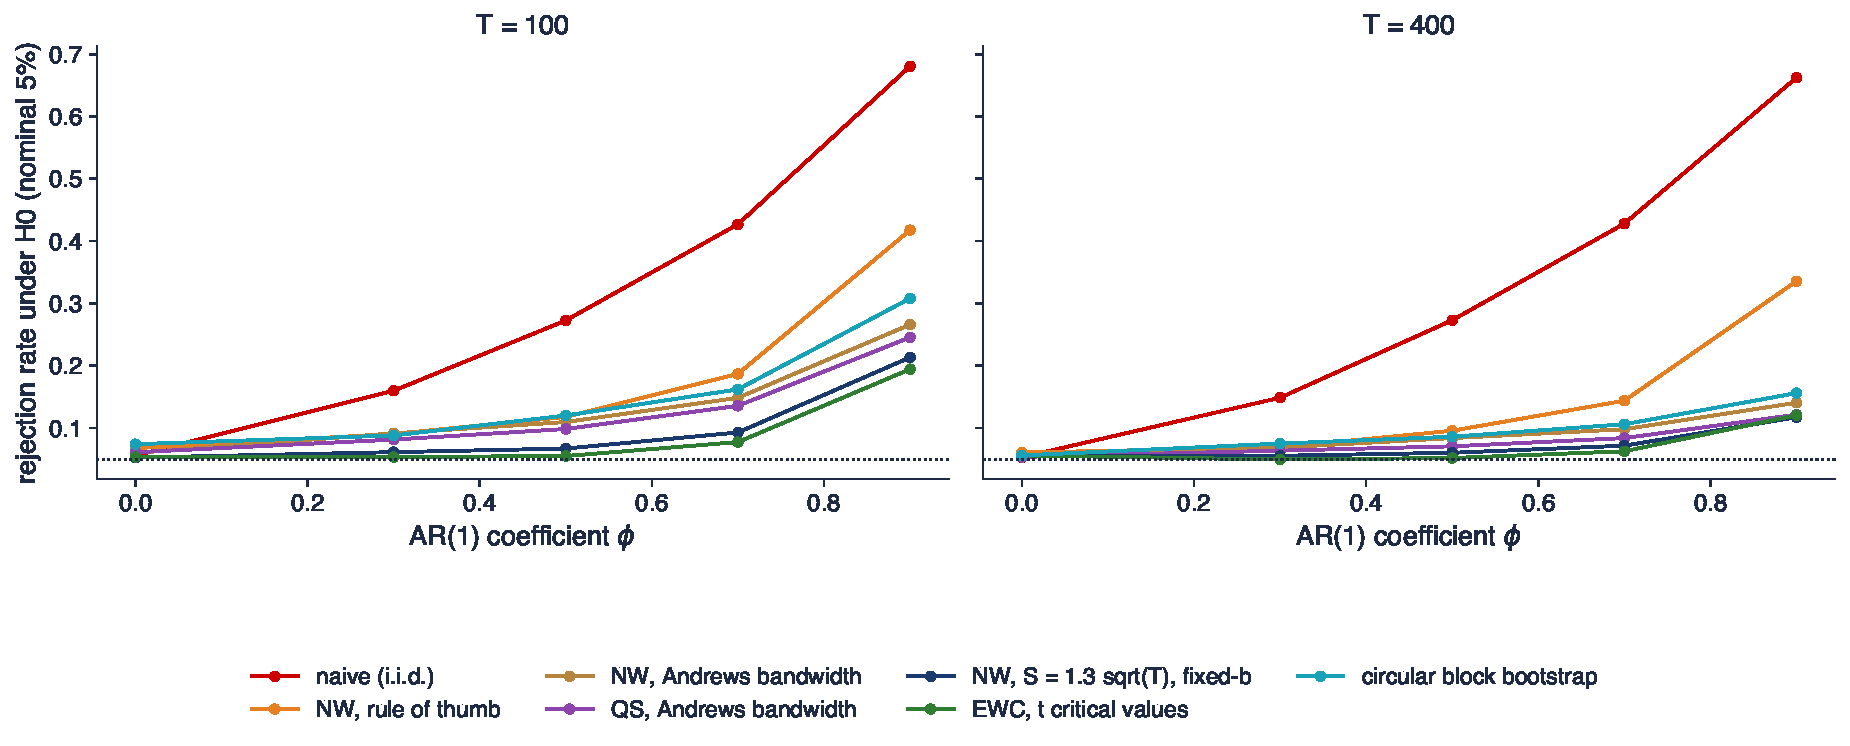
\includegraphics[width=0.97\textwidth,height=0.58\textheight,keepaspectratio]{ats_ch0_mc_size.pdf}
\end{center}
\vspace{-0.25cm}
\begin{itemize}
    \item Rata de respingere a ipotezei $H_0: \mu = 0$ (adevărată) în funcție de $\phi$; linia punctată: 5\%
\end{itemize}
\quantlet{ATS\_ch0\_size\_monte\_carlo}{\qlurl{ATS_ch0_size_monte_carlo}}
\end{frame}

\begin{frame}{Mărimea în cifre (\%)}
\itemsize{\footnotesize}
\begin{center}
\footnotesize
\begin{tabular}{lrrrrrr}
\toprule
& \multicolumn{3}{c}{$T = 100$} & \multicolumn{3}{c}{$T = 400$} \\
Testul & $\phi = 0$ & $0{,}5$ & $0{,}9$ & $\phi = 0$ & $0{,}5$ & $0{,}9$ \\
\midrule
naiv i.i.d. & 5{,}6 & 27{,}3 & 68{,}1 & 5{,}3 & 27{,}3 & 66{,}2 \\
NW, regula practică & 6{,}8 & 11{,}8 & 41{,}8 & 6{,}1 & 9{,}6 & 33{,}6 \\
NW, Andrews & 6{,}0 & 11{,}0 & 26{,}6 & 5{,}3 & 8{,}4 & 14{,}1 \\
QS, Andrews & 6{,}1 & 9{,}8 & 24{,}6 & 5{,}4 & 7{,}1 & 12{,}1 \\
NW, $1{,}3\sqrt{T}$, fixed-$b$ & 5{,}2 & 6{,}7 & 21{,}3 & 5{,}6 & 6{,}0 & 11{,}7 \\
EWC, $t_\nu$ & 5{,}3 & 5{,}5 & 19{,}4 & 5{,}6 & 5{,}2 & 12{,}1 \\
bootstrap circular pe blocuri & 7{,}4 & 12{,}0 & 30{,}8 & 5{,}6 & 8{,}6 & 15{,}6 \\
\bottomrule
\end{tabular}
\end{center}
\begin{itemize}
    \item Erori standard Monte Carlo: aproximativ 0,3 pp în jurul valorii de 5\%, aproximativ 0,7 pp în jurul valorii de 30\% (rîndurile bootstrap: de aproximativ două ori mai mari)
\end{itemize}
\end{frame}

\begin{frame}{Interpretarea studiului Monte Carlo}
\itemsize{\footnotesize}
\begin{itemize}
    \item Testul naiv: $27{,}3\%$ la $\phi = 0,5$ și $68{,}1\%$ la $\phi = 0,9$; mai multe date nu ajută ($66{,}2\%$ la $T = 400$)
    \begin{itemize}
        \item Distorsiunea este o proprietate a estimatorului, nu a mărimii eșantionului
    \end{itemize}
    \item NW cu regula practică: $41{,}8\%$ la $\phi = 0,9$, $T = 100$; lățimile Andrews reduc excesul la jumătate; fixed-$b$ și EWC se apropie cel mai mult ($21{,}3\%$, $19{,}4\%$)
    \begin{itemize}
        \item La $T = 400$ și $\phi = 0,5$: $6{,}0\%$ și $5{,}2\%$, practic exacte
    \end{itemize}
    \item Bootstrap pe blocuri nu rezolvă totul: $30{,}8\%$ la $\phi = 0,9$, $T = 100$, între NW și fixed-$b$
    \item Seria noastră de inflație are $\hat\rho_1 = 0{,}98$: în afara domeniului în care vreunul dintre aceste teste este fiabil (mini-studiul de caz AI)
\end{itemize}
\end{frame}

\begin{frame}{Recapitulare: distorsiunile de mărime}
\itemsize{\small}
\begin{itemize}
    \item Raportați întotdeauna mărimea efectivă a procedurii folosite, la persistența datelor voastre
    \item NW fixed-$b$ și EWC (LLSW 2018) domină alegerile clasice în privința mărimii, cu un cost modest în putere
    \item Un studiu Monte Carlo este un experiment: fixați sămînța, raportați $R$ și eroarea standard Monte Carlo
\end{itemize}
\end{frame}


%=============================================================================
\section{Bootstrap pentru date dependente}
%=============================================================================

\begin{frame}{Eșecul bootstrap-ului i.i.d.}
\itemsize{\footnotesize}
\begin{columns}[T]
\begin{column}{0.66\textwidth}
\begin{itemize}
    \item Bootstrap Efron \refEfron{} reeșantionează observații individuale: dependența este distrusă
    \begin{itemize}
        \item $\Var^*(\sqrt{T}\bar x^*) = \hat\gamma_0$, nu $\Omega$: bootstrap i.i.d.\ reproduce eroarea standard naivă
    \end{itemize}
    \item \refSingh: chiar pentru date $m$-dependente, bootstrap i.i.d.\ pentru medie este inconsistent
    \begin{itemize}
        \item Ideea bootstrap pe blocuri: reeșantionăm blocuri suficient de lungi pentru a păstra dependența în interiorul lor
    \end{itemize}
    \item Prețul: dependența de la granițele blocurilor se pierde, iar lungimea blocului devine un parametru de reglaj
\end{itemize}
\end{column}
\begin{column}{0.30\textwidth}
\centering
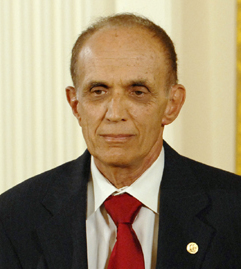
\includegraphics[height=0.40\textheight]{ch0_efron_2007.jpg}\\[1mm]
\imgcap{Bradley Efron (2007)}
\imgcredit{https://commons.wikimedia.org/wiki/File:Bradley_Efron_National_Medal_of_Science_2007_(cropped).jpg}{Foto: Ryan K. Morris, NSTMF (2007); domeniu public; Wikimedia Commons}
\end{column}
\end{columns}
\end{frame}

\begin{frame}{Studiu de caz: bootstrap pe blocuri mobile, Künsch (1989)}
\itemsize{\footnotesize}
\begin{columns}[T]
\begin{column}{0.64\textwidth}
\begin{itemize}
    \item \refKunsch: blocurile $B_i = (x_i, \dots, x_{i+l-1})$, $i = 1, \dots, T - l + 1$
    \begin{itemize}
        \item Extragem $k = \lceil T/l\rceil$ blocuri cu întoarcere, le concatenăm și păstrăm primele $T$ valori
    \end{itemize}
    \item Consistent pentru funcții netede de medii dacă $l \to \infty$, $l/T \to 0$
    \begin{itemize}
        \item $\Var^*(\sqrt{T}\bar x^*) \approx \sum_{|j|<l}(1 - |j|/l)\hat\gamma_j$: o estimare Bartlett cu $S = l$
        \item $l$ optim $\propto T^{1/3}$ pentru varianță și deplasare, ca pentru lățimea Bartlett \refLahiri
    \end{itemize}
    \item Efect de capăt: observațiile de la margini intră în mai puține blocuri, deci $E^*\bar x^* \ne \bar x$; centrăm în $E^*\bar x^*$
\end{itemize}
\end{column}
\begin{column}{0.32\textwidth}
\centering
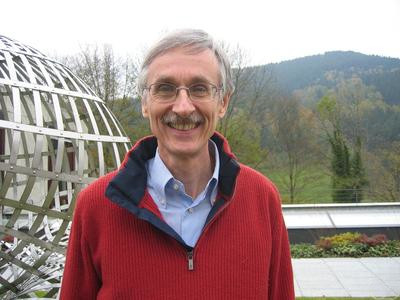
\includegraphics[height=0.34\textheight]{ch0_kunsch_2007.jpg}\\[1mm]
\imgcap{Hans Rudolf Künsch (2007)}
\imgcredit{https://commons.wikimedia.org/wiki/File:Hans-Rudolf_Künsch.jpg}{Foto: Renate Schmid (2007); CC BY-SA 2.0 de; Wikimedia Commons}
\end{column}
\end{columns}
\end{frame}

\begin{frame}{Bootstrap circular și bootstrap staționar}
\itemsize{\footnotesize}
\begin{itemize}
    \item \textbf{Bootstrap circular pe blocuri} (Politis și Romano, 1992; \refLahiri): așezăm datele pe un cerc, $x_{T+i} = x_i$
    \begin{itemize}
        \item Fiecare observație intră în $l$ blocuri: $E^*\bar x^* = \bar x$ exact (Seminarul 0, A5--A6)
    \end{itemize}
    \item \textbf{Bootstrap staționar} \refPR: lungimile blocurilor $\sim$ geometrice cu media $1/p$, începuturi uniforme, cu înfășurare
    \begin{itemize}
        \item Echivalent: la fiecare pas blocul continuă cu probabilitatea $1 - p$ sau sare într-un punct aleator cu probabilitatea $p$
        \item Seria reeșantionată este staționară; metoda este mai puțin sensibilă la alegerea lui $1/p$ decît MBB la alegerea lui $l$
    \end{itemize}
    \item Eficiență: MBB și CBB au eroarea pătratică medie asimptotică mai mică pentru varianță decît bootstrap staționar, la lungimile optime \refLahiri
    \item Bootstrap staționar este motorul testului Reality Check (White 2000) și al testului SPA (\atschlink{https://danpele.github.io/Advanced-Time-Series/RO/Cursuri/capitol1_evaluarea_prognozelor.pdf}{Capitolul 1})
\end{itemize}
\end{frame}

\begin{frame}{Alegerea lungimii blocului}
\itemsize{\footnotesize}
\begin{itemize}
    \item \refPW, corectată de \refPPW: estimări prin înlocuire ale lungimii medii optime a blocului
    \begin{itemize}
        \item $\hat b_{opt} = \Big(\dfrac{2\hat G^2}{\hat D}\Big)^{1/3} T^{1/3}$, $\quad \hat G = \sum_{|k|\le M}\lambda(k/M)\,|k|\,\hat\gamma_k$, $\quad \hat g = \sum_{|k|\le M}\lambda(k/M)\,\hat\gamma_k$
        \item $\hat D_{SB} = 2\hat g^2$, $\hat D_{CB} = \tfrac{4}{3}\hat g^2$; $\lambda$ nucleul flat-top (trapez); $M = 2\hat m$, $\hat m$ primul decalaj după care $K_T$ autocorelații sînt nesemnificative
    \end{itemize}
    \item Aceeași structură ca lățimea Andrews: termenul de deplasare $G$ raportat la termenul de varianță $D$, rata $T^{1/3}$
    \begin{itemize}
        \item Implementat în pachetul Python \texttt{arch} (\texttt{optimal\_block\_length}); codul nostru îl reproduce pînă la ultima zecimală
    \end{itemize}
    \item Datele noastre: aproximativ 145 de zile pentru pătratele randamentelor S\&P 500, 25 de luni pentru inflație, 0{,}8 pentru creșterea PIB (adică bootstrap i.i.d.)
\end{itemize}
\end{frame}

\begin{frame}{Wild bootstrap și limitele lui}
\itemsize{\footnotesize}
\begin{itemize}
    \item \textbf{Wild bootstrap} \refWu, \refLiu, \refMammen: $y_t^* = x_t'\hat\beta + \hat u_t\eta_t$, $\eta_t$ i.i.d., $E\eta_t = 0$, $E\eta_t^2 = 1$ (Rademacher sau distribuția în două puncte Mammen)
    \begin{itemize}
        \item Păstrează heteroscedasticitatea fiecărui $\hat u_t$; distruge orice autocorelație
        \item Valid cînd scorurile sînt o MDS: modele AR cu erori de tip GARCH \refGK
    \end{itemize}
    \item \textbf{Nu} este valid pentru prognoze suprapuse, proiecții locale sau media pătratelor randamentelor
    \begin{itemize}
        \item Dependent wild bootstrap \refShao: $\eta_t$ extrase dintr-un proces staționar cu corelația $a(|t-s|/l)$: wild ca formă, de tip bloc ca efect
    \end{itemize}
    \item Sieve bootstrap \refBuhlmann: estimăm un AR$(p)$ cu $p \to \infty$ și reeșantionăm reziduurile: eficient pentru procese liniare, fragil pentru cele neliniare
\end{itemize}
\end{frame}

\begin{frame}{Trei bootstrap-uri ale aceleiași medii}
\itemsize{\footnotesize}
\begin{center}
    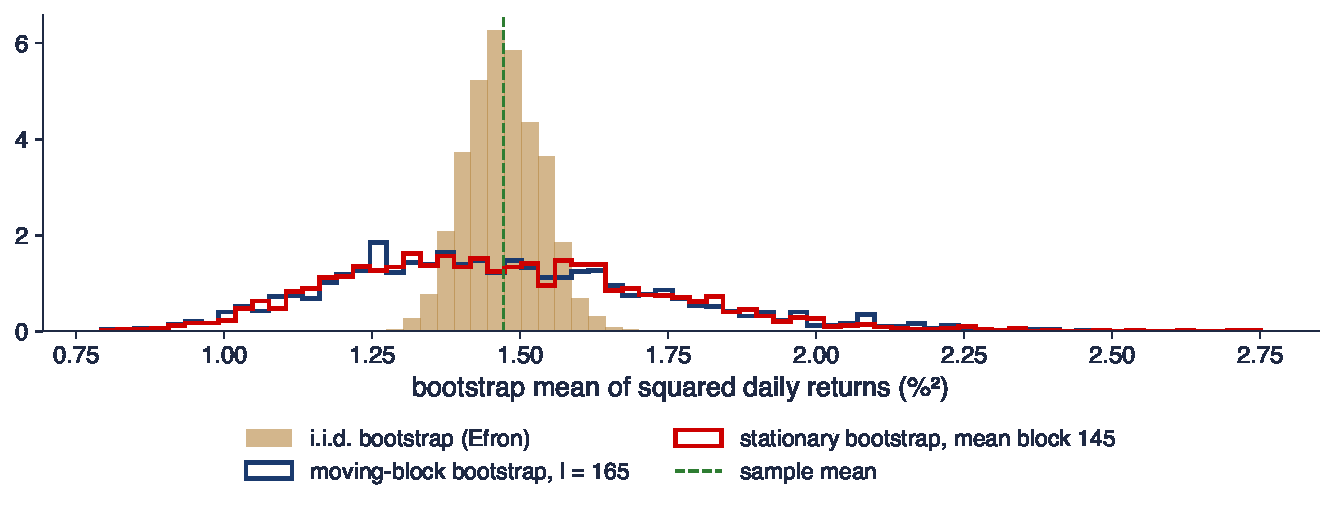
\includegraphics[width=0.97\textwidth,height=0.56\textheight,keepaspectratio]{ats_ch0_bootstrap.pdf}
\end{center}
\vspace{-0.25cm}
\begin{itemize}
    \item Media pătratelor randamentelor zilnice S\&P 500 ($1{,}472$, $T = 6\,714$); cîte 1999 de reeșantionări; lungimile blocurilor Politis--White
\end{itemize}
\quantlet{ATS\_ch0\_block\_bootstrap}{\qlurl{ATS_ch0_block_bootstrap}}
\end{frame}

\begin{frame}{Interpretarea celor trei bootstrap-uri}
\itemsize{\small}
\begin{itemize}
    \item Bootstrap i.i.d.: eroare standard $0{,}063$, egală cu cea naivă, $0{,}064$, cum spune teoria
    \begin{itemize}
        \item Bootstrap-urile pe blocuri: MBB $0{,}276$, CBB $0{,}268$, staționar $0{,}269$: de aproximativ 4{,}2 ori valoarea naivă
    \end{itemize}
    \item HAC cu lățimea Andrews: $0{,}152$ (de aproximativ 2{,}4 ori valoarea naivă): mai mică decît la bootstrap pe blocuri
    \begin{itemize}
        \item Lungimea blocului 145 față de lățimea Andrews de 17: două reguli prin înlocuire, două imagini diferite ale aceleiași ACF care scade lent
    \end{itemize}
    \item Cînd două metode valide diferă de două ori, le raportați pe amîndouă și explicați de ce: aici, volatilitatea volatilității are memorie lungă
\end{itemize}
\end{frame}

\begin{frame}{Eroarea standard bootstrap în funcție de lungimea blocului}
\itemsize{\footnotesize}
\begin{center}
    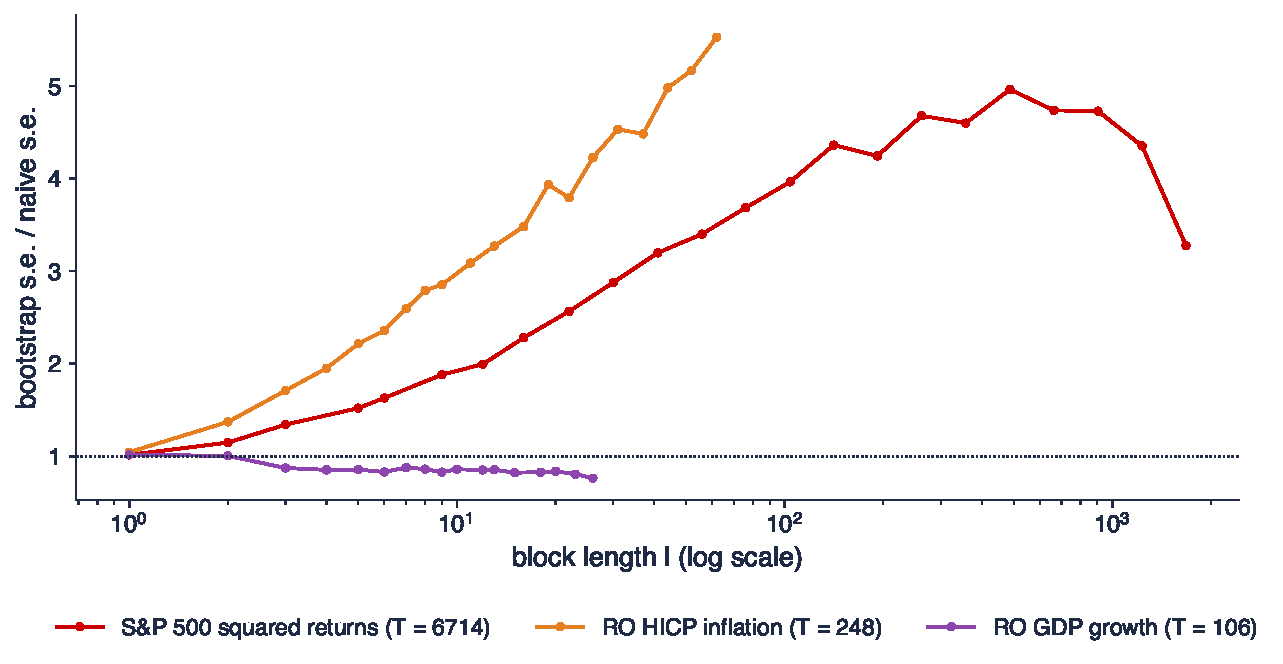
\includegraphics[width=0.97\textwidth,height=0.55\textheight,keepaspectratio]{ats_ch0_block_length.pdf}
\end{center}
\vspace{-0.25cm}
\begin{itemize}
    \item Bootstrap circular pe blocuri, 999 de reeșantionări pentru fiecare lungime; raportul față de eroarea standard naivă
\end{itemize}
\quantlet{ATS\_ch0\_block\_bootstrap}{\qlurl{ATS_ch0_block_bootstrap}}
\end{frame}

\begin{frame}{Interpretarea traiectoriilor în funcție de lungimea blocului}
\itemsize{\small}
\begin{itemize}
    \item $l = 1$ este bootstrap i.i.d.\ (raport 1); raportul crește odată cu $l$ cît timp $l$ este mai scurt decît memoria seriei
    \begin{itemize}
        \item Inflația: raportul 4{,}2 la lungimea Politis--White de 25 de luni
    \end{itemize}
    \item Creșterea PIB: aproape constant în jurul lui 1 (și puțin sub 1 pentru blocuri lungi): nu există dependență de captat
    \item Blocuri foarte lungi: puține blocuri distincte, varianță zgomotoasă și deplasată în jos (deplasarea lui $\hat\gamma_j$ la decalaje mari)
    \item Ce credeți? De ce curba inflației continuă să crească pînă cînd $l$ ajunge la aproximativ un sfert din eșantion?
\end{itemize}
\end{frame}

\begin{frame}{Mediile a șase serii: erori standard pe metode}
\itemsize{\footnotesize}
\begin{center}
\footnotesize
\begin{tabular}{lrrrrrrr}
\toprule
Seria & $T$ & Media & $\hat\rho_1$ & naivă & NW-A & boot.\ staț. & $t_{naive}$ / $t_{EWC}$ \\
\midrule
S\&P 500 de randamente & 6\,714 & 0{,}025 & \ensuremath{-}0{,}10 & 0{,}0148 & 0{,}0131 & 0{,}0129 & 1{,}67 / 2{,}07 \\
S\&P 500 pătrate & 6\,714 & 1{,}472 & 0{,}31 & 0{,}064 & 0{,}152 & 0{,}292 & 23{,}06 / 6{,}71 \\
randamente BET & 6\,670 & 0{,}064 & 0{,}11 & 0{,}0171 & 0{,}0188 & 0{,}0187 & 3{,}73 / 2{,}89 \\
EUR/RON & 5\,352 & 0{,}007 & 0{,}17 & 0{,}0038 & 0{,}0040 & 0{,}0039 & 1{,}86 / 1{,}73 \\
Creșterea PIB RO & 106 & 0{,}829 & \ensuremath{-}0{,}03 & 0{,}240 & 0{,}240 & 0{,}240 & 3{,}46 / 3{,}67 \\
Inflația RO & 248 & 4{,}799 & 0{,}98 & 0{,}218 & 1{,}131 & 0{,}957 & 22{,}05 / 5{,}92 \\
\bottomrule
\end{tabular}
\end{center}
\begin{itemize}
    \item NW-A: Newey--West cu lățimea Andrews; bootstrap staționar cu blocul mediu Politis--White; randamentele și variațiile în \% pe zi, PIB-ul în \% pe trimestru, inflația în \%
\end{itemize}
\end{frame}

\begin{frame}{Interpretarea tabelului}
\itemsize{\footnotesize}
\begin{itemize}
    \item S\&P 500: $t$ crește de la $1{,}67$ (naiv) la $2{,}03$ (fixed-$b$, valoarea critică $1{,}99$) și $2{,}07$ (EWC): randamentul mediu ($6{,}2\%$ pe an) devine semnificativ la limită
    \begin{itemize}
        \item Autocorelația negativă reduce eroarea standard: inferența robustă nu este întotdeauna mai conservatoare
    \end{itemize}
    \item EUR/RON: deprecierea medie a leului nu este semnificativă la 5\% prin nicio metodă ($t$ între $1{,}73$ și $1{,}86$)
    \item Inflația: $t$ scade de la $22{,}05$ la $5{,}92$ pentru $H_0: \mu = 0$; erorile standard cresc de aproximativ 4--5 ori
    \item Creșterea PIB: toate metodele sînt de acord; problema acolo sînt cele două trimestre de criză, nu dependența (Seminarul 0, B2)
\end{itemize}
\end{frame}

\begin{frame}{Recapitulare: bootstrap pentru date dependente}
\itemsize{\small}
\begin{itemize}
    \item Bootstrap i.i.d.\ reproduce eroarea standard naivă; reeșantionați în schimb blocuri
    \item MBB (Künsch 1989) este un estimator HAC Bartlett deghizat; CBB elimină deplasarea de capăt; bootstrap staționar păstrează staționaritatea
    \item Lungimea blocului $\propto T^{1/3}$, aleasă prin Politis--White; wild bootstrap tratează doar heteroscedasticitatea
\end{itemize}
\end{frame}


%=============================================================================
\section{Observații suprapuse: marja la termen și creșterea}
%=============================================================================

\begin{frame}{Studiu de caz: Estrella și Hardouvelis (1991)}
\itemsize{\small}
\begin{itemize}
    \item \refEH: prognozează panta curbei randamentelor creșterea reală din SUA? Regresia creșterii cumulate pe următoarele $k$ trimestre pe marja la termen
    \begin{itemize}
        \item $y_t^{(h)} = \dfrac{400}{h}\ln\dfrac{\mathrm{GDP}_{t+h}}{\mathrm{GDP}_t} = \beta_0 + \beta_1 (i^{10y}_t - i^{3m}_t) + u_t$, $\quad h = 4$
    \end{itemize}
    \item Suprapunere: $y_t^{(4)}$ și $y_{t+1}^{(4)}$ au trei trimestre comune, deci $u_t$ este cel puțin MA(3) sub $H_0$
    \begin{itemize}
        \item Soluția clasică: \refHH{} (nucleu trunchiat, $h - 1$ decalaje) sau Newey--West cu $L = h - 1$
    \end{itemize}
    \item Datele noastre: PIB real, randamentele titlurilor de stat la 10 ani și la 3 luni (medii trimestriale) din FRED, 1962Q1 -- 2025Q2, $T = 254$
    \item Același plan pentru proiecțiile locale (\atschlink{https://danpele.github.io/Advanced-Time-Series/RO/Cursuri/capitol3_modele_var_structurale_proiectii_locale.pdf}{Capitolul 3}) și pentru regresiile randamentelor pe orizonturi lungi (MFM)
\end{itemize}
\end{frame}

\begin{frame}{Marja la termen și creșterea viitoare}
\itemsize{\footnotesize}
\begin{center}
    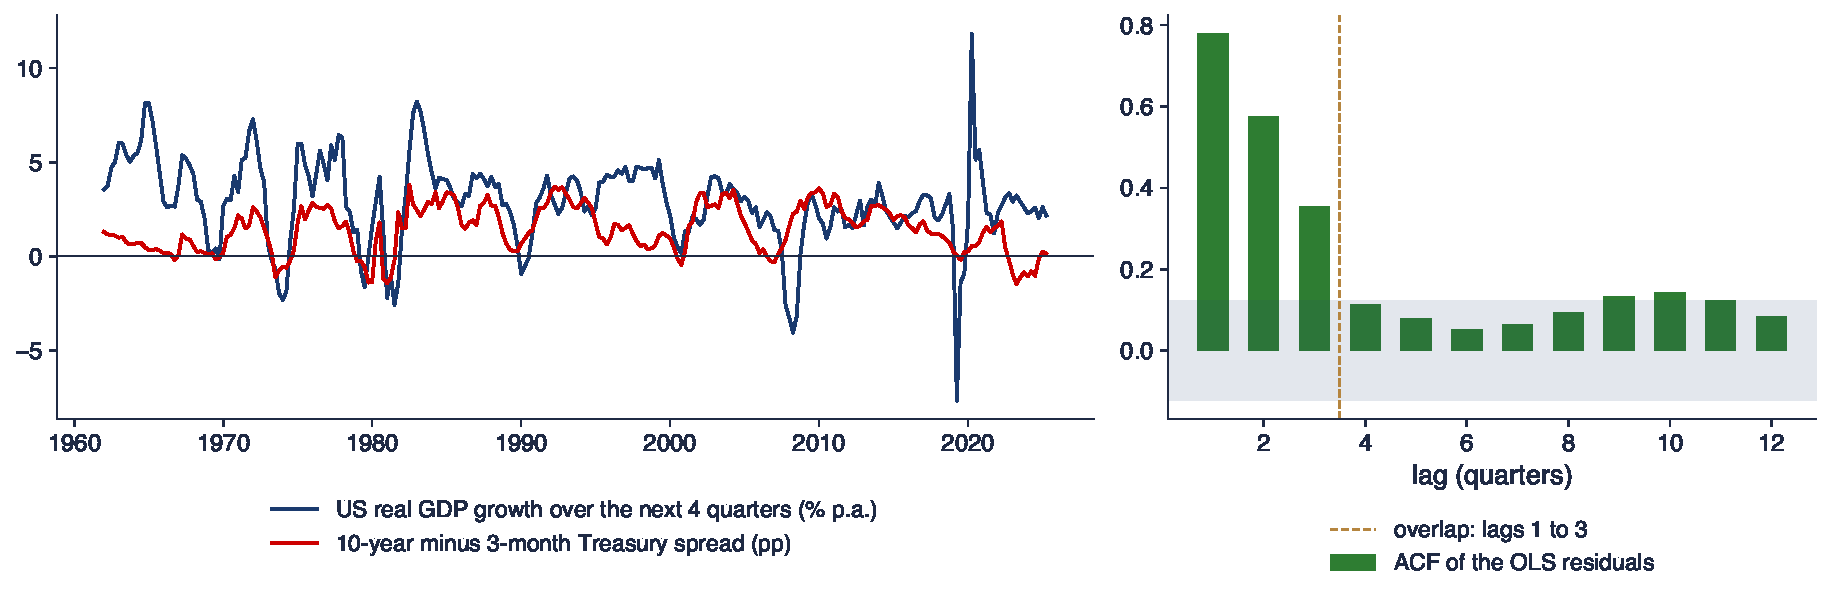
\includegraphics[width=0.97\textwidth,height=0.55\textheight,keepaspectratio]{ats_ch0_term_spread.pdf}
\end{center}
\vspace{-0.25cm}
\begin{itemize}
    \item Stînga: cele două serii; dreapta: ACF a reziduurilor MCMMP, $\hat\rho_1 = 0{,}78$, $\hat\rho_3 = 0{,}35$, $\hat\rho_4 = 0{,}11$
\end{itemize}
\quantlet{ATS\_ch0\_term\_spread}{\qlurl{ATS_ch0_term_spread}}
\end{frame}

\begin{frame}{O pantă, cinci erori standard}
\itemsize{\footnotesize}
\begin{center}
\footnotesize
\begin{tabular}{lrrr}
\toprule
Eroarea standard & $\widehat{se}(\hat\beta_1)$ & $t$ & Valoarea critică \\
\midrule
MCMMP clasic & 0{,}11 & 4{,}72 & 1.96 \\
White (doar heteroscedasticitate) & 0{,}10 & -- & 1.96 \\
Hansen--Hodrick, 3 decalaje & 0{,}20 & -- & 1.96 \\
Newey--West, 3 decalaje & 0{,}17 & 3{,}10 & 1.96 \\
NW, Andrews ($S = 14$) & 0{,}23 & 2{,}25 & 1.96 \\
NW, $S = 1{,}3\sqrt{T} = 21$, fixed-$b$ & 0{,}25 & 2{,}04 & 2{,}18 \\
\bottomrule
\end{tabular}
\end{center}
\begin{itemize}
    \item $\hat\beta_1 = 0{,}52$ pp de creștere anuală la fiecare pp de marjă, $R^2 = 0{,}08$
\end{itemize}
\end{frame}

\begin{frame}{Interpretarea regresiei marjei la termen}
\itemsize{\footnotesize}
\begin{itemize}
    \item Reziduurile sînt mai persistente decît MA(3) implicat de suprapunere ($\hat\rho_4 = 0{,}11$): 3 decalaje nu sînt suficiente
    \begin{itemize}
        \item Eroarea standard se dublează de la MCMMP clasic la fixed-$b$: $t$ scade de la $4{,}72$ la $2{,}04$, puțin sub valoarea critică $2{,}18$
    \end{itemize}
    \item Subeșantioane (NW, 3 decalaje): 1962--1988 $\hat\beta_1 = 1{,}12$ ($t = 4{,}6$); 1989--2025 $\hat\beta_1 = 0{,}15$ ($t = 0{,}9$)
    \begin{itemize}
        \item Puterea predictivă a marjei a scăzut după eșantionul original: o problemă de rupturi (\atschlink{https://danpele.github.io/Advanced-Time-Series/RO/Cursuri/capitol2_rupturi_structurale_modele_neliniare.pdf}{Capitolul 2}) și o problemă de evaluare în afara eșantionului (\atschlink{https://danpele.github.io/Advanced-Time-Series/RO/Cursuri/capitol1_evaluarea_prognozelor.pdf}{Capitolul 1})
    \end{itemize}
    \item Întîi inferența robustă, apoi stabilitatea: un $t$ de $4{,}72$ pe întregul eșantion ascunde ambele probleme
\end{itemize}
\end{frame}


%=============================================================================
\section{Testarea multiplă în cercetarea privind prognoza}
%=============================================================================

\begin{frame}{Data snooping}
\itemsize{\footnotesize}
\begin{itemize}
    \item \textbf{Data snooping}: refolosirea aceluiași set de date pentru a alege un model, o regulă sau o specificație, testat apoi pe aceleași date ca și cum ar fi fost ales dinainte
    \begin{itemize}
        \item \refLM: sortarea portofoliilor după caracteristici despre care se știe deja că sînt legate de randamente deplasează testele de evaluare a activelor
        \item \refHLZ: peste 300 de factori de randament publicați; un factor nou are nevoie de $t > 3$, nu de $t > 2$
    \end{itemize}
    \item Ratele de eroare pentru $K$ teste
    \begin{itemize}
        \item FWER: probabilitatea a cel puțin unei respingeri false; Bonferroni ($\alpha/K$) și Holm (pas cu pas descendent) o controlează
        \item FDR: proporția așteptată a respingerilor false printre respingeri, controlată de \refBH
    \end{itemize}
    \item În prognoză: multe modele, multe orizonturi, multe eșantioane; valoarea $p$ onestă este cea a \emph{căutării}, nu a cîștigătorului
\end{itemize}
\end{frame}

\begin{frame}{Cel mai bun dintre $K$ teste}
\itemsize{\footnotesize}
\begin{center}
    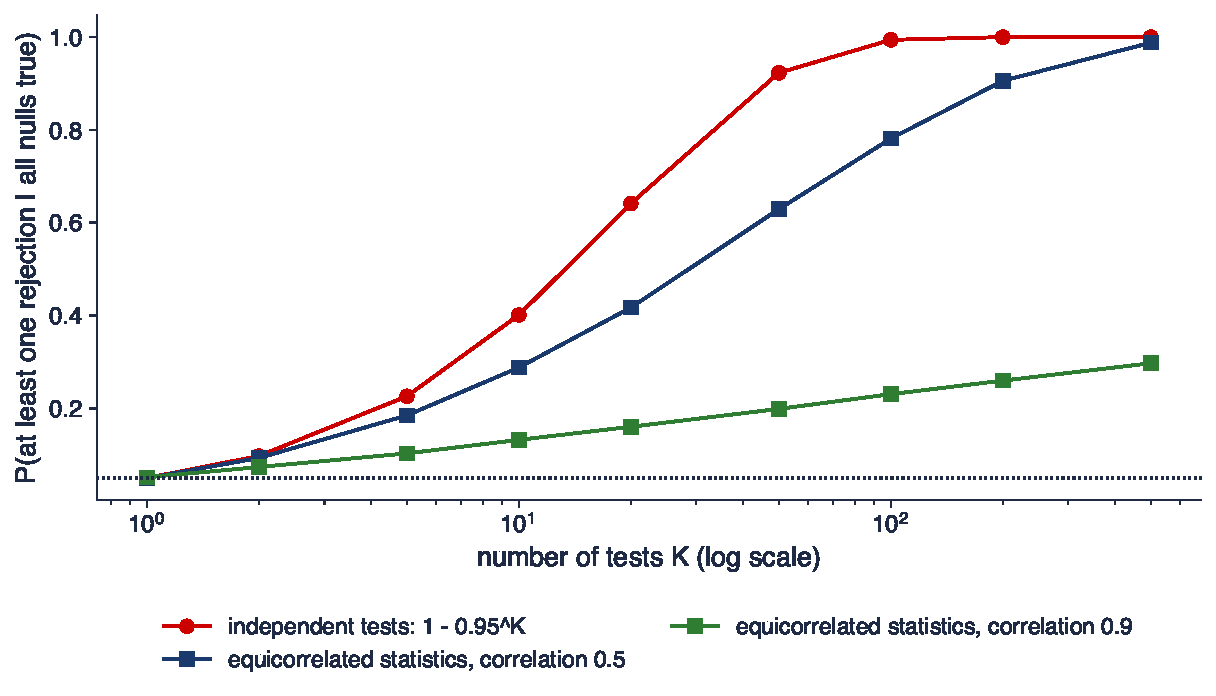
\includegraphics[width=0.97\textwidth,height=0.55\textheight,keepaspectratio]{ats_ch0_snooping.pdf}
\end{center}
\vspace{-0.25cm}
\begin{itemize}
    \item Probabilitatea ca cel mai mare $|t|$ din $K$ teste să depășească 1,96 cînd toate ipotezele nule sînt adevărate: statistici independente și echicorelate (20\,000 de simulări)
\end{itemize}
\quantlet{ATS\_ch0\_data\_snooping}{\qlurl{ATS_ch0_data_snooping}}
\end{frame}

\begin{frame}{Interpretarea erorii la nivelul familiei de teste}
\itemsize{\small}
\begin{itemize}
    \item Teste independente: FWER $64\%$ cu $K = 20$ și $99{,}4\%$ cu $K = 100$
    \begin{itemize}
        \item Bonferroni ar testa fiecare ipoteză la $0,05/20 = 0,0025$
    \end{itemize}
    \item Statistici corelate (reguli asemănătoare, eșantioane suprapuse): FWER $42\%$ ($K = 20$) și $78\%$ ($K = 100$) la corelația 0,5; $23\%$ la 0,9
    \begin{itemize}
        \item Bonferroni ignoră corelația și este conservator: bootstrap-ul maximului (slide-ul următor) o folosește
    \end{itemize}
    \item Ce credeți? Cu 50 de reguli de medie mobilă, cîte reguli „semnificative” vă așteptați să obțineți din întîmplare la 5\%?
\end{itemize}
\end{frame}

\begin{frame}{Studiu de caz: testul Reality Check, White (2000)}
\itemsize{\footnotesize}
\begin{itemize}
    \item $K$ modele comparate cu un reper; $f_{k,t}$ diferența de performanță (de exemplu randamentul regulii $k$ minus buy-and-hold) \refWhite
    \begin{itemize}
        \item $H_0: \max_k E f_{k,t} \le 0$ (niciun model nu bate reperul); $\quad \bar V = \max_k \sqrt{n}\,\bar f_k$
    \end{itemize}
    \item Distribuția sub $H_0$ prin bootstrap staționar al întregului vector $f_t$ (păstrează corelația dintre reguli și în timp):
    \begin{itemize}
        \item $\bar V^*_b = \max_k \sqrt{n}\,(\bar f^*_{k,b} - \bar f_k)$, $\quad p = B^{-1}\sum_b \mathbf{1}\{\bar V^*_b > \bar V\}$
    \end{itemize}
    \item \refSTW{} îl aplică pentru 7846 de reguli tehnice pe Dow Jones; \refHansen{} (SPA) și \refRW{} (StepM) îl rafinează: \atschlink{https://danpele.github.io/Advanced-Time-Series/RO/Cursuri/capitol1_evaluarea_prognozelor.pdf}{Capitolul 1}
    \item Aplicația noastră: 50 de reguli „poziție lungă dacă închiderea este peste media mobilă pe $n$ zile”, $n = 5, 10, \dots, 250$, pe BET, comparate cu buy-and-hold, fără costuri; bloc mediu de 10 zile
\end{itemize}
\end{frame}

\begin{frame}{Testul Reality Check pe BET}
\itemsize{\footnotesize}
\begin{center}
    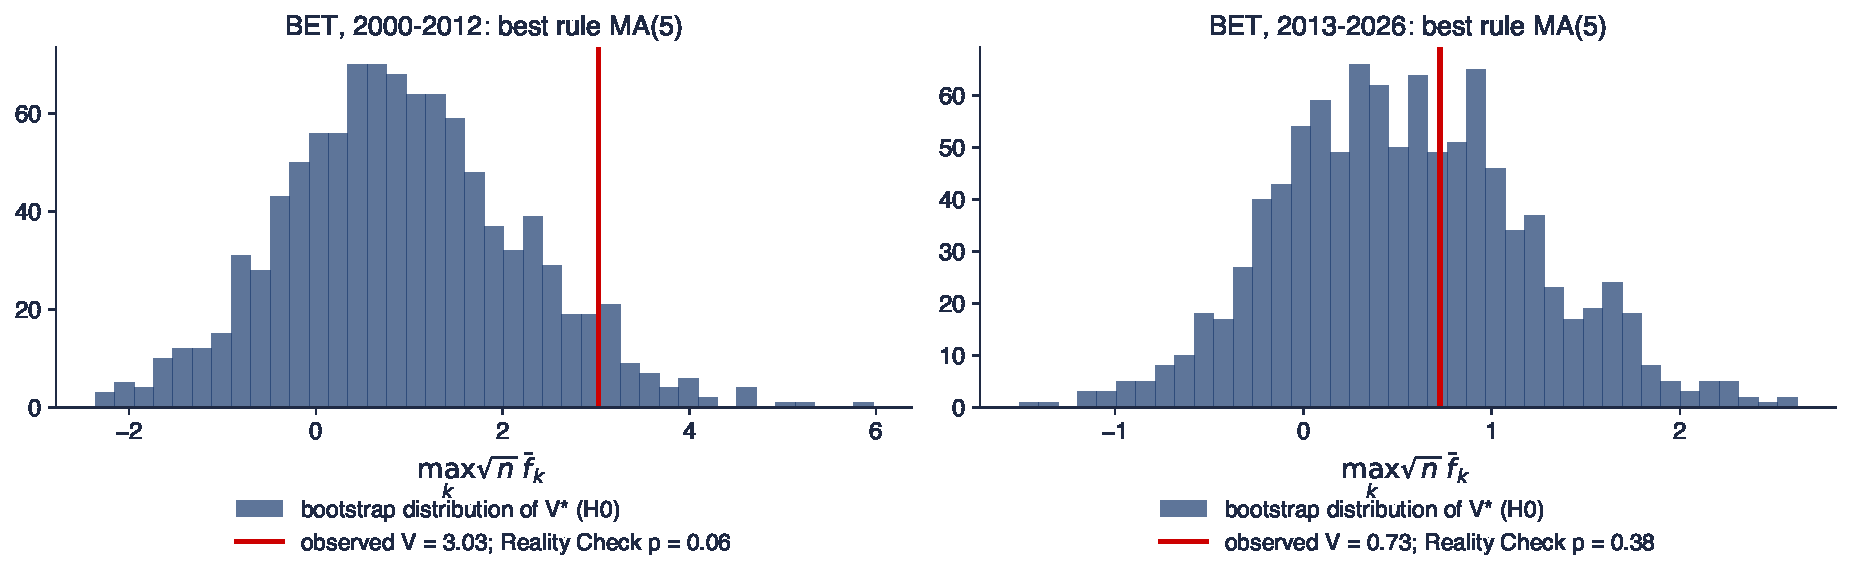
\includegraphics[width=0.97\textwidth,height=0.55\textheight,keepaspectratio]{ats_ch0_reality_check.pdf}
\end{center}
\vspace{-0.25cm}
\begin{itemize}
    \item Distribuția bootstrap a lui $\bar V^*$ sub $H_0$ (999 de reeșantionări prin bootstrap staționar) și valoarea observată $\bar V$; două subeșantioane
\end{itemize}
\quantlet{ATS\_ch0\_data\_snooping}{\qlurl{ATS_ch0_data_snooping}}
\end{frame}

\begin{frame}{Interpretarea testului Reality Check}
\itemsize{\footnotesize}
\begin{itemize}
    \item 2001--2012 ($n = 2\,993$ zile): cea mai bună regulă, MA(5), bate buy-and-hold cu $0{,}055\%$ pe zi, $t = 2{,}51$, $p$ naiv unilateral $= 0{,}006$
    \begin{itemize}
        \item Reality Check $p = 0{,}06$: nesemnificativ la 5\% după ce se ține seama de căutarea printre 50 de reguli
    \end{itemize}
    \item 2014--2026: aceeași regulă, $t = 0{,}97$, Reality Check $p = 0{,}38$: orice ar fi existat nu a supraviețuit
    \item Cîștigătoarea cu medie mobilă scurtă se potrivește cu $\hat\rho_1$ pozitiv al randamentelor BET (prețuri învechite), iar costurile de tranzacționare l-ar anula
    \item Preînregistrați universul de reguli și împărțirea eșantionului înainte de a vedea rezultatele (Etapa 1 a proiectului)
\end{itemize}
\end{frame}

\begin{frame}{Recapitulare: testarea multiplă}
\itemsize{\small}
\begin{itemize}
    \item Valoarea $p$ a celui mai bun dintre $K$ teste nu este valoarea $p$ a unui test specificat dinainte
    \item FWER (Bonferroni, Holm) sau FDR (Benjamini--Hochberg); pentru prognoze corelate: bootstrap pentru maxim (Reality Check)
    \item Testele de comparare a prognozelor (Diebold--Mariano, SPA, Model Confidence Set) sînt subiectul \atschlink{https://danpele.github.io/Advanced-Time-Series/RO/Cursuri/capitol1_evaluarea_prognozelor.pdf}{Capitolului 1}
\end{itemize}
\end{frame}


%=============================================================================
\section{Practica cercetării reproductibile}
%=============================================================================

\begin{frame}{Semințe și experimente Monte Carlo}
\itemsize{\small}
\begin{itemize}
    \item O singură sămînță pe proiect, fixată o dată: \texttt{rng = np.random.default\_rng(2026)}; transmiteți \texttt{rng} fiecărei funcții
    \begin{itemize}
        \item Rulări paralele: \texttt{np.random.SeedSequence(2026).spawn(k)} dă fluxuri independente; nu refolosiți niciodată o stare globală
    \end{itemize}
    \item Raportați ce face o simulare verificabilă
    \begin{itemize}
        \item DGP, $T$, numărul de replicări $R$, valorile inițiale eliminate, sămînța, eroarea standard Monte Carlo $\sqrt{p(1-p)/R}$
        \item Rezultatele nu trebuie să depindă de sămînță peste eroarea Monte Carlo: rulați din nou cu o a doua sămînță
    \end{itemize}
    \item Fiecare grafic și fiecare cifră din acest capitol sînt produse de un singur script cu sămînța 2026 (Quantlets/Ch\_00)
\end{itemize}
\end{frame}

\begin{frame}{Date versionate}
\itemsize{\small}
\begin{itemize}
    \item Datele macro sînt revizuite: PIB-ul descărcat azi nu este PIB-ul pe care l-a văzut un prognozator în timp real
    \begin{itemize}
        \item Vintage-uri în timp real: \refCS{} (Fed Philadelphia), ALFRED pentru seriile FRED; Eurostat revizuiește conturile naționale în fiecare trimestru
    \end{itemize}
    \item Salvați un instantaneu datat al fiecărei serii folosite, împreună cu interogarea care l-a produs
    \begin{itemize}
        \item Notați data descărcării, codul setului de date (de exemplu \texttt{namq\_10\_gdp}) și o sumă de control (\texttt{sha256}) a fișierului
        \item Datele de piață ale cursului sînt salvate o singură dată și se termină pe 18 septembrie 2026: fiecare student obține aceleași cifre
    \end{itemize}
    \item O prognoză evaluată pe date revizuite răspunde la altă întrebare decît cea pusă în timp real
\end{itemize}
\end{frame}

\begin{frame}{Pachete de replicare}
\itemsize{\small}
\begin{itemize}
    \item Ce cer acum revistele de economie \refVilhuber, \refCM
    \begin{itemize}
        \item un README cu declarația de disponibilitate a datelor, ordinea scripturilor și timpul de rulare estimat
        \item cod care regenerează fiecare tabel și grafic din datele brute, fără pași manuali
        \item mediul de calcul: \texttt{requirements.txt} cu versiuni sau un notebook Colab
    \end{itemize}
    \item Pentru proiectul ATS (Etapa 2)
    \begin{itemize}
        \item un repository GitHub: \texttt{data/}, \texttt{code/}, \texttt{output/}, README, AI\_USE.md, AI\_ERRORS.md
        \item o singură comandă sau un singur notebook reproduce fiecare rezultat din raport
    \end{itemize}
    \item Testul: un coleg clonează repository-ul pe un calculator curat și obține aceleași cifre
\end{itemize}
\end{frame}

\begin{frame}{Preînregistrarea și planul de analiză}
\itemsize{\small}
\begin{itemize}
    \item Etapa 1 a proiectului fixează, înaintea oricărei estimări:
    \begin{itemize}
        \item ipoteza, eșantionul și împărțirea lui (estimare, evaluare), reperul
        \item metoda de inferență (regula HAC, bootstrap, valorile critice) și corecția pentru testarea multiplă
        \item lista specificațiilor care vor fi raportate, toate
    \end{itemize}
    \item Motivul: multitudinea de alegeri mici transformă analiza într-o căutare implicită
    \begin{itemize}
        \item Orice abatere de la plan este permisă, dar raportată, cu motivul ei
    \end{itemize}
    \item Un asistent AI face căutarea mai ieftină: AI\_USE.md consemnează prompturile care au influențat o decizie
\end{itemize}
\end{frame}

\begin{frame}{Recapitulare: cercetarea reproductibilă}
\itemsize{\small}
\begin{itemize}
    \item Fixați sămînța o dată, transmiteți generatorul, raportați $R$ și eroarea Monte Carlo
    \item Instantanee de date datate, cu sumă de control; vintage-uri în timp real cînd întrebarea privește prognoza în timp real
    \item Un pachet de replicare care rulează de la datele brute pînă la fiecare cifră; un plan fixat înaintea rezultatelor
\end{itemize}
\end{frame}


%=============================================================================
\section{AI în descoperirea științifică}
%=============================================================================

\begin{frame}{O întrebare deschisă: inferență validă pentru media unei serii aproape integrate}
\itemsize{\small}
\begin{itemize}
    \item A fost inflația din România, în medie, la nivelul țintei BNR din 2013? Formal, $H_0: \mu = 2,5$ pentru rata anuală IAPC, 164 de luni pînă în august 2026
    \begin{itemize}
        \item $\hat\rho_1 = 0{,}99$: seria este aproape de o rădăcină unitară și suprapusă prin construcție
    \end{itemize}
    \item Deschis: nicio regulă cu nucleu, EWC sau bootstrap nu controlează mărimea la această persistență (studiul Monte Carlo de mai sus)
    \begin{itemize}
        \item \refMuller{} și \refLLS{} descriu frontiera; ce test ar trebui să folosească un analist al băncii centrale cu 10--15 ani de date?
    \end{itemize}
    \item O întrebare cu conținut de politică economică (credibilitatea țintei) și un nucleu metodologic (inferență HAR la $\phi \approx 1$)
\end{itemize}
\end{frame}

\begin{frame}{Bucla de descoperire asistată de AI}
\itemsize{\footnotesize}
\begin{itemize}
    \item \textbf{Literatura}: \aiprompt{"Listează testele publicate pentru media unei serii foarte persistente, din 2010 încoace, cu DOI și planul Monte Carlo."}
    \begin{itemize}
        \item Verificare: rezolvați fiecare DOI în Crossref; citiți voi tabelele de mărime (Semantic Scholar, Elicit pentru căutare)
    \end{itemize}
    \item \textbf{Ipoteză și cod}: \aiprompt{"Scrie cod Python pentru testele NW fixed-b și EWC ale unei medii și un Monte Carlo al mărimii lor la phi = 0,98, T = 164."}
    \begin{itemize}
        \item Verificare: reproduceți întîi o mărime publicată (de exemplu tabelele LLSW), apoi modificați un singur element pe rînd
    \end{itemize}
    \item \textbf{Robustețe și critică}: \aiprompt{"Joacă rolul unui recenzent ostil: de ce ar putea acest test al mediei inflației să inducă în eroare?"}
    \begin{itemize}
        \item De așteptat: rupturi în medie (2013, 2022), diferența IPC--IAPC, suprapunerea, alegerea datei de început
    \end{itemize}
    \item \textbf{Verificările făcute de om}: formulele, momentul în care informația devine disponibilă (fără look-ahead), fiecare cifră pe cod; instrumentele sînt generice (Claude, ChatGPT, Gemini, Copilot)
\end{itemize}
\end{frame}

\begin{frame}{Mini-studiu de caz: o ipoteză, șase răspunsuri}
\itemsize{\footnotesize}
\begin{center}
    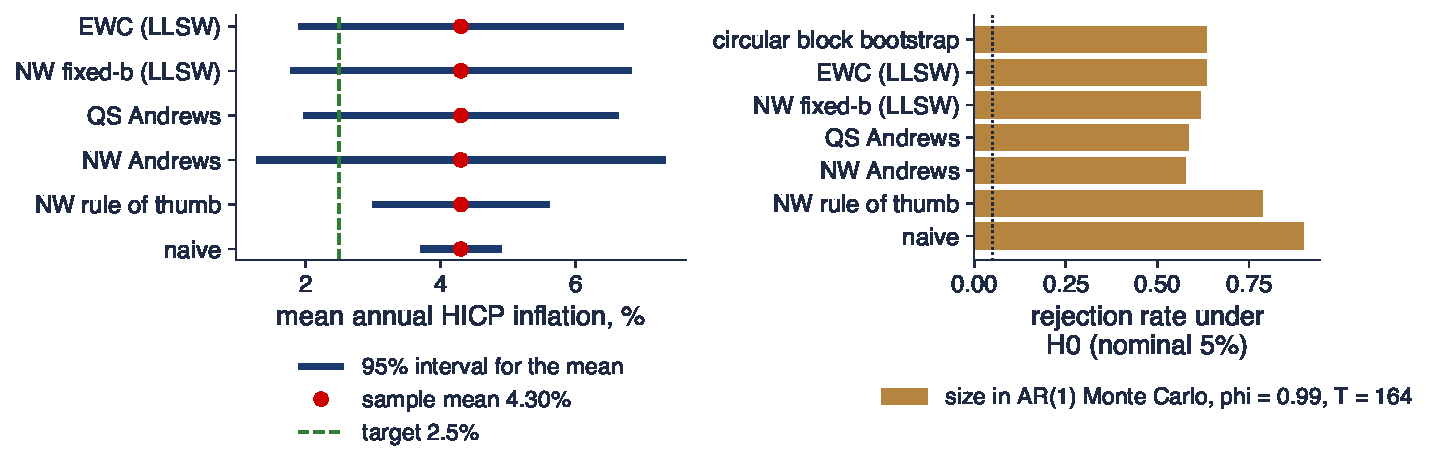
\includegraphics[width=0.97\textwidth,height=0.52\textheight,keepaspectratio]{ats_ch0_ai_minicase.pdf}
\end{center}
\vspace{-0.25cm}
\begin{itemize}
    \item Stînga: intervale de 95\% pentru media inflației IAPC din 2013 (media $4{,}30\%$); dreapta: mărimea fiecărui test într-un Monte Carlo cu AR(1) estimat, $\phi = 0{,}99$, $T = 164$
\end{itemize}
\quantlet{ATS\_ch0\_ai\_discovery}{\qlurl{ATS_ch0_ai_discovery}}
\end{frame}

\begin{frame}{Interpretarea mini-studiului de caz}
\itemsize{\footnotesize}
\begin{itemize}
    \item O propunere tipică a unui asistent: „NW cu $\lfloor 4(T/100)^{2/9}\rfloor$ decalaje” dă $t = 2{,}69$ și respinge $\mu = 2,5$
    \begin{itemize}
        \item Mărimea lui efectivă la această persistență: $79\%$ în loc de 5\%; testul naiv: $90\%$
    \end{itemize}
    \item NW-Andrews ($t = 1{,}17$), fixed-$b$ ($t = 1{,}59$, valoarea critică $2{,}23$) și EWC ($t = 1{,}63$, $\nu = 12$) nu resping
    \begin{itemize}
        \item Dar mărimile lor sînt tot $58\%$--$63\%$: nici nerespingerea nu este o dovadă în favoarea țintei
    \end{itemize}
    \item Concluzia onestă: cu 14 ani dintr-o serie aproape integrată, datele nu pot tranșa întrebarea; aceasta este partea deschisă
\end{itemize}
\end{frame}

\begin{frame}{Idee de proiect}
\itemsize{\footnotesize}
\begin{itemize}
    \item \textbf{Întrebarea}: ce test HAR este fiabil pentru media inflației din România și din zona euro, 2005--2026?
    \begin{itemize}
        \item Replicați întîi: un tabel de mărime din \refLLSW{} (planul lor AR(1)); explicați orice diferență
    \end{itemize}
    \item \textbf{Extensia}
    \begin{itemize}
        \item adăugați testele din \refMuller; calibrați studiul Monte Carlo pe datele IAPC ale tuturor țărilor UE (Eurostat)
        \item raportați mărimea și puterea pe o frontieră pentru fiecare țară; testați ipoteza țintei cu testul care controlează mărimea
    \end{itemize}
    \item \textbf{Livrabile}: un plan de analiză datat; un pachet de replicare; AI\_USE.md cu prompturile care au influențat decizii; AI\_ERRORS.md cu fiecare referință inventată sau cifră greșită depistată
\end{itemize}
\end{frame}


%=============================================================================
\section{Concluzii}
%=============================================================================

\begin{frame}{Idei de reținut}
\itemsize{\small}
\begin{itemize}
    \item Precizia unei medii sau a unei pante este dată de varianța de termen lung $\Omega = 2\pi f(0)$, nu de $\gamma_0$
    \item Ergodicitatea dă consistența; structura MDS sau mixing dă TLC; estimatorul HAC dă eroarea standard
    \item Nucleul, lățimea de bandă și valorile critice sînt o singură decizie: implicit, NW cu $1{,}3\sqrt{T}$ și fixed-$b$ sau EWC
    \item Bootstrap pe blocuri reeșantionează dependența; wild bootstrap nu o face
    \item Rădăcinile aproape unitare le înving pe toate: măsurați mărimea testului prin Monte Carlo, la persistența datelor voastre
    \item Căutările au nevoie de valori $p$ ajustate pentru căutare; proiectele au nevoie de pachete de replicare și de un plan fixat dinainte
\end{itemize}
\end{frame}

\begin{frame}{Autoevaluare}
\itemsize{\small}
\begin{itemize}
    \item Care este varianța de termen lung a unui MA(1) cu $\theta = -0,5$ și $\sigma^2 = 1$?
    \item De ce poate nucleul trunchiat să dea o varianță negativă, iar nucleul Bartlett nu?
    \item Ce eroare standard ați folosi pentru media randamentelor zilnice S\&P 500?
    \item Ce eroare standard ați folosi pentru media pătratelor lor?
    \item De ce este wild bootstrap invalid pentru o regresie cu creșteri pe patru trimestre suprapuse?
    \item Ați încercat 40 de specificații și o raportați pe cea mai bună: ce valoare $p$ ar trebui să raportați?
\end{itemize}
\end{frame}

\begin{frame}{Capitolul următor și lecturi suplimentare}
\itemsize{\small}
\begin{itemize}
    \item \textbf{Urmează}: \atschlink{https://danpele.github.io/Advanced-Time-Series/RO/Cursuri/capitol1_evaluarea_prognozelor.pdf}{Capitolul 1}, evaluarea prognozelor, reguli de scor și combinarea prognozelor
    \begin{itemize}
        \item Diebold--Mariano este un test $t$ HAC pe diferențele de pierdere; SPA și Model Confidence Set folosesc bootstrap staționar din acest capitol
    \end{itemize}
    \item \textbf{Lecturi suplimentare}
    \begin{itemize}
        \item Teorie: \refHamilton{} (cap.\ 7 și 10), \refBradley, \refLahiri
        \item Practică: \refLLSW, \refLLS, \refMuller
        \item Data snooping: \refWhite, \refHansen, \refRW, \refHLZ
    \end{itemize}
    \item \textbf{Cod}
    \begin{itemize}
        \item Quantlets: \href{https://github.com/danpele/Advanced-Time-Series/tree/main/Quantlets/Ch_00}{github.com/danpele/Advanced-Time-Series/tree/main/Quantlets/Ch\_00}
        \item Python: \texttt{statsmodels} (\texttt{cov\_type="HAC"}), \texttt{arch.bootstrap} (\texttt{StationaryBootstrap}, \texttt{optimal\_block\_length}, \texttt{SPA})
    \end{itemize}
\end{itemize}
\end{frame}


%=============================================================================
\section{Bibliografie}
%=============================================================================

\begin{frame}{Bibliografie (1/4)}
\itemsize{\tiny}
\begin{itemize}
    \item Andrews, D.W.K. (1991). \href{https://doi.org/10.2307/2938229}{Heteroskedasticity and autocorrelation consistent covariance matrix estimation}. \emph{Econometrica}, 59(3), 817--858.
    \item Andrews, D.W.K., Monahan, J.C. (1992). \href{https://doi.org/10.2307/2951574}{An improved heteroskedasticity and autocorrelation consistent covariance matrix estimator}. \emph{Econometrica}, 60(4), 953--966.
    \item Angelopoulos, A.N., Bates, S. (2023). \href{https://doi.org/10.1561/2200000101}{Conformal prediction: a gentle introduction}. \emph{Foundations and Trends in Machine Learning}, 16(4), 494--591.
    \item Baltagi, B.H. (2021). \href{https://doi.org/10.1007/978-3-030-53953-5}{\emph{Econometric Analysis of Panel Data}} (6th ed.). Springer.
    \item Benjamini, Y., Hochberg, Y. (1995). \href{https://doi.org/10.1111/j.2517-6161.1995.tb02031.x}{Controlling the false discovery rate: a practical and powerful approach to multiple testing}. \emph{Journal of the Royal Statistical Society B}, 57(1), 289--300.
    \item Billingsley, P. (1961). \href{https://doi.org/10.1090/S0002-9939-1961-0126871-X}{The Lindeberg--Lévy theorem for martingales}. \emph{Proceedings of the American Mathematical Society}, 12(5), 788--792.
    \item Birkhoff, G.D. (1931). \href{https://doi.org/10.1073/pnas.17.2.656}{Proof of the ergodic theorem}. \emph{Proceedings of the National Academy of Sciences}, 17(12), 656--660.
    \item Bradley, R.C. (2005). \href{https://doi.org/10.1214/154957805100000104}{Basic properties of strong mixing conditions. A survey and some open questions}. \emph{Probability Surveys}, 2, 107--144.
    \item Brown, B.M. (1971). \href{https://doi.org/10.1214/aoms/1177693494}{Martingale central limit theorems}. \emph{The Annals of Mathematical Statistics}, 42(1), 59--66.
    \item Bühlmann, P. (1997). \href{https://doi.org/10.2307/3318584}{Sieve bootstrap for time series}. \emph{Bernoulli}, 3(2), 123--148.
    \item Carrasco, M., Chen, X. (2002). \href{https://doi.org/10.1017/S0266466602181023}{Mixing and moment properties of various GARCH and stochastic volatility models}. \emph{Econometric Theory}, 18(1), 17--39.
    \item Christensen, G., Miguel, E. (2018). \href{https://doi.org/10.1257/jel.20171350}{Transparency, reproducibility, and the credibility of economics research}. \emph{Journal of Economic Literature}, 56(3), 920--980.
    \item Croushore, D., Stark, T. (2001). \href{https://doi.org/10.1016/S0304-4076(01)00072-0}{A real-time data set for macroeconomists}. \emph{Journal of Econometrics}, 105(1), 111--130.
    \item Durbin, J., Koopman, S.J. (2012). \href{https://doi.org/10.1093/acprof:oso/9780199641178.001.0001}{\emph{Time Series Analysis by State Space Methods}} (2nd ed.). Oxford University Press.
    \item Efron, B. (1979). \href{https://doi.org/10.1214/aos/1176344552}{Bootstrap methods: another look at the jackknife}. \emph{The Annals of Statistics}, 7(1), 1--26.
\end{itemize}
\end{frame}

\begin{frame}{Bibliografie (2/4)}
\itemsize{\tiny}
\begin{itemize}
    \item Estrella, A., Hardouvelis, G.A. (1991). \href{https://doi.org/10.1111/j.1540-6261.1991.tb02674.x}{The term structure as a predictor of real economic activity}. \emph{The Journal of Finance}, 46(2), 555--576.
    \item Gonçalves, S., Kilian, L. (2004). \href{https://doi.org/10.1016/j.jeconom.2003.10.030}{Bootstrapping autoregressions with conditional heteroskedasticity of unknown form}. \emph{Journal of Econometrics}, 123(1), 89--120.
    \item Granger, C.W.J., Newbold, P. (1974). \href{https://doi.org/10.1016/0304-4076(74)90034-7}{Spurious regressions in econometrics}. \emph{Journal of Econometrics}, 2(2), 111--120.
    \item Hamilton, J.D. (1994). \href{https://doi.org/10.2307/j.ctv14jx6sm}{\emph{Time Series Analysis}}. Princeton University Press.
    \item Hansen, L.P., Hodrick, R.J. (1980). \href{https://doi.org/10.1086/260910}{Forward exchange rates as optimal predictors of future spot rates: an econometric analysis}. \emph{Journal of Political Economy}, 88(5), 829--853.
    \item Hansen, P.R. (2005). \href{https://doi.org/10.1198/073500105000000063}{A test for superior predictive ability}. \emph{Journal of Business \& Economic Statistics}, 23(4), 365--380.
    \item Harvey, C.R., Liu, Y., Zhu, H. (2016). \href{https://doi.org/10.1093/rfs/hhv059}{\ldots and the cross-section of expected returns}. \emph{The Review of Financial Studies}, 29(1), 5--68.
    \item Huang, C., Petukhina, A. (2022). \href{https://doi.org/10.1007/978-3-031-13584-2}{\emph{Applied Time Series Analysis and Forecasting with Python}}. Springer.
    \item Hyndman, R.J., Athanasopoulos, G. (2021). \href{https://otexts.com/fpp3/}{\emph{Forecasting: Principles and Practice}} (3rd ed.). OTexts.
    \item Ibragimov, I.A. (1962). \href{https://doi.org/10.1137/1107036}{Some limit theorems for stationary processes}. \emph{Theory of Probability and Its Applications}, 7(4), 349--382.
    \item Kiefer, N.M., Vogelsang, T.J. (2002). \href{https://doi.org/10.1111/1468-0262.00366}{Heteroskedasticity-autocorrelation robust standard errors using the Bartlett kernel without truncation}. \emph{Econometrica}, 70(5), 2093--2095.
    \item Kiefer, N.M., Vogelsang, T.J. (2005). \href{https://doi.org/10.1017/S0266466605050565}{A new asymptotic theory for heteroskedasticity-autocorrelation robust tests}. \emph{Econometric Theory}, 21(6), 1130--1164.
    \item Kiefer, N.M., Vogelsang, T.J., Bunzel, H. (2000). \href{https://doi.org/10.1111/1468-0262.00128}{Simple robust testing of regression hypotheses}. \emph{Econometrica}, 68(3), 695--714.
    \item Kilian, L., Lütkepohl, H. (2017). \href{https://doi.org/10.1017/9781108164818}{\emph{Structural Vector Autoregressive Analysis}}. Cambridge University Press.
    \item Künsch, H.R. (1989). \href{https://doi.org/10.1214/aos/1176347265}{The jackknife and the bootstrap for general stationary observations}. \emph{The Annals of Statistics}, 17(3), 1217--1241.
\end{itemize}
\end{frame}

\begin{frame}{Bibliografie (3/4)}
\itemsize{\tiny}
\begin{itemize}
    \item Lahiri, S.N. (2003). \href{https://doi.org/10.1007/978-1-4757-3803-2}{\emph{Resampling Methods for Dependent Data}}. Springer.
    \item Lazarus, E., Lewis, D.J., Stock, J.H. (2021). \href{https://doi.org/10.3982/ECTA15404}{The size-power tradeoff in HAR inference}. \emph{Econometrica}, 89(5), 2497--2516.
    \item Lazarus, E., Lewis, D.J., Stock, J.H., Watson, M.W. (2018). \href{https://doi.org/10.1080/07350015.2018.1506926}{HAR inference: recommendations for practice}. \emph{Journal of Business \& Economic Statistics}, 36(4), 541--559.
    \item Liu, R.Y. (1988). \href{https://doi.org/10.1214/aos/1176351062}{Bootstrap procedures under some non-i.i.d.\ models}. \emph{The Annals of Statistics}, 16(4), 1696--1708.
    \item Lo, A.W., MacKinlay, A.C. (1990). \href{https://doi.org/10.1093/rfs/3.3.431}{Data-snooping biases in tests of financial asset pricing models}. \emph{The Review of Financial Studies}, 3(3), 431--467.
    \item Lütkepohl, H. (2005). \href{https://doi.org/10.1007/978-3-540-27752-1}{\emph{New Introduction to Multiple Time Series Analysis}}. Springer.
    \item Mammen, E. (1993). \href{https://doi.org/10.1214/aos/1176349025}{Bootstrap and wild bootstrap for high dimensional linear models}. \emph{The Annals of Statistics}, 21(1), 255--285.
    \item Mokkadem, A. (1988). \href{https://doi.org/10.1016/0304-4149(88)90045-2}{Mixing properties of ARMA processes}. \emph{Stochastic Processes and their Applications}, 29(2), 309--315.
    \item Müller, U.K. (2014). \href{https://doi.org/10.1080/07350015.2014.931238}{HAC corrections for strongly autocorrelated time series}. \emph{Journal of Business \& Economic Statistics}, 32(3), 311--322.
    \item Newey, W.K., West, K.D. (1987). \href{https://doi.org/10.2307/1913610}{A simple, positive semi-definite, heteroskedasticity and autocorrelation consistent covariance matrix}. \emph{Econometrica}, 55(3), 703--708.
    \item Newey, W.K., West, K.D. (1994). \href{https://doi.org/10.2307/2297912}{Automatic lag selection in covariance matrix estimation}. \emph{The Review of Economic Studies}, 61(4), 631--653.
    \item Patton, A., Politis, D.N., White, H. (2009). \href{https://doi.org/10.1080/07474930802459016}{Correction to ``Automatic block-length selection for the dependent bootstrap''}. \emph{Econometric Reviews}, 28(4), 372--375.
    \item Petropoulos, F., Apiletti, D., Assimakopoulos, V., Babai, M.Z., et al.\ (2022). \href{https://doi.org/10.1016/j.ijforecast.2021.11.001}{Forecasting: theory and practice}. \emph{International Journal of Forecasting}, 38(3), 705--871.
    \item Phillips, P.C.B. (1986). \href{https://doi.org/10.1016/0304-4076(86)90001-1}{Understanding spurious regressions in econometrics}. \emph{Journal of Econometrics}, 33(3), 311--340.
    \item Phillips, P.C.B., Solo, V. (1992). \href{https://doi.org/10.1214/aos/1176348666}{Asymptotics for linear processes}. \emph{The Annals of Statistics}, 20(2), 971--1001.
\end{itemize}
\end{frame}

\begin{frame}{Bibliografie (4/4)}
\itemsize{\tiny}
\begin{itemize}
    \item Politis, D.N., Romano, J.P. (1994). \href{https://doi.org/10.1080/01621459.1994.10476870}{The stationary bootstrap}. \emph{Journal of the American Statistical Association}, 89(428), 1303--1313.
    \item Politis, D.N., White, H. (2004). \href{https://doi.org/10.1081/ETC-120028836}{Automatic block-length selection for the dependent bootstrap}. \emph{Econometric Reviews}, 23(1), 53--70.
    \item Romano, J.P., Wolf, M. (2005). \href{https://doi.org/10.1111/j.1468-0262.2005.00615.x}{Stepwise multiple testing as formalized data snooping}. \emph{Econometrica}, 73(4), 1237--1282.
    \item Rosenblatt, M. (1956). \href{https://doi.org/10.1073/pnas.42.1.43}{A central limit theorem and a strong mixing condition}. \emph{Proceedings of the National Academy of Sciences}, 42(1), 43--47.
    \item Shao, X. (2010). \href{https://doi.org/10.1198/jasa.2009.tm08744}{The dependent wild bootstrap}. \emph{Journal of the American Statistical Association}, 105(489), 218--235.
    \item Shumway, R.H., Stoffer, D.S. (2017). \href{https://doi.org/10.1007/978-3-319-52452-8}{\emph{Time Series Analysis and Its Applications}} (4th ed.). Springer.
    \item Singh, K. (1981). \href{https://doi.org/10.1214/aos/1176345636}{On the asymptotic accuracy of Efron's bootstrap}. \emph{The Annals of Statistics}, 9(6), 1187--1195.
    \item Sullivan, R., Timmermann, A., White, H. (1999). \href{https://doi.org/10.1111/0022-1082.00163}{Data-snooping, technical trading rule performance, and the bootstrap}. \emph{The Journal of Finance}, 54(5), 1647--1691.
    \item Sun, Y., Phillips, P.C.B., Jin, S. (2008). \href{https://doi.org/10.1111/j.0012-9682.2008.00822.x}{Optimal bandwidth selection in heteroskedasticity--autocorrelation robust testing}. \emph{Econometrica}, 76(1), 175--194.
    \item Vilhuber, L. (2020). \href{https://doi.org/10.1162/99608f92.4f6b9e67}{Reproducibility and replicability in economics}. \emph{Harvard Data Science Review}, 2(4).
    \item White, H. (1980). \href{https://doi.org/10.2307/1912934}{A heteroskedasticity-consistent covariance matrix estimator and a direct test for heteroskedasticity}. \emph{Econometrica}, 48(4), 817--838.
    \item White, H. (2000). \href{https://doi.org/10.1111/1468-0262.00152}{A reality check for data snooping}. \emph{Econometrica}, 68(5), 1097--1126.
    \item Wu, C.F.J. (1986). \href{https://doi.org/10.1214/aos/1176350142}{Jackknife, bootstrap and other resampling methods in regression analysis}. \emph{The Annals of Statistics}, 14(4), 1261--1295.
\end{itemize}
\end{frame}

\end{document}
